\chapter{Análisis y Resultados}

En este capítulo se describe el proceso de selección de variables a considerar en el estudio,  con las cuales se ejecutará el algoritmo X-Means. Luego se presentan los resultados obtenidos y sus respectivos análisis.

\section{Variables}
Las variables seleccionadas tanto para establecimientos como para las matrículas, que se encuentran individualizadas en los anexos \ref{tab:atributos_establecimientos} y \ref{tab:atributos_matriculas} respectivamente, fueron filtradas según los porcentajes que ocupan cada uno de sus valores. Es decir, se contabilizó la cantidad de repeticiones para un valor dentro de la variable y se calculó su porcentaje. Con esto de clasificaron en 3 categorías según su importancia:


\begin{itemize}
    \item Baja: cuando el porcentaje de aparición de un valor es mayor o igual a 95\%. 
    \item Media: cuando el porcentaje de aparición de un valor es mayor o igual a 85\% y menor que 95\%.
    \item Alta: cuando ni uno de los valores de una variable alcanza un porcentaje de aparición mayor o igual a 85\%.
\end{itemize}

Además de esta categorización se distinguieron las variables propias del establecimiento/matrícula y las que las relacionan. Las de relación para los establecimientos son IDE por rangos, distancia al establecimiento y nivel de sobre edad de sus alumnos. En el caso de las matrículas son distancia al colegio y nivel de copago.

\section{Experimentación}

En primera instancia se ejecutó X-Means para establecimientos y matrículas en 3 diferentes versiones, una con todas las variables, una con las de importancia alta y media, y finalmente una solo con las de alta (todas estas sin considerar las variables que los relacionan). Por tratarse de un aprendizaje no supervisado es difícil establecer una medida de eficiencia  y se tomaron como válidas las siguientes versiones. En el caso de los establecimientos se puede notar en la tabla \ref{tab:cl_estab} que se mantiene constante un clúster de gran tamaño que agrupa casi un 50\% del total de colegios, en donde además en la segunda y tercera versión el resto de los clústers tiene una cardinalidad similar. Considerando lo anterior y el hecho de que al ejecutar el algoritmo con menos variables el tiempo de ejecución es menor, se tomó para estudio la tercera versión que solo considera las variables de alta importancia. Además cabe destacar que para las 3 pruebas realizadas el número óptimo de clústers es 4.

\begin{table}[H]
\centering
\caption{Clústers de establecimientos. }
\label{tab:cl_estab}
\begin{tabular}{|c|c|c|c|c|}
\hline
\textbf{Variables} & \textbf{E\_TODOS\_0} & \textbf{E\_TODOS\_1} & \textbf{E\_TODOS\_2} & \textbf{E\_TODOS\_3}   \\ \hline
Todas & 959 & 826 & 247 & 36 \\ \hline
Alta + Media & 959 & 540 & 311 & 258 \\ \hline
Alta & 977 & 524 & 308 & 259\\ \hline
\end{tabular}
\end{table}

En el caso de las matrículas, como se puede apreciar en la tabla \ref{tab:cl_mat}, los resultados entre las diferentes pruebas son bastante diferentes a nivel de cardinalidad de sus clústers. Por lo tanto, considerando que la tercera prueba genera grupos de similar tamaño y que por tener una menor cantidad de variables se ejecuta en menos tiempo, se utilizó esta versión en el resto del estudio. De igual manera que para los clústers de establecimientos, para las matrículas el óptimo de clústers es de 4.

\begin{table}[H]
\centering
\caption{Clústers de matrículas.}
\label{tab:cl_mat}
\begin{tabular}{|c|c|c|c|c|}
\hline
\textbf{Variables} & \textbf{E\_TODOS\_0} & \textbf{E\_TODOS\_1} & \textbf{E\_TODOS\_2} & \textbf{E\_TODOS\_3}   \\ \hline
Todas & 551932 & 442048 & 13585 & 40803 \\ \hline
Alta + Media & 442048 & 551932 & 34088 & 20300 \\ \hline
Alta & 286089 & 300007 & 230486 & 231786 \\ \hline
\end{tabular}
\end{table}

A partir de las decisiones anteriores se analizan las características de cada clúster y se repite el experimento incluyendo las variables de relación establecimiento - matrículas.

Como se puede apreciar en la figura \ref{f:radar_estab_sin} y la tabla \ref{tab:cl_dependencia_sin} las principales características de los clústers de establecimientos son:

\begin{itemize}
    \item E\_TODOS\_SIN\_0: Colegios particulares subvencionados y municipales principalmente de educación básica y media. Tanto sus matrículas como sus mensualidades son gratuitas o bajas (menor a \$25.000). Poseen convenio SEP, promedio de matrículas: 383, de alumnos por curso: 26 y de becas: 19
    \item E\_TODOS\_SIN\_1: Colegios principalmente particulares subvencionados, municipales y todos los de corporación de administración delegada, ofrecen educación media o completa con matrículas y mensualidades gratuitas o bajas (menor a \$25.000). Poseen convenio SEP, promedio de matrículas: 781, de alumnos por curso: 30 y de becas: 59
    \item E\_TODOS\_SIN\_2: Colegios particulares subvencionados de educación media o completa con matrículas bajas (menor a \$10.000) y mensualidades medias (\$25.000 - \$100.000). En la mayoría no poseen convenio SEP, promedio de matrículas: 905, de alumnos por curso: 32 y de becas: 91.
    \item E\_TODOS\_SIN\_3: Colegios particulares pagados principalmente de educación completa con matrículas y mensualidades elevadas (sobre \$50.000). No poseen convenio SEP, promedio de matrículas: 686, de alumnos por curso: 21 y de becas: 8. 
\end{itemize}

\begin{figure}[H]
 \centering
  \subfloat[Clúster de establecimientos E\_TODOS\_SIN\_0.]{
   \label{f:radar_estab_sin_0}
    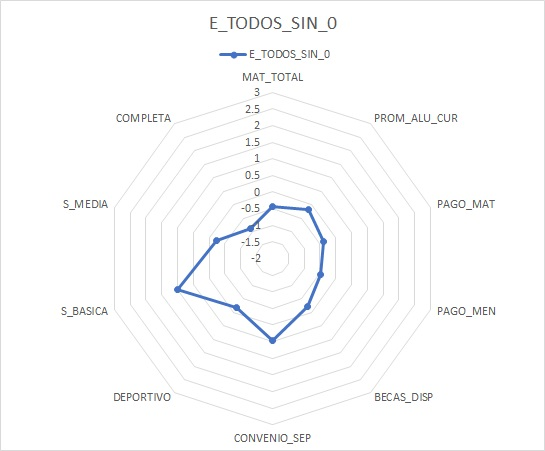
\includegraphics[width=7.3cm]{images/establecimientos/radar_sin_0.jpg}}
  \subfloat[Clúster de establecimientos E\_TODOS\_SIN\_1.]{
   \label{f:radar_estab_sin_1}
    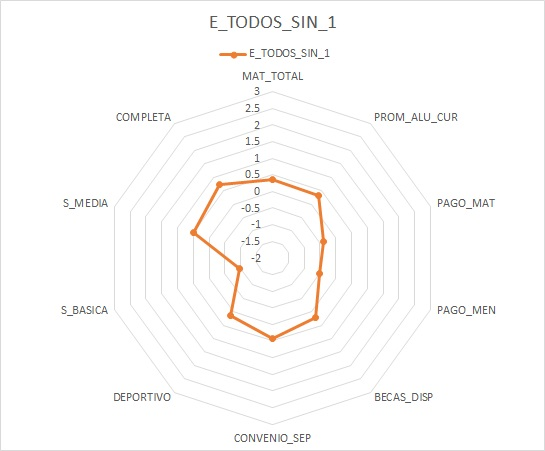
\includegraphics[width=7.3cm]{images/establecimientos/radar_sin_1.jpg}}\hspace{1mm}
  \subfloat[Clúster de establecimientos E\_TODOS\_SIN\_2.]{
   \label{f:radar_estab_sin_2}
    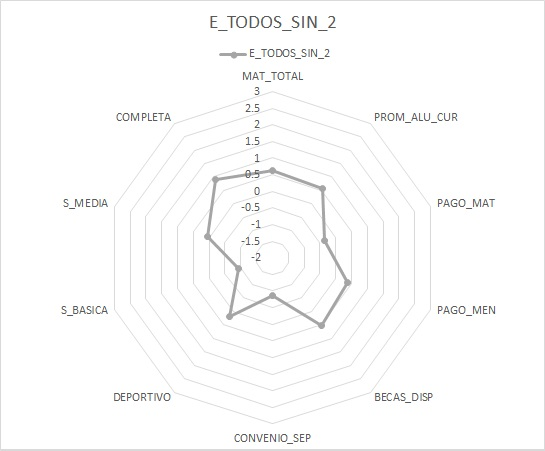
\includegraphics[width=7.3cm]{images/establecimientos/radar_sin_2.jpg}}
  \subfloat[Clúster de establecimientos E\_TODOS\_SIN\_3.]{
   \label{f:radar_estab_sin_3}
    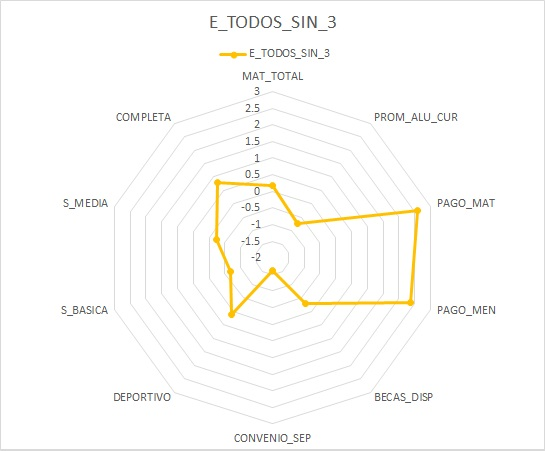
\includegraphics[width=7.3cm]{images/establecimientos/radar_sin_3.jpg}}
 \caption{Promedios de atributos normalizados de establecimientos de la Región Metropolitana.}
 \label{f:radar_estab_sin}
\end{figure}

\begin{table}[H]
\centering
\caption{Clústers de matrículas.}
\label{tab:cl_dependencia_sin}
\begin{tabular}{|c|c|c|c|c|}
\hline
\textbf{Clúster} & \textbf{Municipal} & \textbf{P. Subvencionado} & \textbf{P. Pagado} & \textbf{Corp. Admin. Del.}   \\ \hline
E\_TODOS\_SIN\_0 & 485 & 491 & 1 & 0 \\ \hline
E\_TODOS\_SIN\_1 & 173 & 318 & 0 & 33 \\ \hline
E\_TODOS\_SIN\_2 & 3 & 303 & 2 & 0 \\ \hline
E\_TODOS\_SIN\_3 & 0 & 1 & 258 & 0 \\ \hline
\end{tabular}
\end{table}

De la misma forma se caracterizan los clústers generados al incorporar las variables de relación establecimiento - matrículas, lo que se observa en la figura \ref{f:radar_estab_con} y la tabla \ref{tab:cl_dependencia_con}.

\begin{itemize}
    \item E\_TODOS\_CON\_0: Colegios particulares subvencionados y municipales principalmente de educación básica de matrícula gratuita y mensualidad gratuita o de precio bajo (menor a \$25.000). Poseen convenio SEP e IDE entre 0,5 y 1. Promedio de matrículas: 383, de alumnos por curso: 26 y de becas: 19. La distancia que deben recorrer sus alumnos es de 2.960 metros (percentil 75). El promedio de sobre edad es de 0,524 y 31\% son mayor o igual a 1 año. Estos se distribuyen de la siguiente forma según los años de sobre edad: 74,8\% (1), 18,9\% (2), 5,2\% (3) y 1,1\% (4).
    \item E\_TODOS\_CON\_1: Colegios principalmente particulares subvencionados, municipales y todos los de corporación de administración delegada con educación media o completa, de matrículas y mensualidades gratuitas o de precio bajo (menor a \$25.000). Poseen convenio SEP e IDE entre -0,5 y 0. Promedio de matrículas: 781, de alumnos por curso: 30 y de becas: 58. La distancia que deben recorrer sus alumnos es de 5.204 metros (percentil 75). El promedio de sobre edad es de 0,488 y 32,9\% son mayor o igual a 1 año. Estos se distribuyen de la siguiente forma según los años de sobre edad: 75,1\% (1), 20,6\% (2), 3,9\% (3) y 0,5\% (4).
    \item E\_TODOS\_CON\_2: Colegios particulares subvencionados de educación media o completa con matrículas bajas (menor a \$10.000) y mensualidades medias (\$25.000 - \$100.000). En su mayoría no poseen convenio SEP, nivel deportivo bajo e IDE entre 0 y 1,5. Promedio de matrículas: 895, de alumnos por curso: 32 y de becas: 91. La distancia que deben recorrer sus alumnos es de 5.207 metros (percentil 75). El promedio de sobre edad es de 0,297 y 24\% son mayor o igual a 1 año. Estos se distribuyen de la siguiente forma según los años de sobre edad: 85,3\% (1), 13\% (2), 1,6\% (3) y 0,1\% (4).
    \item E\_TODOS\_CON\_3: Colegios particulares pagados principalmente de educación completa con matrículas y mensualidades elevadas (sobre \$50.000). No poseen convenio SEP y su IDE esta 0,5, pero predominantemente entre 1 y 1,5. Promedio de matrículas: 686, de alumnos por curso: 21 y de becas: 8. La distancia que deben recorrer sus alumnos es de 9.761 metros (percentil 75). El promedio de sobre edad es de 0,488 y 38,1\% son mayor o igual a 1 año. Estos se distribuyen de la siguiente forma según los años de sobre edad: 94,9\% (1), 4,6\% (2), 0,4\% (3) y 0\% (4).
\end{itemize}

\begin{figure}[H]
 \centering
  \subfloat[Clúster de establecimientos E\_TODOS\_CON\_0.]{
   \label{f:radar_estab_con_0}
    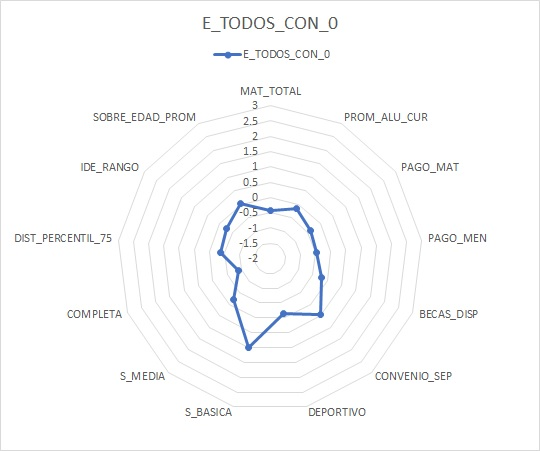
\includegraphics[width=7.3cm]{images/establecimientos/radar_con_0.jpg}}
  \subfloat[Clúster de establecimientos E\_TODOS\_CON\_1.]{
   \label{f:radar_estab_con_1}
    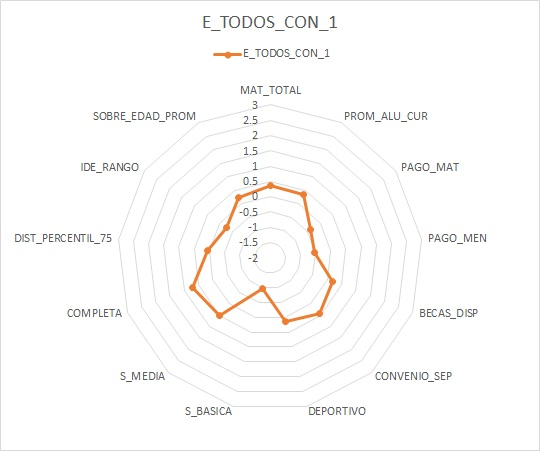
\includegraphics[width=7.3cm]{images/establecimientos/radar_con_1.jpg}}\hspace{1mm}
  \subfloat[Clúster de establecimientos E\_TODOS\_CON\_2.]{
   \label{f:radar_estab_con_2}
    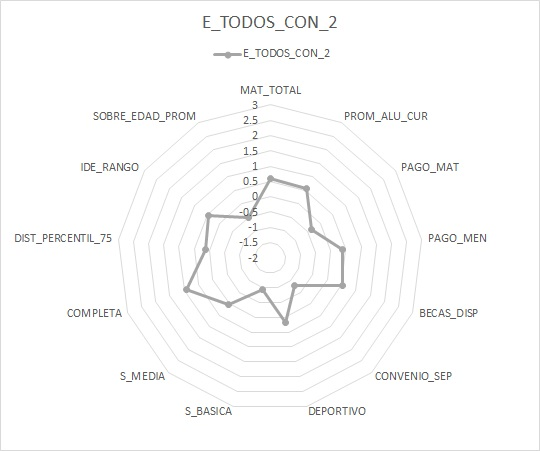
\includegraphics[width=7.3cm]{images/establecimientos/radar_con_2.jpg}}
  \subfloat[Clúster de establecimientos E\_TODOS\_CON\_3.]{
   \label{f:radar_estab_con_3}
    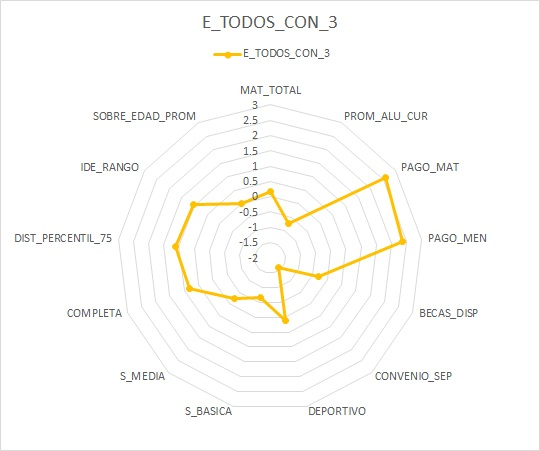
\includegraphics[width=7.3cm]{images/establecimientos/radar_con_3.jpg}}
 \caption{Promedios de atributos normalizados de establecimientos (con atributos relacionales) de la Región Metropolitana.}\
 \label{f:radar_estab_con}
\end{figure}

\begin{table}[H]
\centering
\caption{Clústers de matrículas.}
\label{tab:cl_dependencia_con}
\begin{tabular}{|c|c|c|c|c|}
\hline
\textbf{Clúster} & \textbf{Municipal} & \textbf{P. Subvencionado} & \textbf{P. Pagado} & \textbf{Corp. Admin. Del.}   \\ \hline
E\_TODOS\_CON\_0 & 485 & 489 & 1 & 0 \\ \hlinea
E\_TODOS\_CON\_1 & 173 & 307 & 0 & 33 \\ \hline
E\_TODOS\_CON\_2 & 3 & 316 & 2 & 0 \\ \hline
E\_TODOS\_CON\_3 & 0 & 1 & 258 & 0 \\ \hline
\end{tabular}
\end{table}

Al momento de comparar ambos resultados se puede ver que al incluir las variables de relación los clústers no muestran una gran variación, pero si aumenta el nivel de detalle de cada clúster. A partir de esto se aprecia que los primeros dos clústers son colegios gratuitos o baratos con un IDE bajo que se diferencian entre ellos principalmente por el nivel de educación que imparten. El tercer clúster se diferencia de los anteriores en que su nivel de copago es de un nivel medio al igual que su IDE. Finalmente el cuarto clúster tiene un nivel de copago elevado y un mejor IDE. Un factor que los diferencia a todos es la distancia que recorren sus estudiantes para llegar al establecimiento, ya que desde el primero al cuarto la distancia va en aumento. Finalmente otro punto interesante de analizar es la sobre edad, que en el caso de los colegios mas caros se concentra con un 95\% en un año de sobre edad. En el resto de los clústers el valor fluctúa entre un 75\% y 85\%, y el resto de distribuye de 2 a 4 años de sobre edad.

De manera similar y apoyándose en la figura \ref{f:radar_mat_sin} se caracterizan los clústers de las matrículas, los cuales quedan de la siguiente manera:

\begin{itemize}
  \item M\_TODAS\_SIN\_0: Matrículas de alumnas que son beneficiarias del SEP por pertenecer a Chile solidario o por puntaje de ficha de protección social menor o igual al punto de corte. Tienen una sobre edad promedio de 0,364 y 28,5\% son mayor o igual a 1 año. Estos se distribuyen de la siguiente forma según los años de sobre edad: 76,9\% (1), 18,5\% (2), 4\% (3) y 0,7\% (4).
  \item M\_TODAS\_SIN\_1: Matrículas de alumnos (hombres) que son beneficiarios del SEP por pertenecer a Chile solidario o por puntaje de ficha de protección social menor o igual al punto de corte. Tienen una sobre edad de 0,488 y 36,4\% son mayor o igual a 1 año. Estos se distribuyen de la siguiente forma según los años de sobre edad: 72,5\% (1), 21,5\% (2), 5,2\% (3) y 0,9\% (4).
  \item M\_TODAS\_SIN\_2: Matrículas de alumnas que no son beneficiarias SEP. Tienen una sobre edad de 0,284 y 25,7\% son mayor o igual a 1 año. Estos se distribuyen de la siguiente forma según los años de sobre edad: 90,2\% (1), 8,7\% (2), 1\% (3) y 0,1\% (4).

  \item M\_TODAS\_SIN\_3: Matrículas de alumnos (hombres) que no son beneficiarios SEP. Tienen una sobre edad de 0,365 y 32\% son mayor o igual a 1 año. Estos se distribuyen de la siguiente forma según los años de sobre edad: 87,\% (1), 11,1\% (2), 1,5\% (3) y 0,1\% (4).
\end{itemize}

\begin{figure}[H]
 \centering
  \subfloat[Clúster de matrículas M\_TODAS\_SIN\_0.]{
   \label{f:radar_mat_sin_0}
    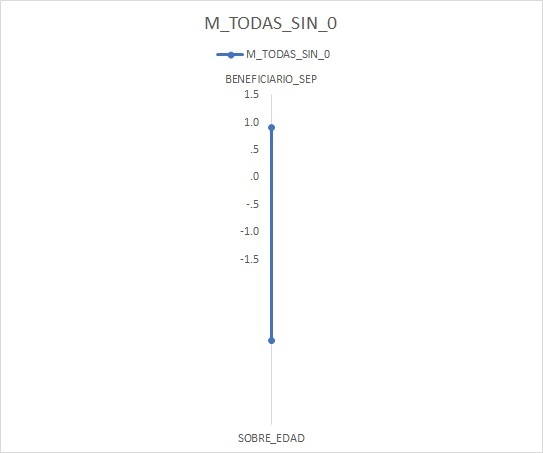
\includegraphics[width=7.3cm]{images/matriculas/radar_mat_sin_0.jpg}}
  \subfloat[Clúster de matrículas M\_TODAS\_SIN\_1.]{
   \label{f:radar_mat_sin_1}
    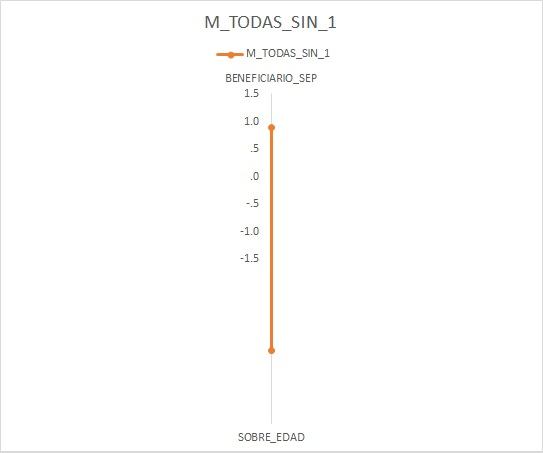
\includegraphics[width=7.3cm]{images/matriculas/radar_mat_sin_1.jpg}}\hspace{1mm}
  \subfloat[Clúster de matrículas M\_TODAS\_SIN\_2.]{
   \label{f:radar_mat_sin_2}
    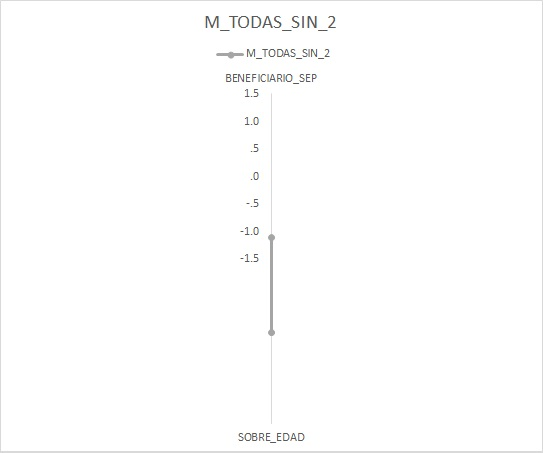
\includegraphics[width=7.3cm]{images/matriculas/radar_mat_sin_2.jpg}}
  \subfloat[Clúster de matrículas M\_TODAS\_SIN\_3.]{
   \label{f:radar_mat_sin_3}
    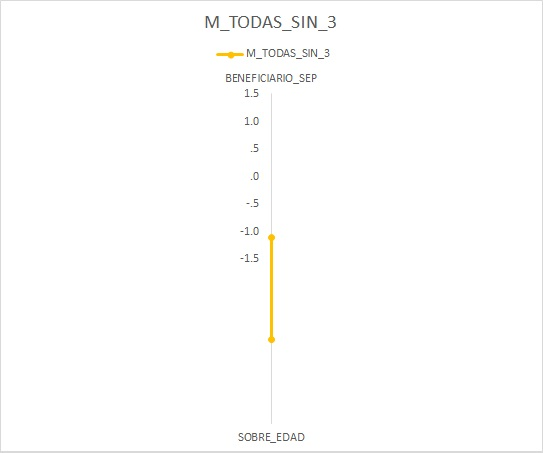
\includegraphics[width=7.3cm]{images/matriculas/radar_mat_sin_3.jpg}}
 \caption{Promedios de atributos normalizados de matrículas de la Región Metropolitana.}\
 \label{f:radar_mat_sin}
\end{figure}

Y según la figura \ref{f:radar_mat_con} los clústers de matrículas incluyendo las variables de relación establecimiento - matrícula quedan caracterizados de la siguiente manera:

\begin{itemize}
  \item M\_TODAS\_CON\_0: Matrículas de alumnos (hombres) que son beneficiarios del SEP por pertenecer a Chile solidario o por puntaje ficha de protección social menor o igual al punto de corte. Asisten principalmente a colegios de matrícula y mensualidad gratuita. Tienen una sobre edad de 0,492 y 36,7\% son mayor o igual a 1 año. Estos se distribuyen de la siguiente forma según los años de sobre edad: 72,4\% (1), 21,6\% (2), 5,1\% (3) y 0,9\% (4). La distancia que deben recorrer es de 4.939 metros (percentil 75).  
  \item M\_TODAS\_CON\_1: Matrículas de alumnas que son beneficiarias del SEP por pertenecer a Chile solidario o por puntaje ficha de protección social menor o igual al punto de corte. Asisten principalmente a colegios de matrícula y mensualidad gratuita. Tienen una sobre edad de 0,370 y 28,9\% son mayor o igual a 1 año. Estos se distribuyen de la siguiente forma según los años de sobre edad: 76,7\% (1), 18,7\% (2), 3,9\% (3) y 0,7\% (4). La distancia que deben recorrer es de 4.711 metros (percentil 75).
  \item M\_TODAS\_CON\_2: Matrículas de alumnos (hombres y mujeres) que no son beneficiarios del SEP, que asisten principalmente a colegios con matrícula gratuita y mensualidad entre los \$10.000 y \$100.000. Tienen una sobre edad de 0,270 y 23,4\% son mayor o igual a 1 año. Estos se distribuyen de la siguiente forma según los años de sobre edad: 85,9\% (1), 12,4\% (2), 1,6\% (3) y 0,1\% (4). La distancia que deben recorrer es de 5.912 metros (percentil 75).
  \item M\_TODAS\_CON\_3: Matrículas de alumnos (hombres y mujeres) que no son beneficiarios del SEP, que asisten principalmente a colegios con matrícula y mensualidad mayores a \$100.000.  Tienen una sobre edad de 0,401 y 38,1\% son mayor o igual a 1 año. Estos se distribuyen de la siguiente forma según los años de sobre edad: 94,9\% (1), 4,6\% (2), 0,4\% (3) y 0\% (4). La distancia promedio que deben recorrer es de 4.911 (percentil 75).
\end{itemize}

\begin{figure}[H]
 \centering
  \subfloat[Clúster de matrículas M\_TODAS\_CON\_0.]{
   \label{f:radar_mat_con_0}
    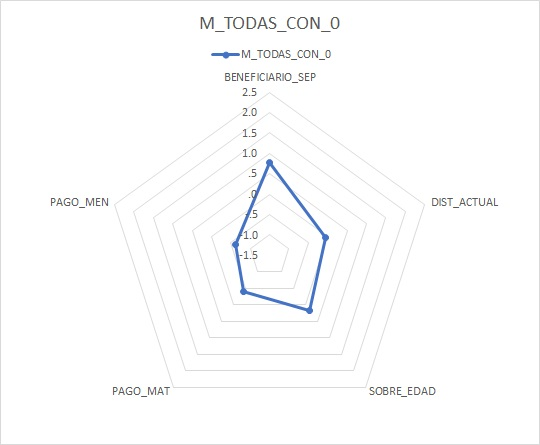
\includegraphics[width=7.3cm]{images/matriculas/radar_mat_con_0.jpg}}
  \subfloat[Clúster de matrículas M\_TODAS\_CON\_1.]{
   \label{f:radar_mat_con_1}
    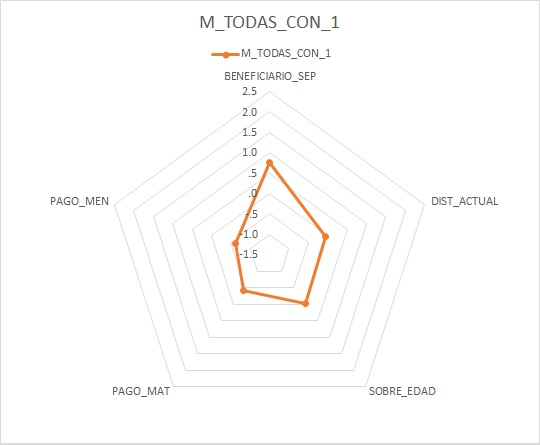
\includegraphics[width=7.3cm]{images/matriculas/radar_mat_con_1.jpg}}\hspace{1mm}
  \subfloat[Clúster de matrículas M\_TODAS\_CON\_2.]{
   \label{f:radar_mat_con_2}
    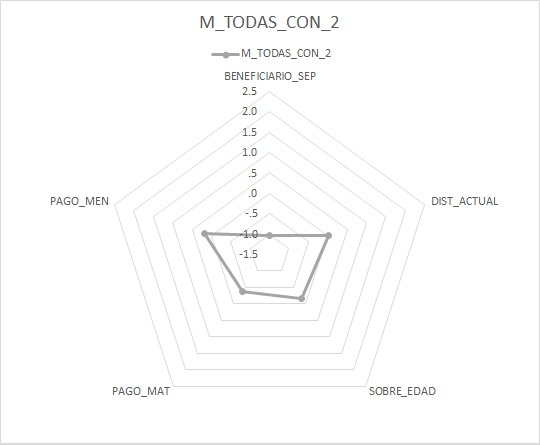
\includegraphics[width=7.3cm]{images/matriculas/radar_mat_con_2.jpg}}
  \subfloat[Clúster de matrículas M\_TODAS\_CON\_3.]{
   \label{f:radar_mat_con_3}
    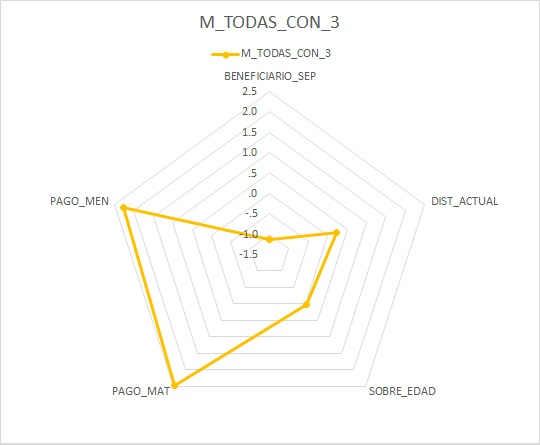
\includegraphics[width=7.3cm]{images/matriculas/radar_mat_con_3.jpg}}
 \caption{Promedios de atributos normalizados de matrículas (con atributos relacionales) de la Región Metropolitana.}\
 \label{f:radar_mat_con}
\end{figure}

Al comparar los resultados obtenidos con y sin las variables de relación establecimiento - matrículas, se puede notar que al no utilizar dichas variables los clústers se dividen principalmente por género y por el acceso que tienen al SEP. Al incorporar las variables de copago y distancia a los establecimientos, los primeros clústers no muestran cambios significativos, siendo los últimos dos los que presentan mayores diferencias en comparación a los sin variables del relación. Dichos grupos dejan de ser excluyentes por género y el factor que predomina es el nivel de copago que estos presentan. 

Con los clústers ya realizados, y sus respectivas geolocalizaciones, se superponen sobre el mapa de grupo socioeconómico de la Región Metropolitana obteniendo los mapas de las figuras \ref{f:mapas_estab_sin_gse} y \ref{f:mapas_estab_con_gse}. Por ser tan similares los resultados de ambas pruebas (con y sin variables de relación) sus diferencias son imperceptibles en los mapas generados. En el mapa de la figura \ref{f:mapa_estab_sin_0} se aprecia que los establecimientos se distribuyen uniformemente por el área matropolitana, exceptuando la zona oriente (salvo en algunos casos). Concentrándose mayoritariamente en las zonas anaranjadas, los cuales pertenecen a los deciles del 3 al 7. De la misma forma en la figura \ref{f:mapa_estab_sin_1} los establecimientos se distribuyen de manera uniforme sobre las zonas anaranjadas, con la diferencia de que disminuye su cardinalidad. En la figura \ref{f:mapa_estab_sin_2} los colegios se encuentran distribuidos en las zonas que comprenden los deciles del 4 al 7, pero estos se encuentran agrupados en diferentes sectores de la zona que comprenden. Finalmente el último clúster de colegios, representado en la figura \ref{f:mapa_estab_sin_3}, ubica sus establecimientos en la zona oriente de la capital (deciles del 8 al 10), la cual corresponde al sector con mayor ingreso per cápita. 

\begin{figure}[H]
 \centering
  \subfloat[Establecimientos clúster E\_TODOS\_SIN\_0.]{
   \label{f:mapa_estab_sin_0}
    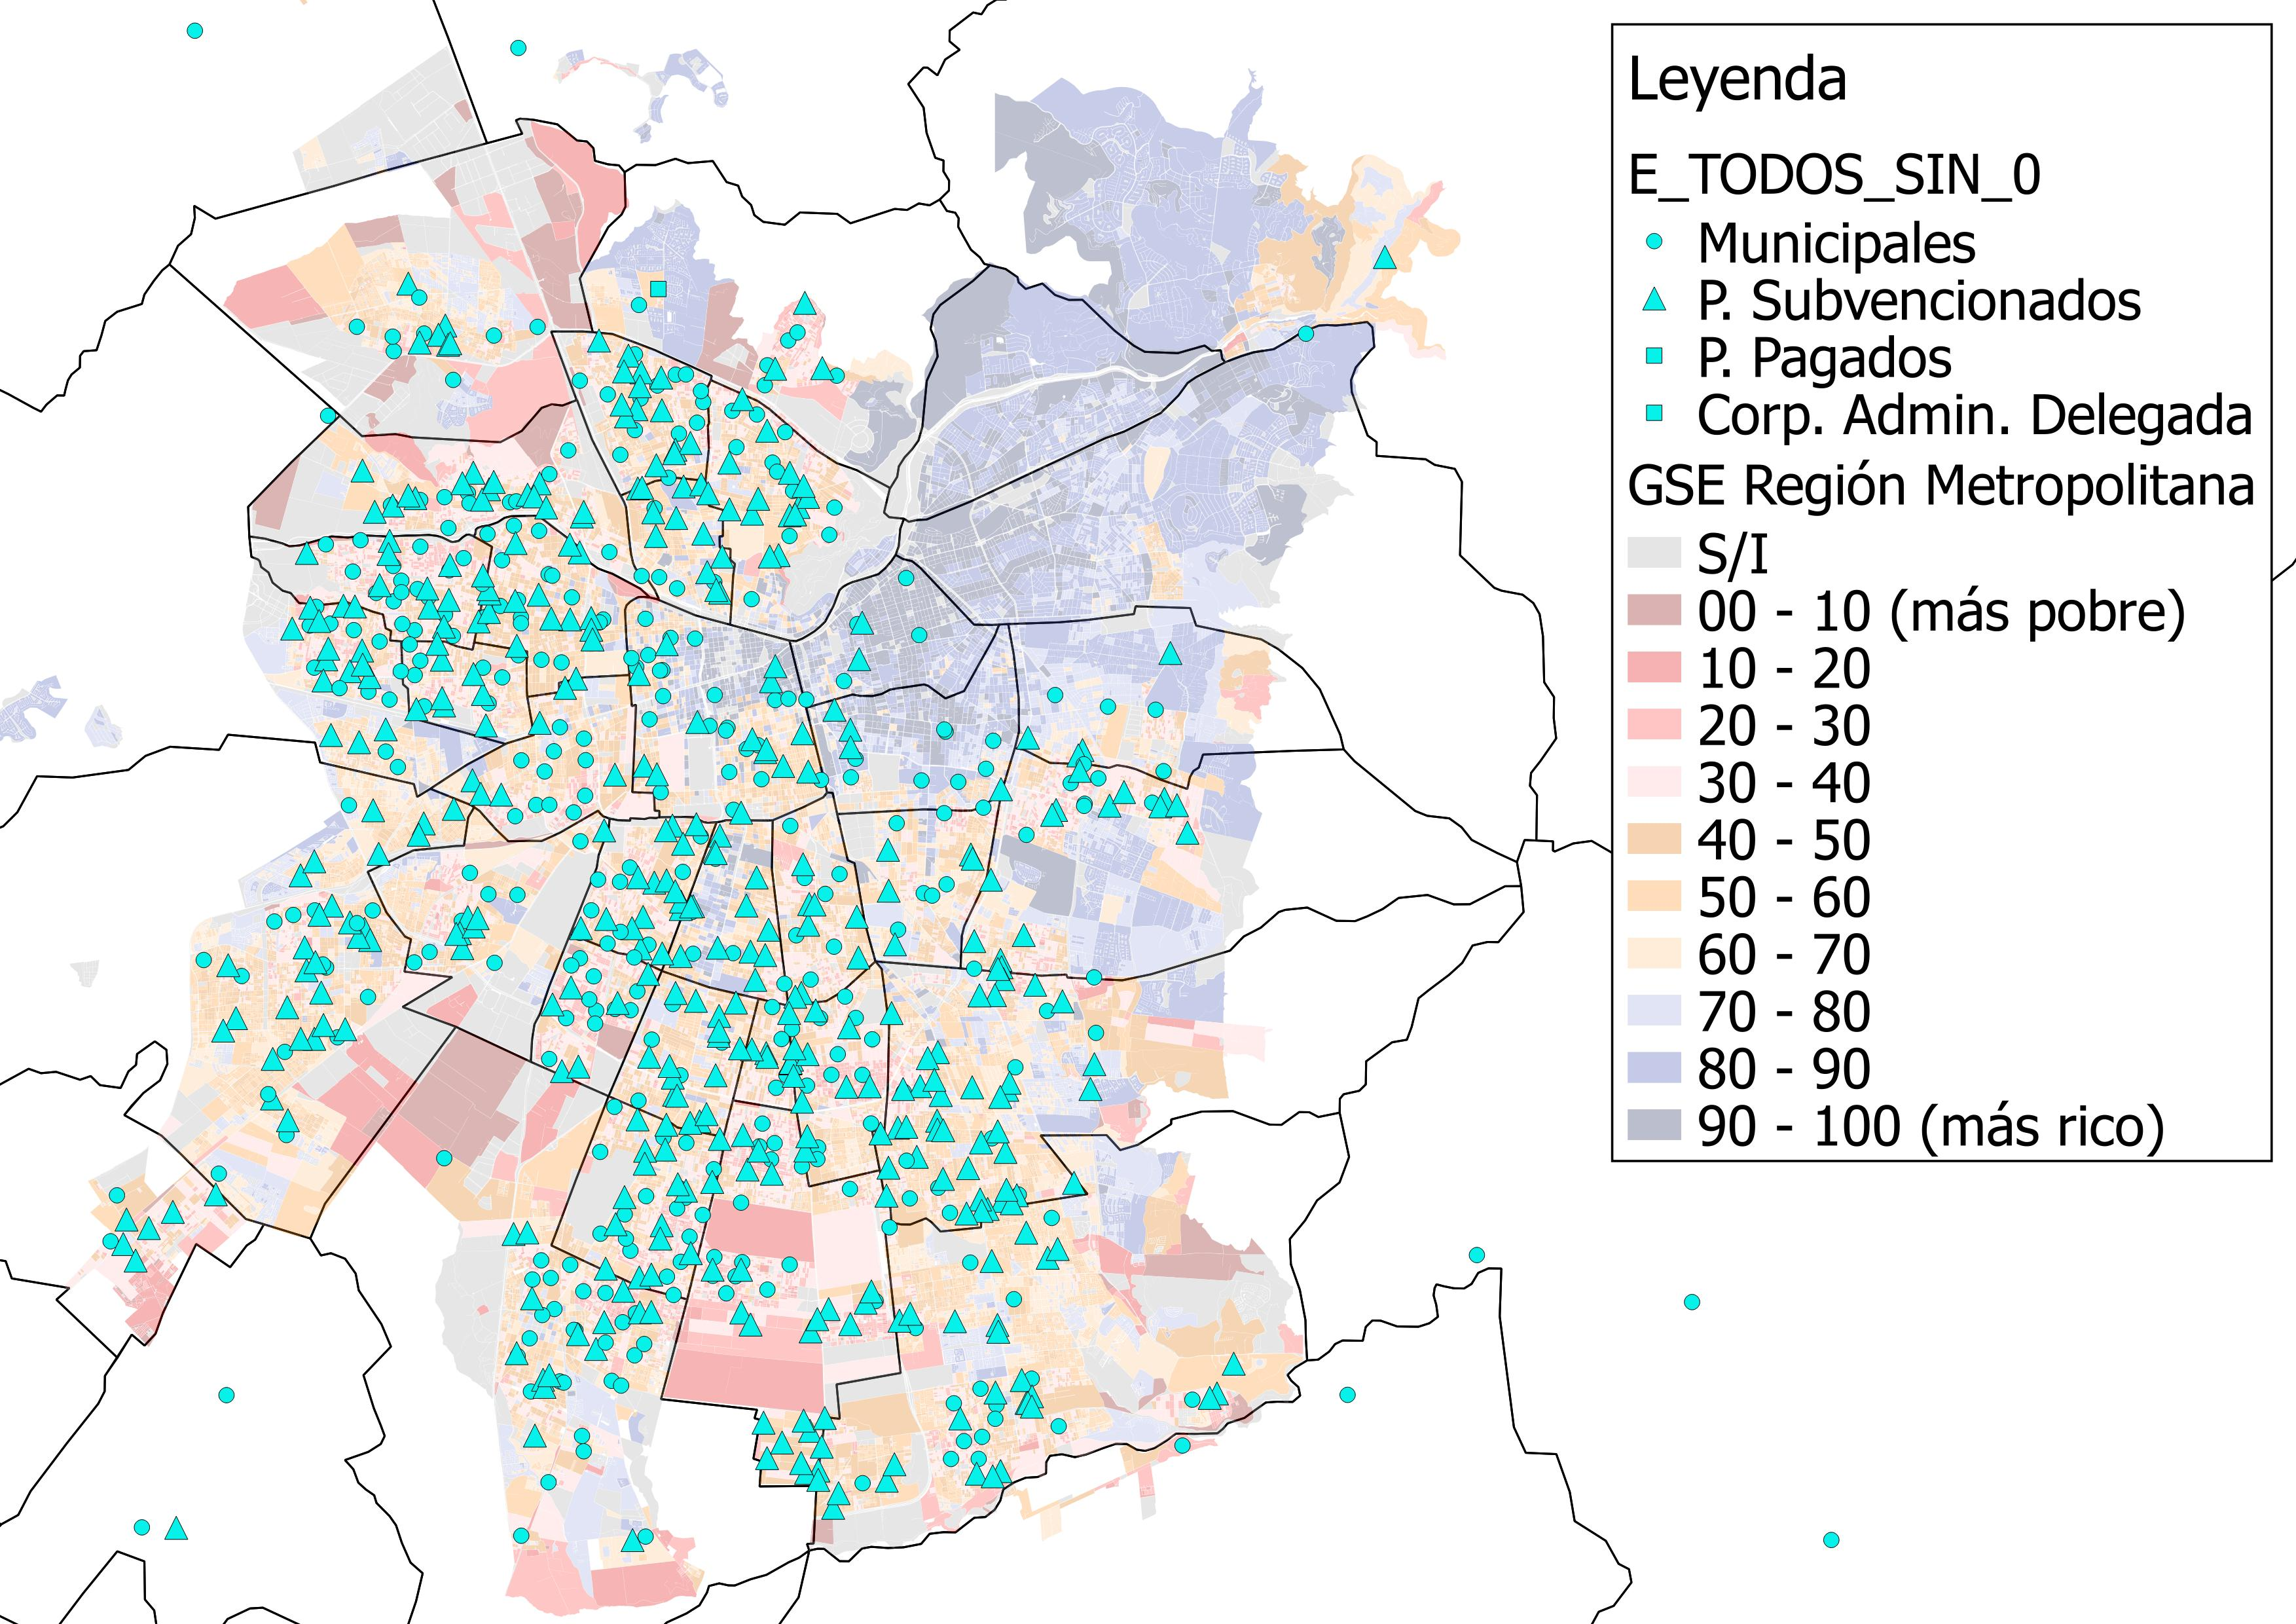
\includegraphics[width=7.5cm]{images/establecimientos/E_TODOS_SIN_0.jpg}}
  \subfloat[Establecimientos clúster E\_TODOS\_SIN\_1.]{
   \label{f:mapa_estab_sin_1}
    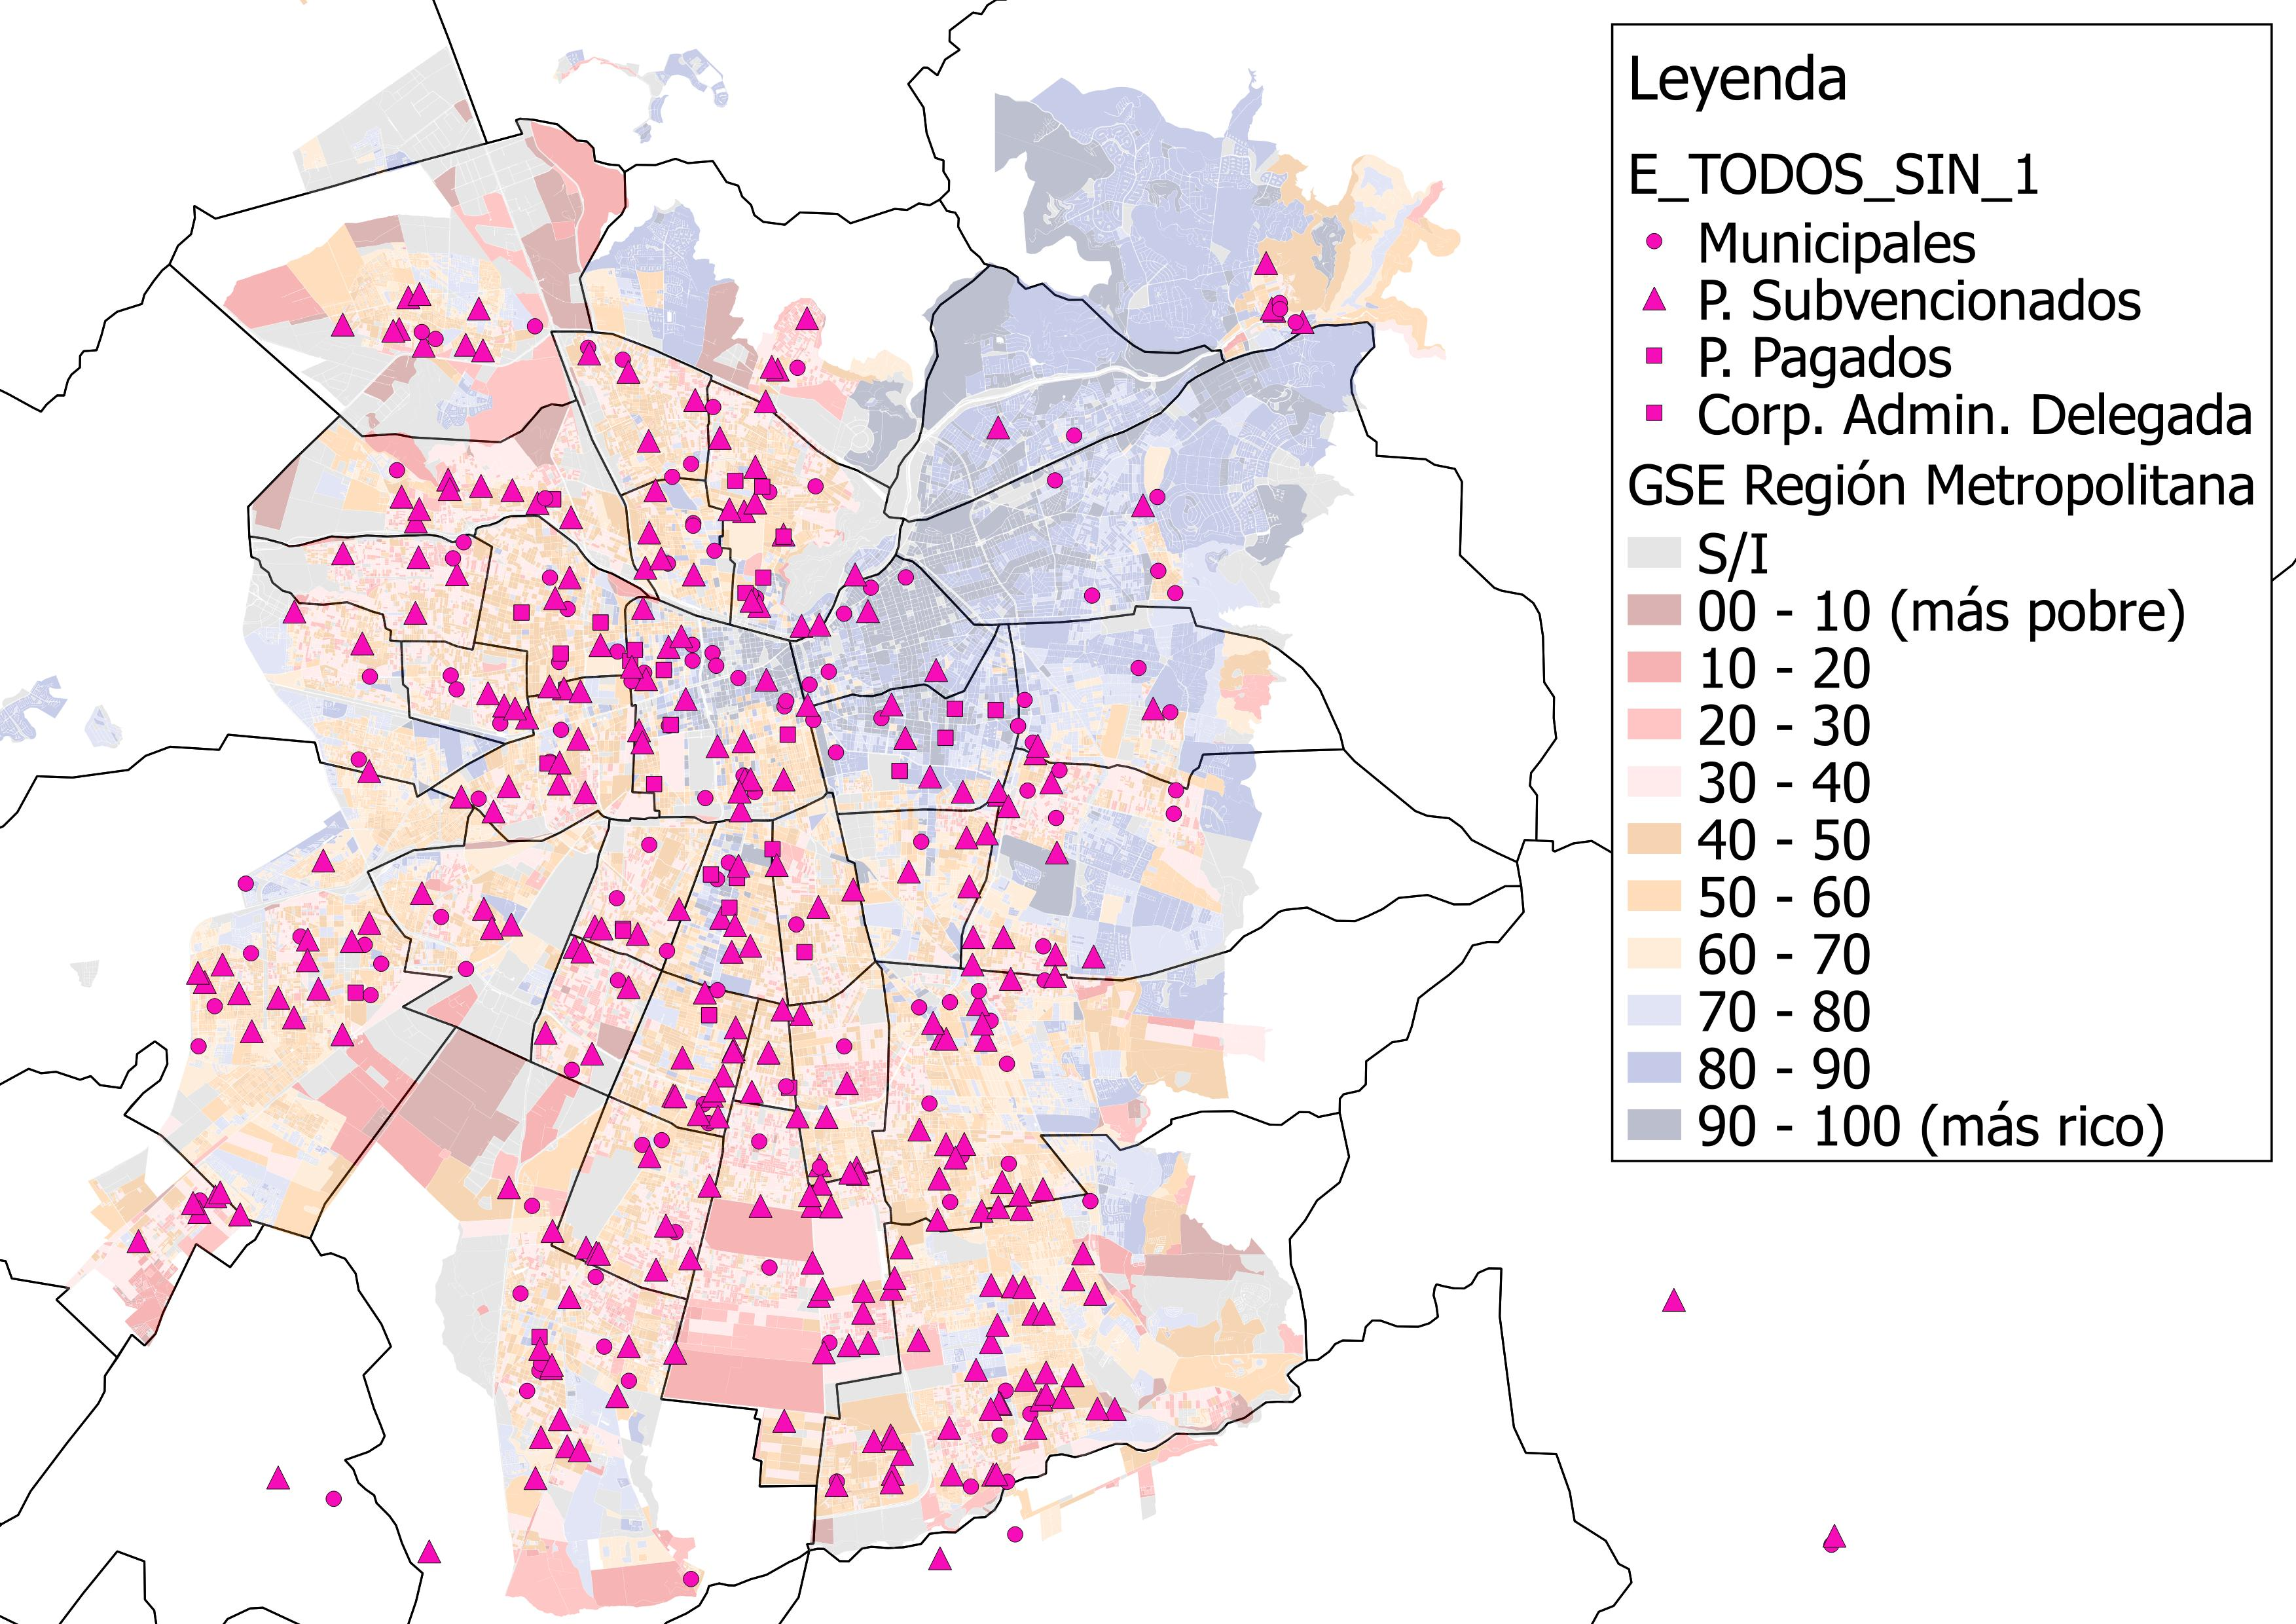
\includegraphics[width=7.5cm]{images/establecimientos/E_TODOS_SIN_1.jpg}}\hspace{1mm}
  \subfloat[Establecimientos clúster E\_TODOS\_SIN\_2.]{
   \label{f:mapa_estab_sin_2}
    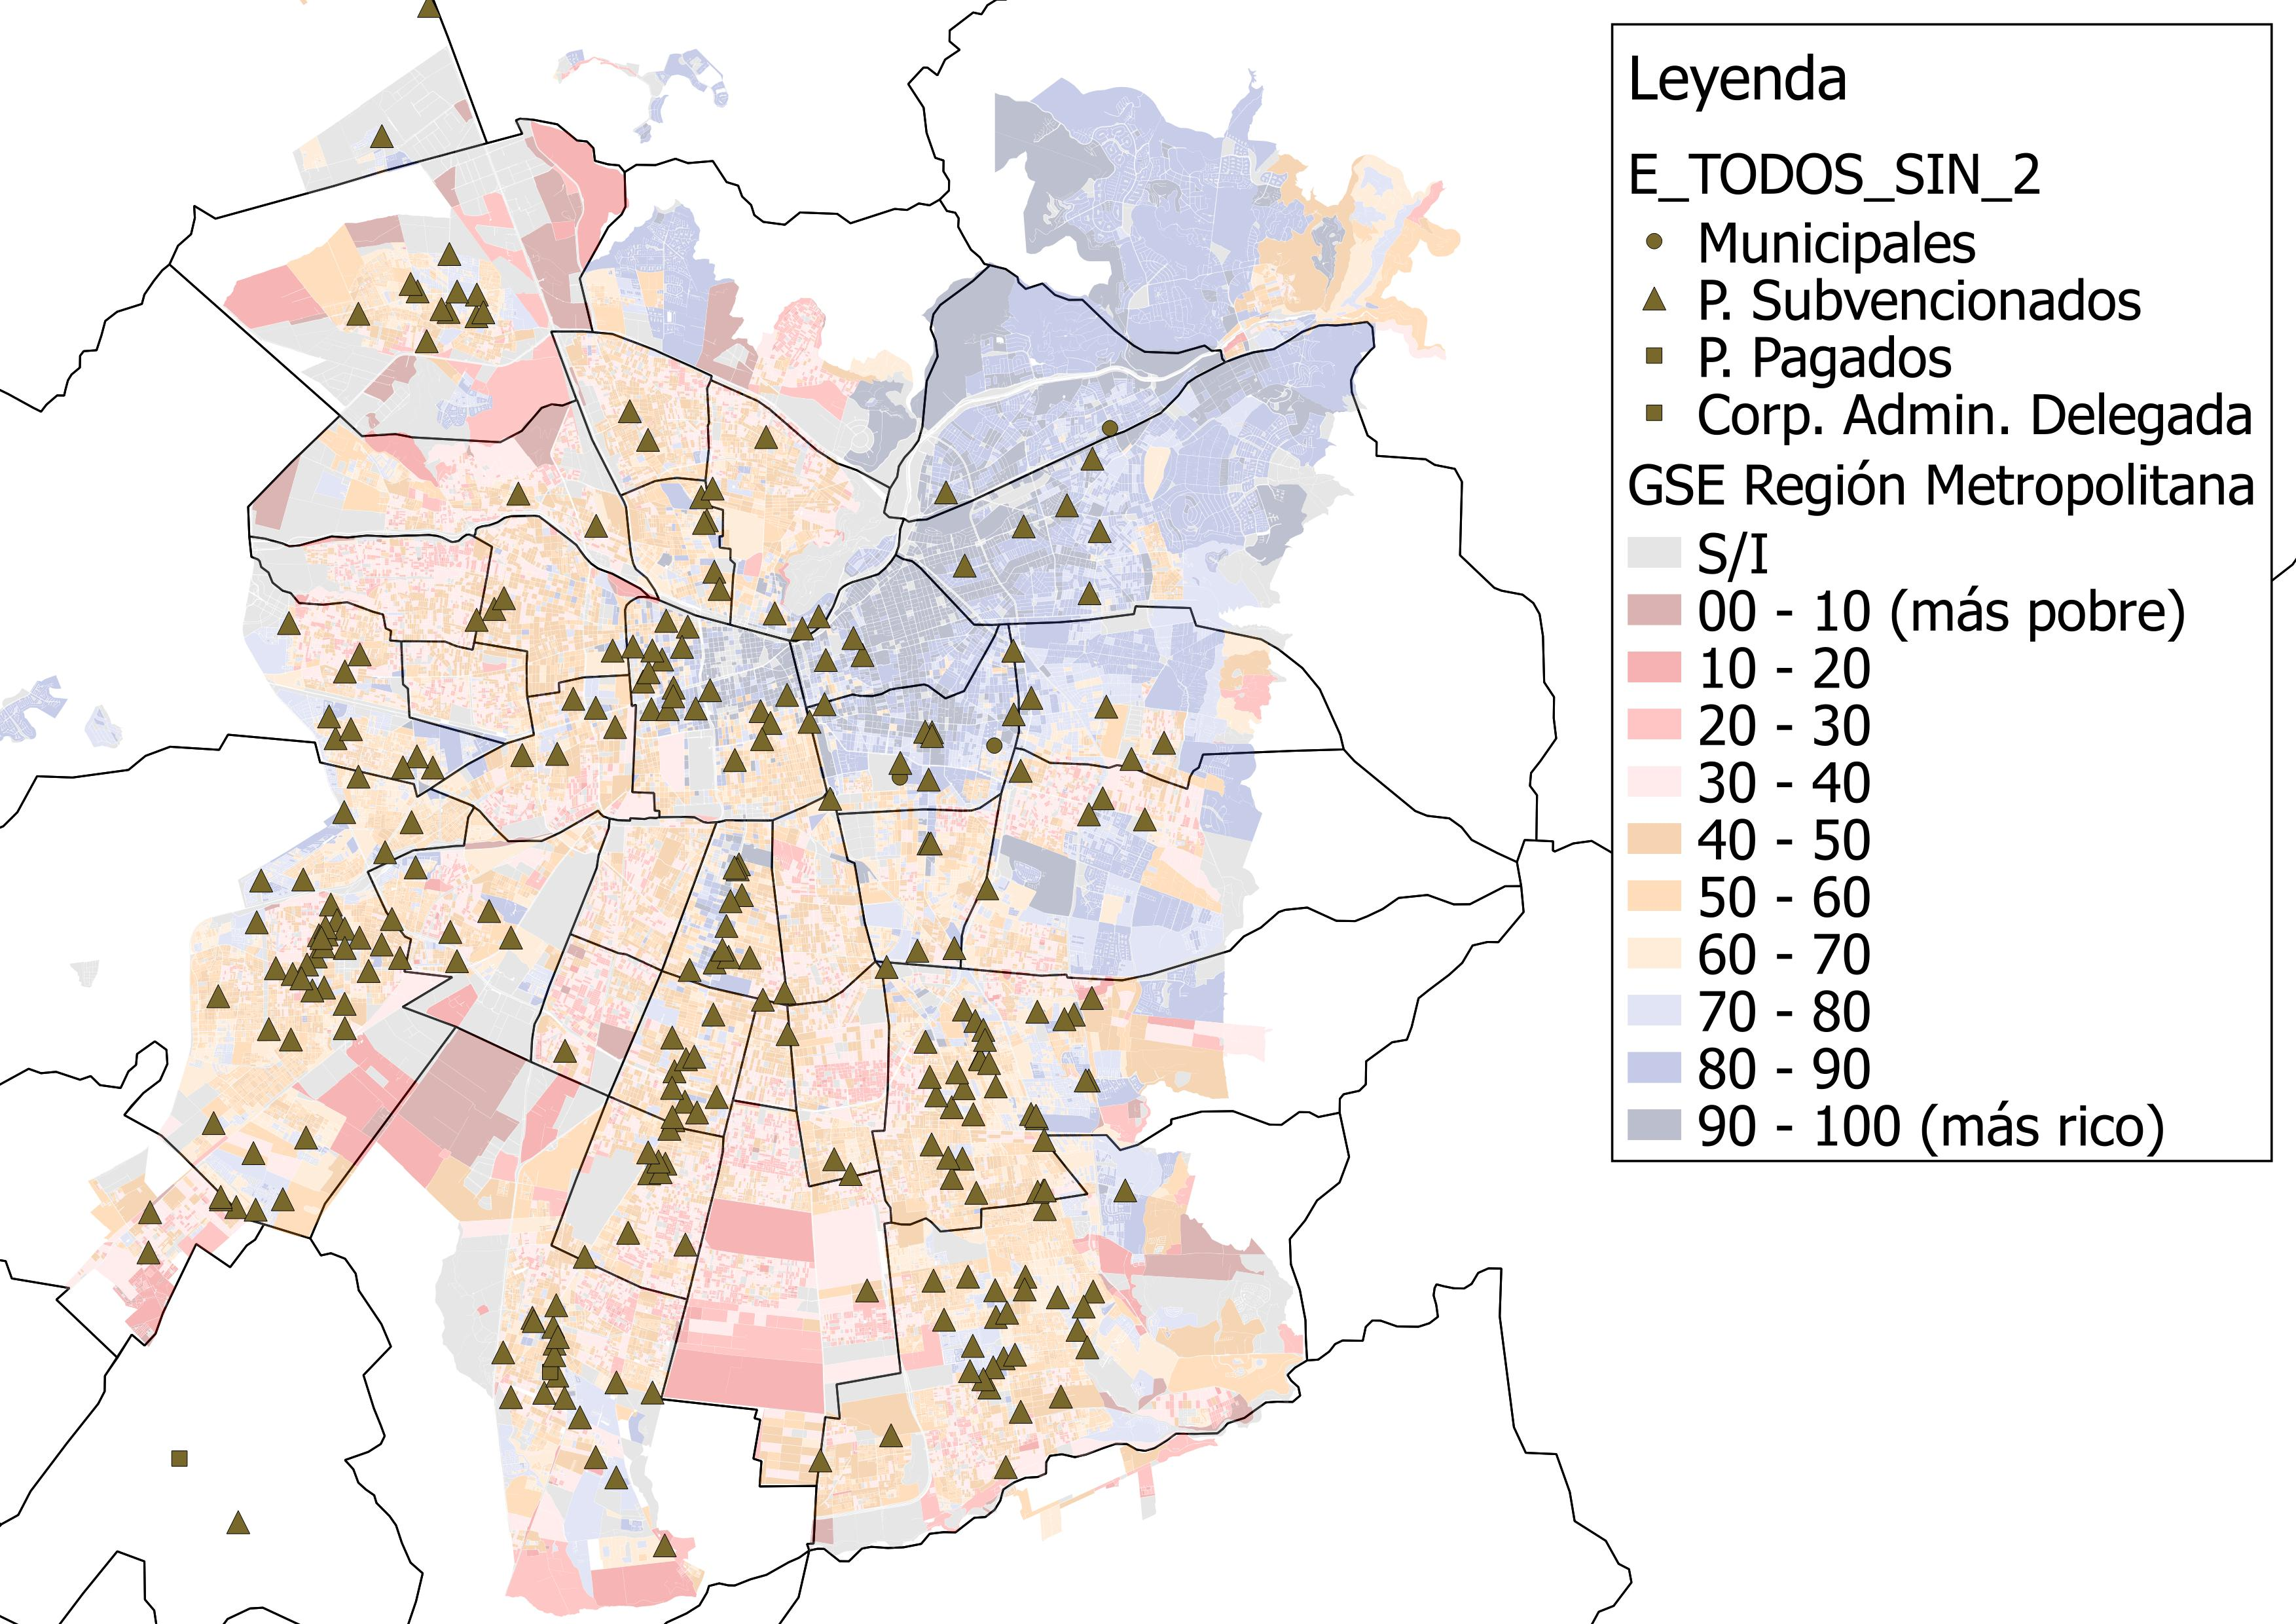
\includegraphics[width=7.5cm]{images/establecimientos/E_TODOS_SIN_2.jpg}}
  \subfloat[Establecimientos clúster E\_TODOS\_SIN\_3.]{
   \label{f:mapa_estab_sin_3}
    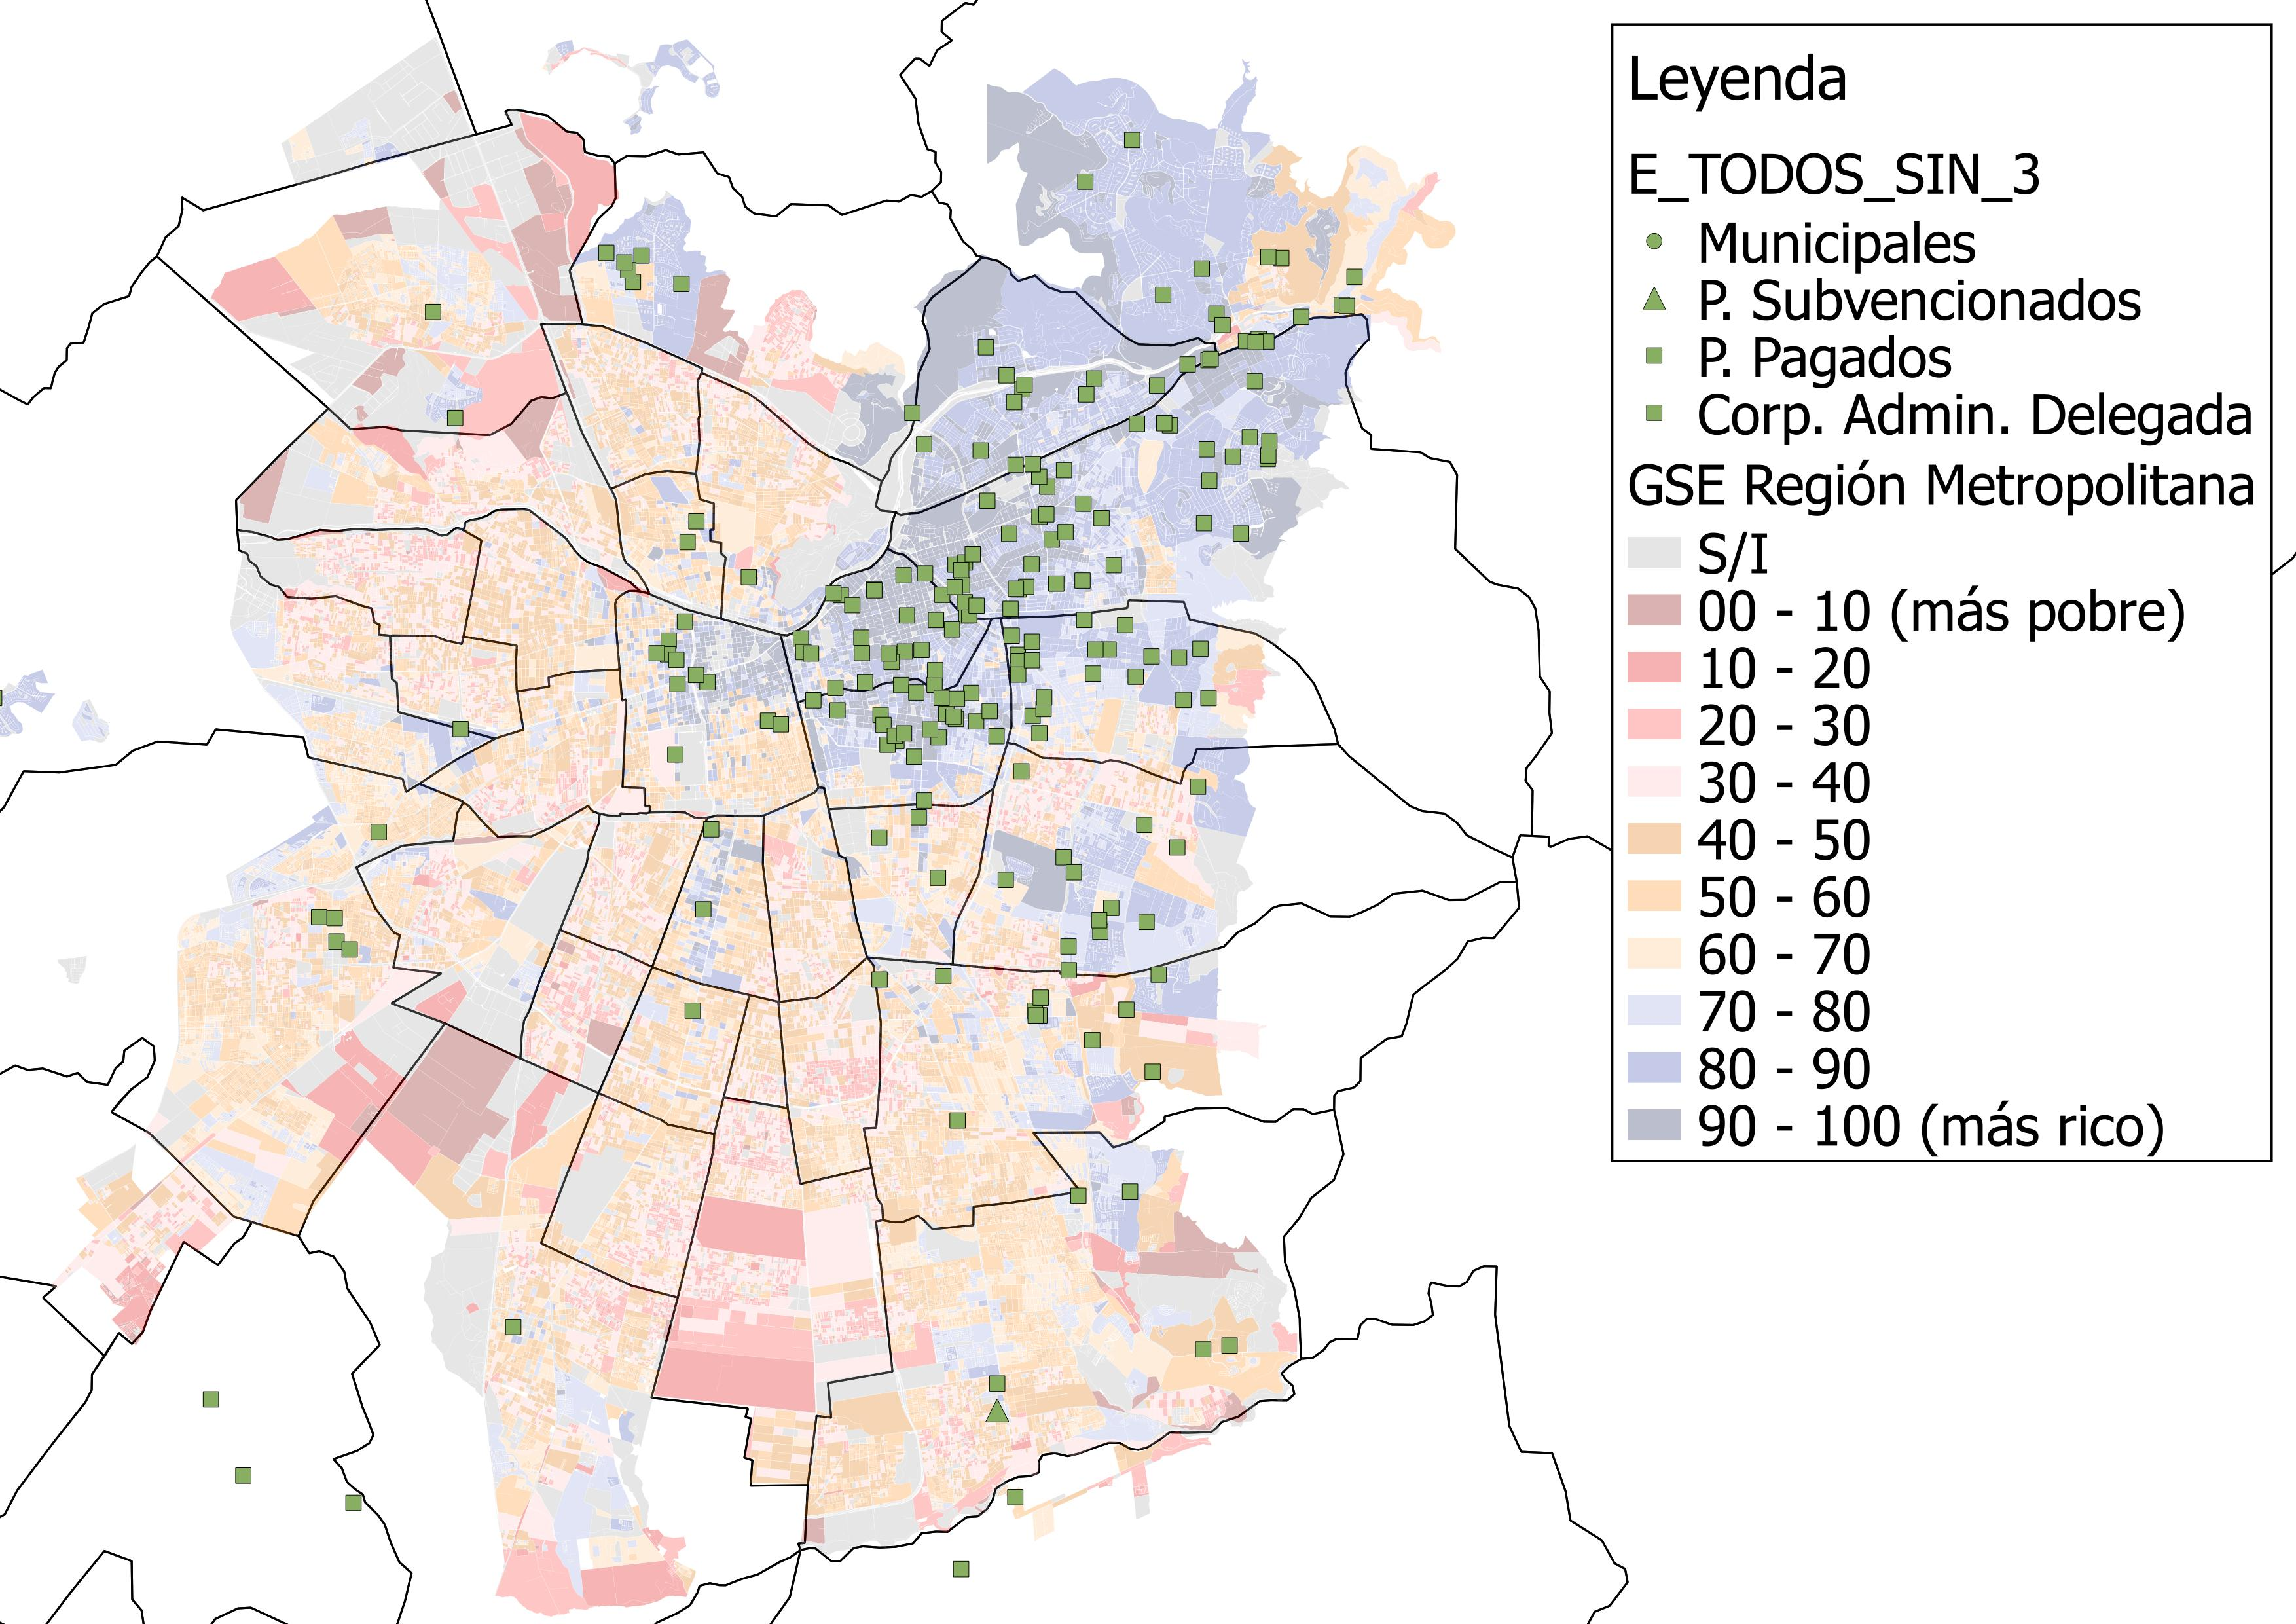
\includegraphics[width=7.5cm]{images/establecimientos/E_TODOS_SIN_3.jpg}}
 \caption{Mapas de clústers de establecimientos sobre mapa GSE de la Región Metropolitana.}
 \label{f:mapas_estab_sin_gse}
\end{figure}

Además de lo anteriormente señalado para cada clúster, se puede indicar que en su gran mayoría los establecimientos educacionales de la Región Metropolitana se encuentran en el área metropolitana y particularmente son en mayor parte del primer clúster.

Para el caso de la figura \ref{f:mapas_estab_con_gse} el análisis es similar al realizado anteriormente, debido a que el considerar o no las variables de relación establecimiento - matrícula no generan un gran impacto en la distribución de los clústers generados sin incluir dichas variables.

\begin{figure}[H]
 \centering
  \subfloat[Establecimientos clúster E\_TODOS\_CON\_0.]{
   \label{f:mapa_estab_con_0}
    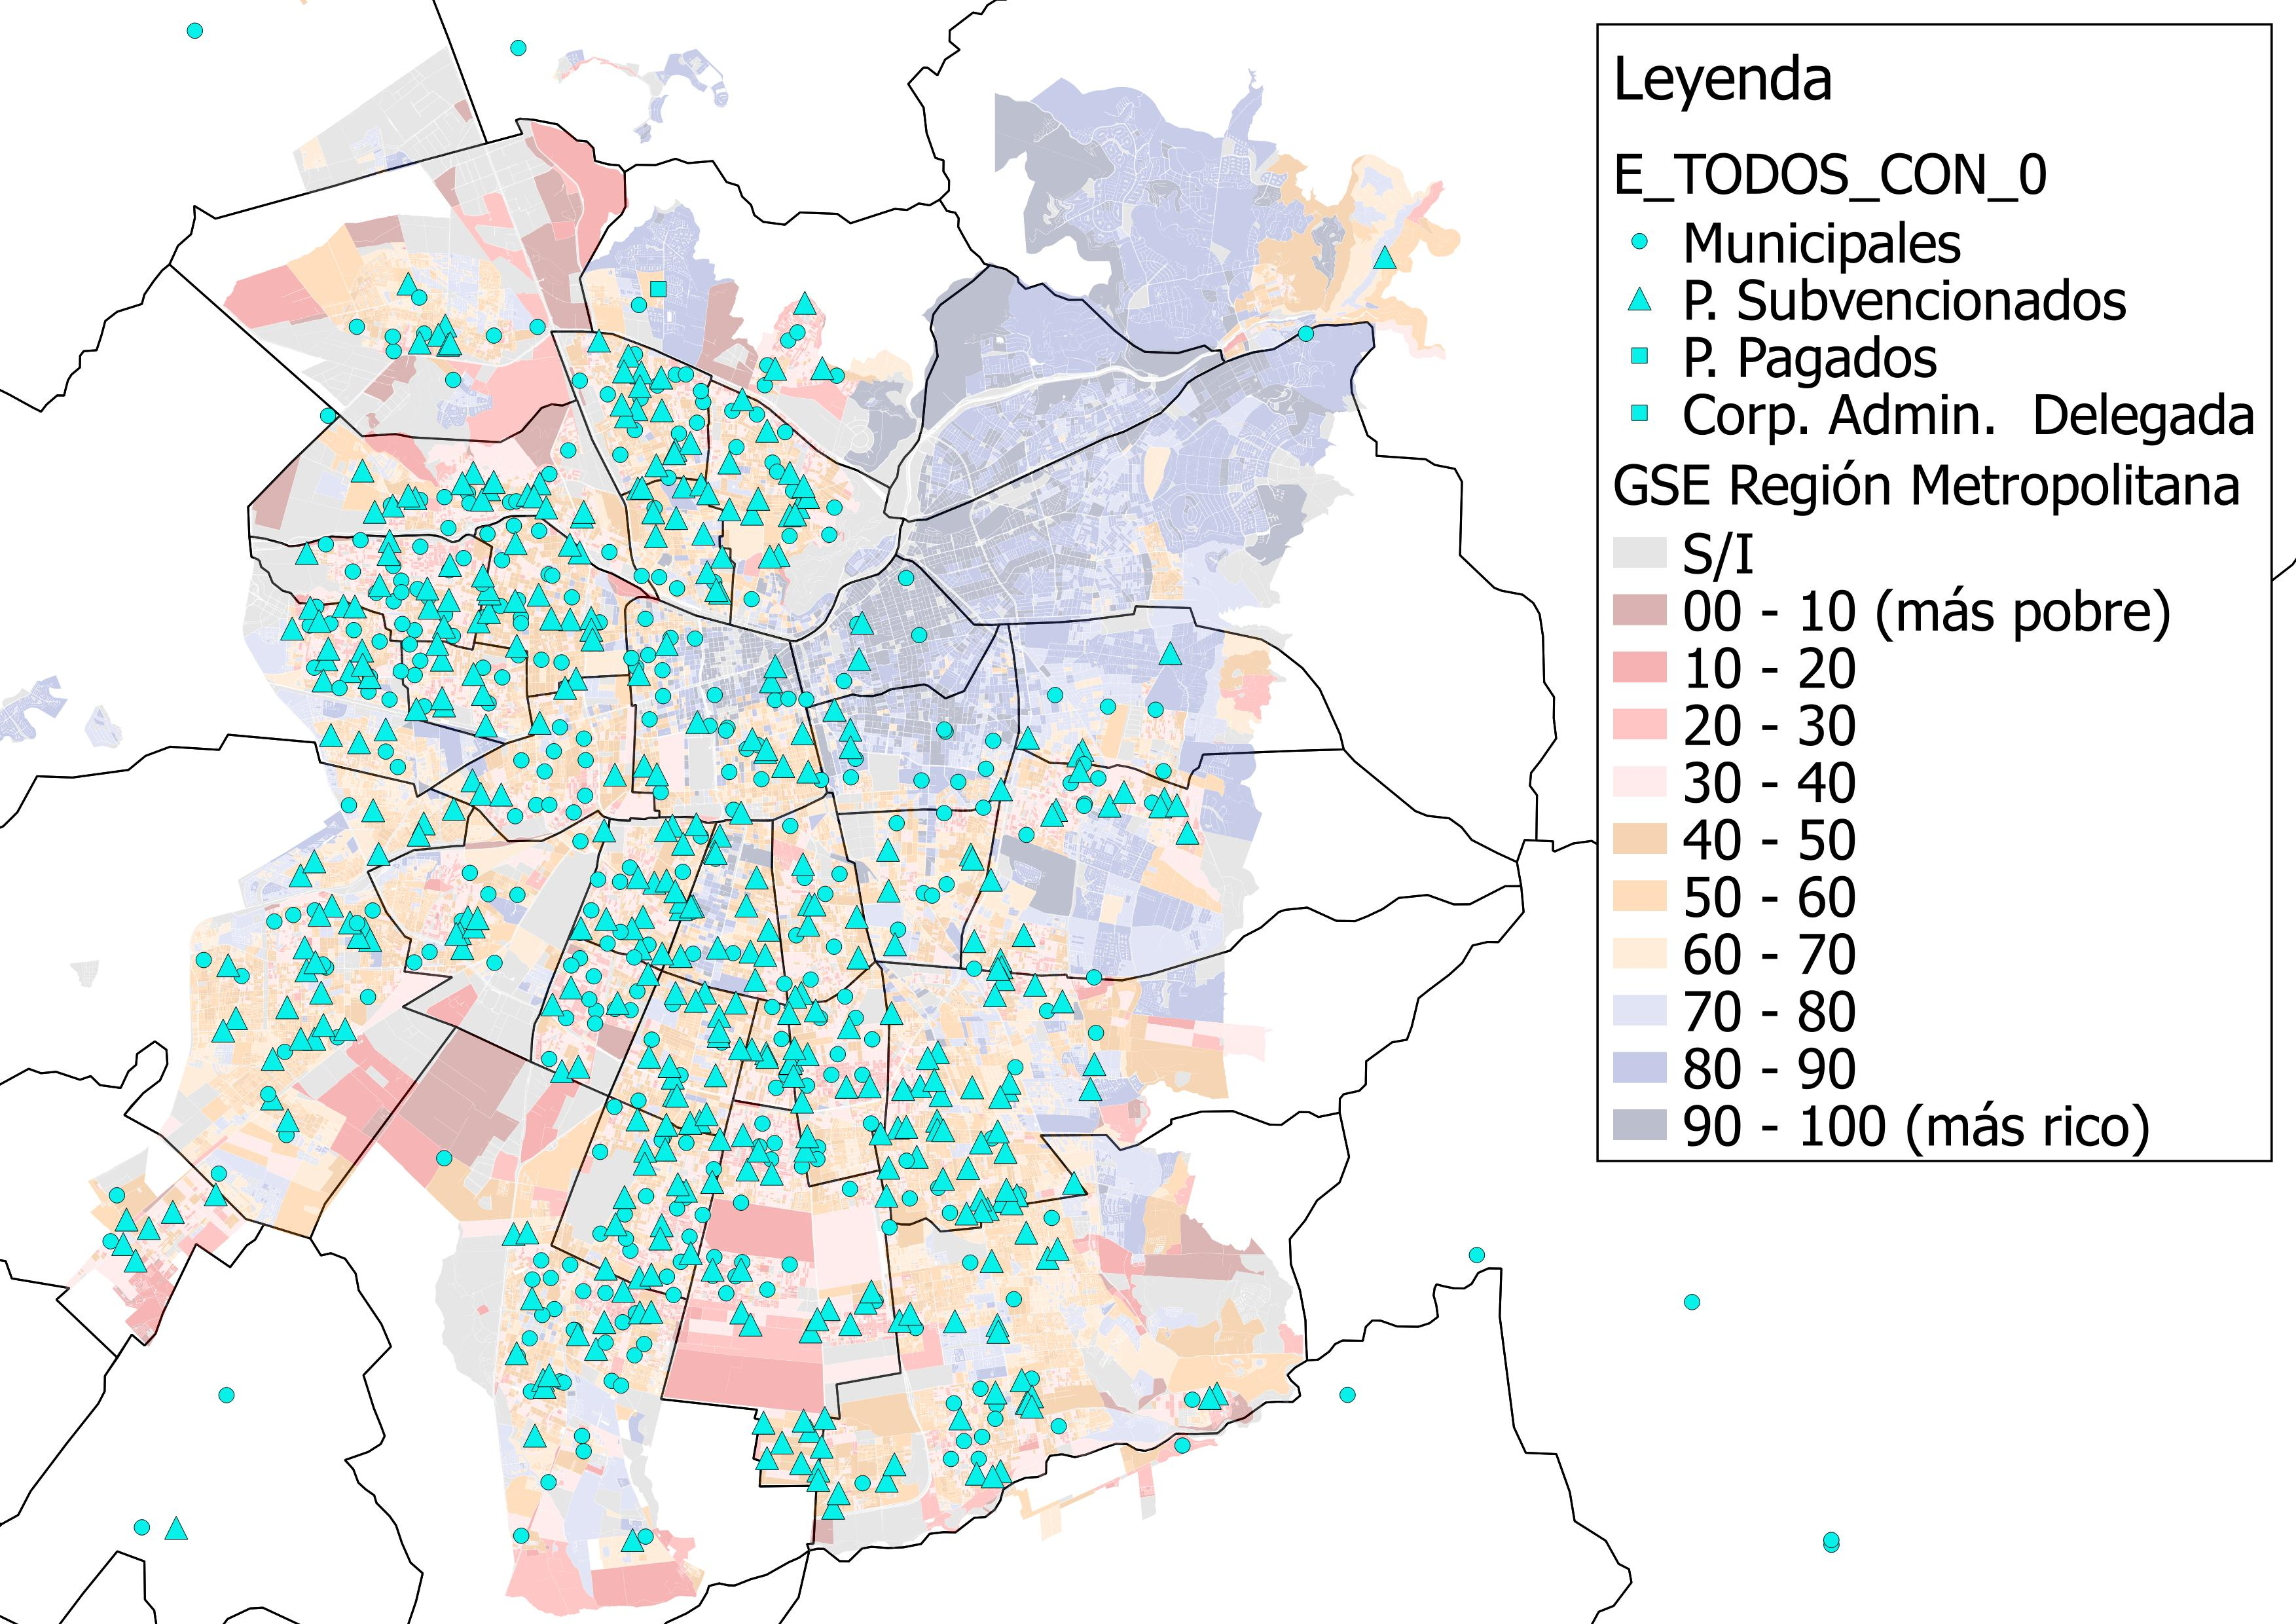
\includegraphics[width=7.5cm]{images/establecimientos/E_TODOS_CON_0.jpg}}
  \subfloat[Establecimientos clúster E\_TODOS\_CON\_1.]{
   \label{f:mapa_estab_con_0}
    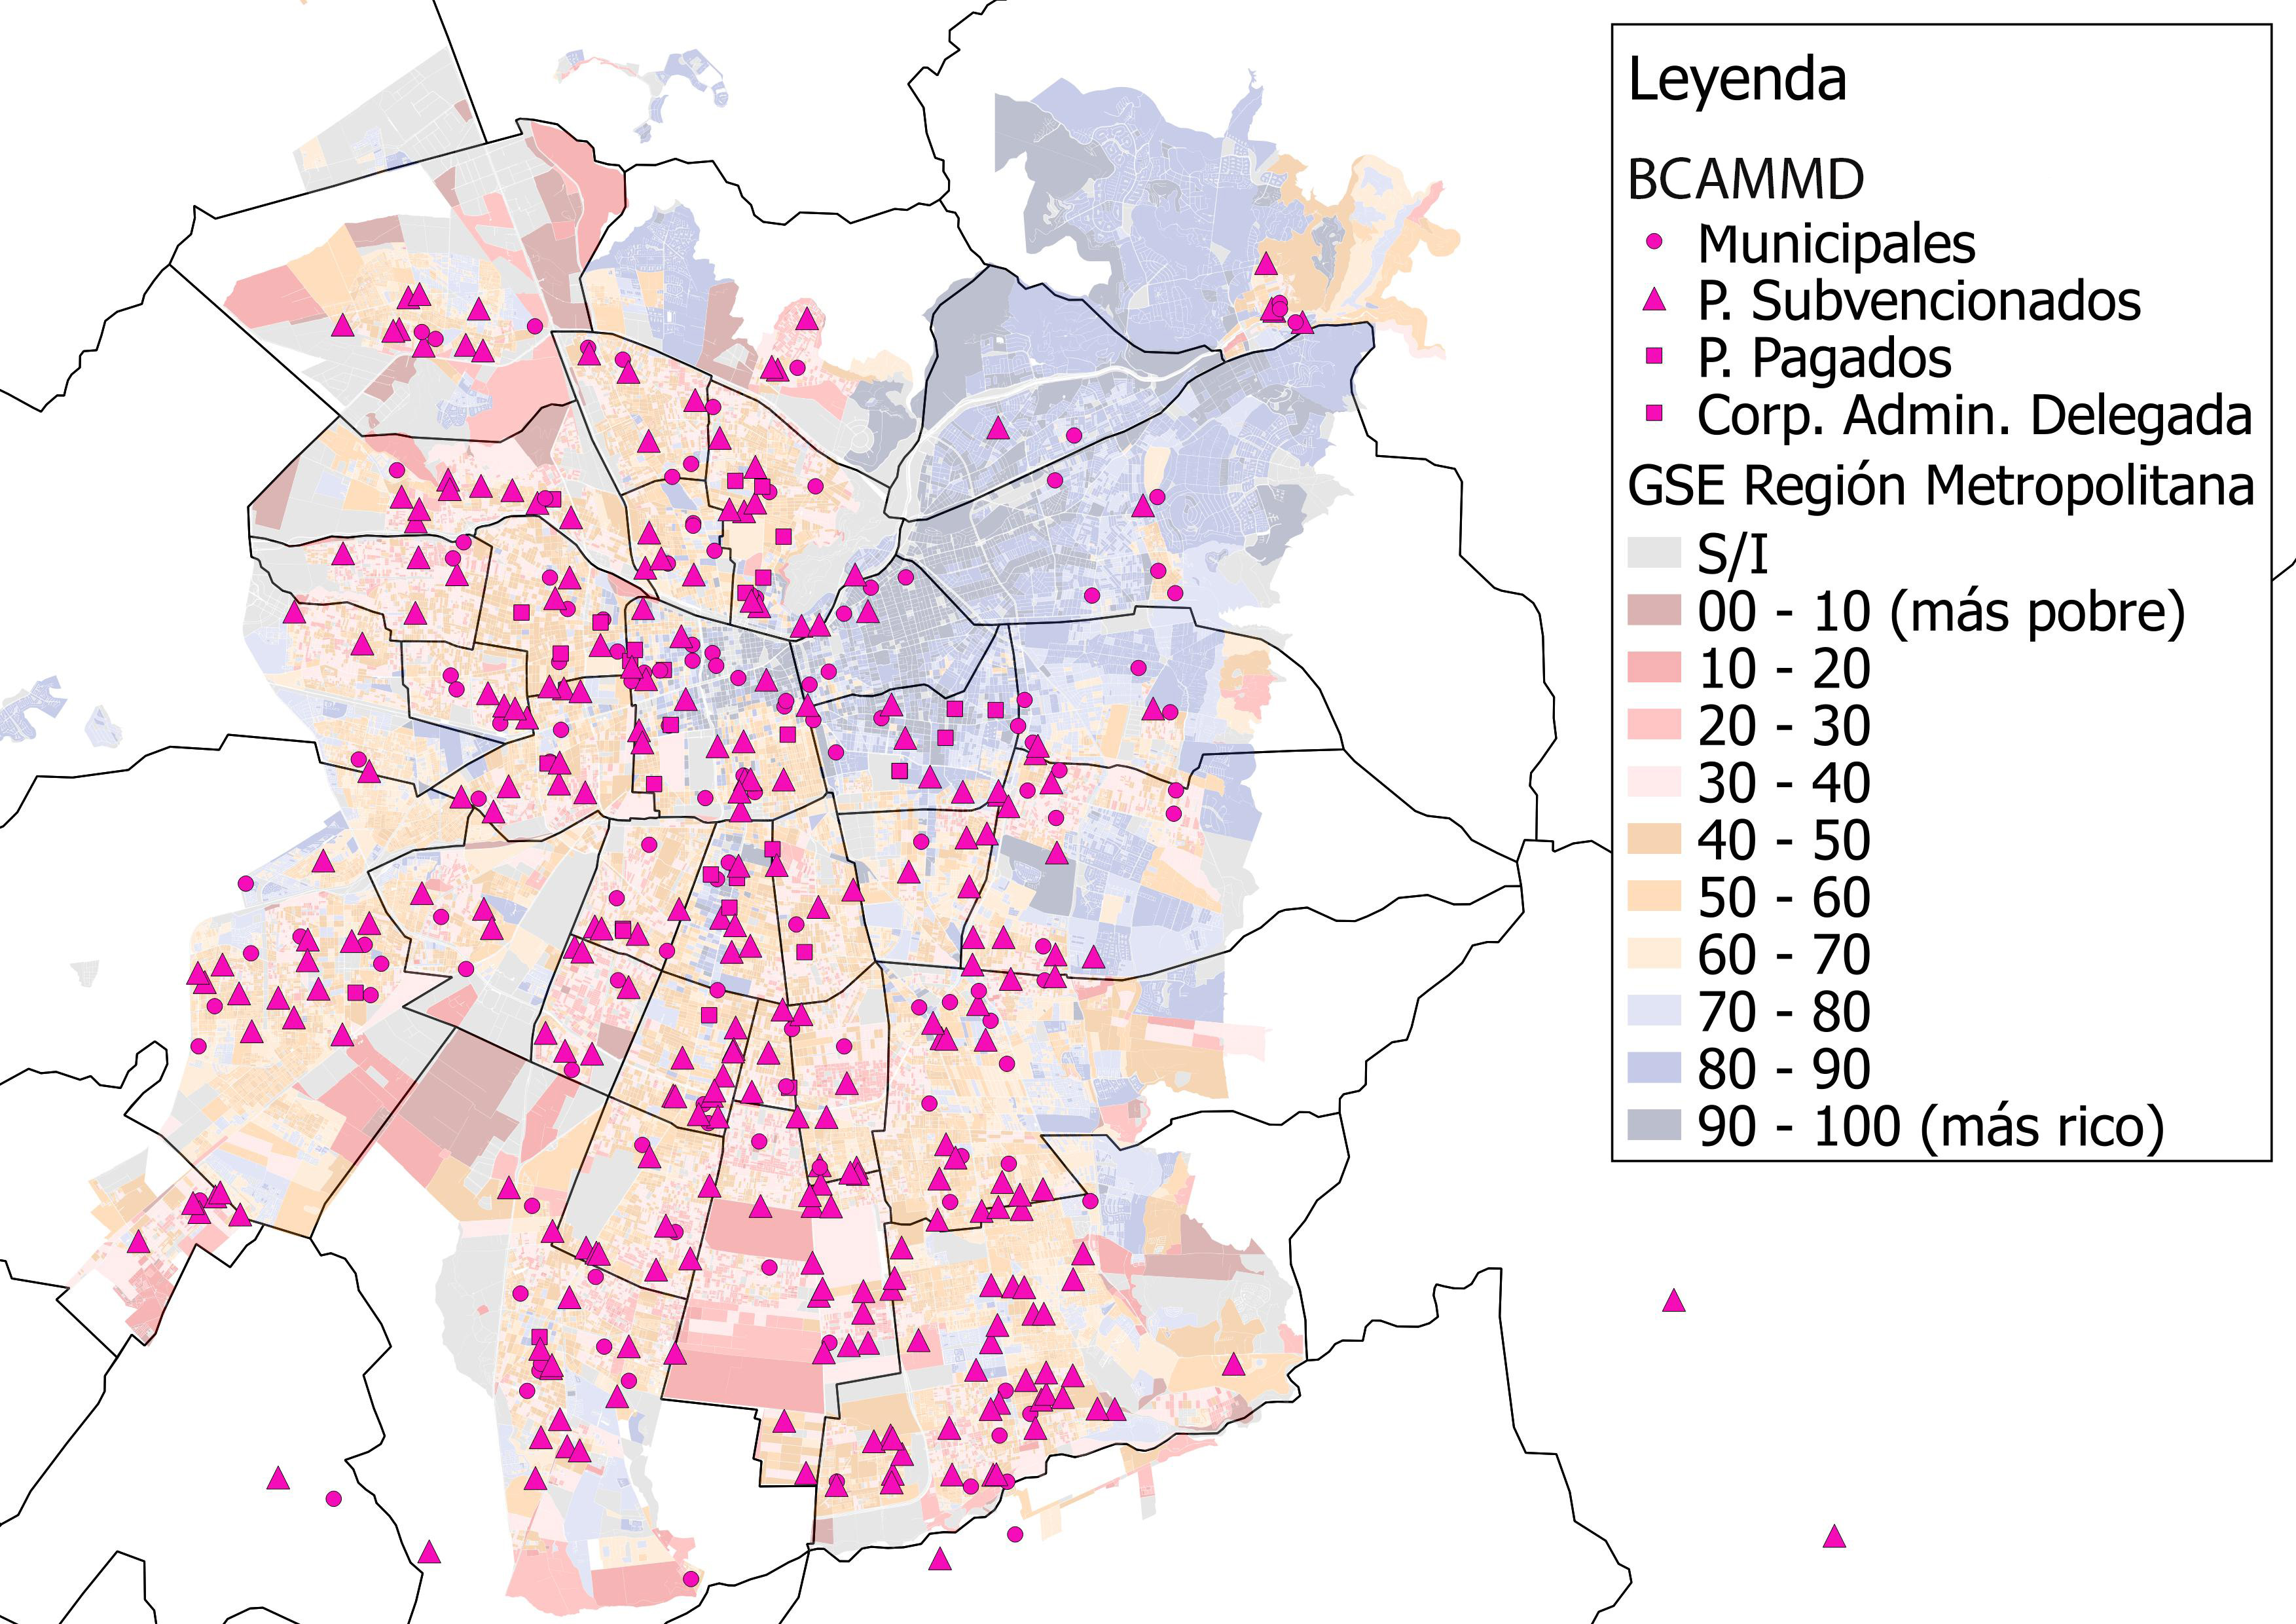
\includegraphics[width=7.5cm]{images/establecimientos/E_TODOS_CON_1.jpg}}\hspace{1mm}
  \subfloat[Establecimientos clúster E\_TODOS\_CON\_2.]{
   \label{f:mapa_estab_con_0}
    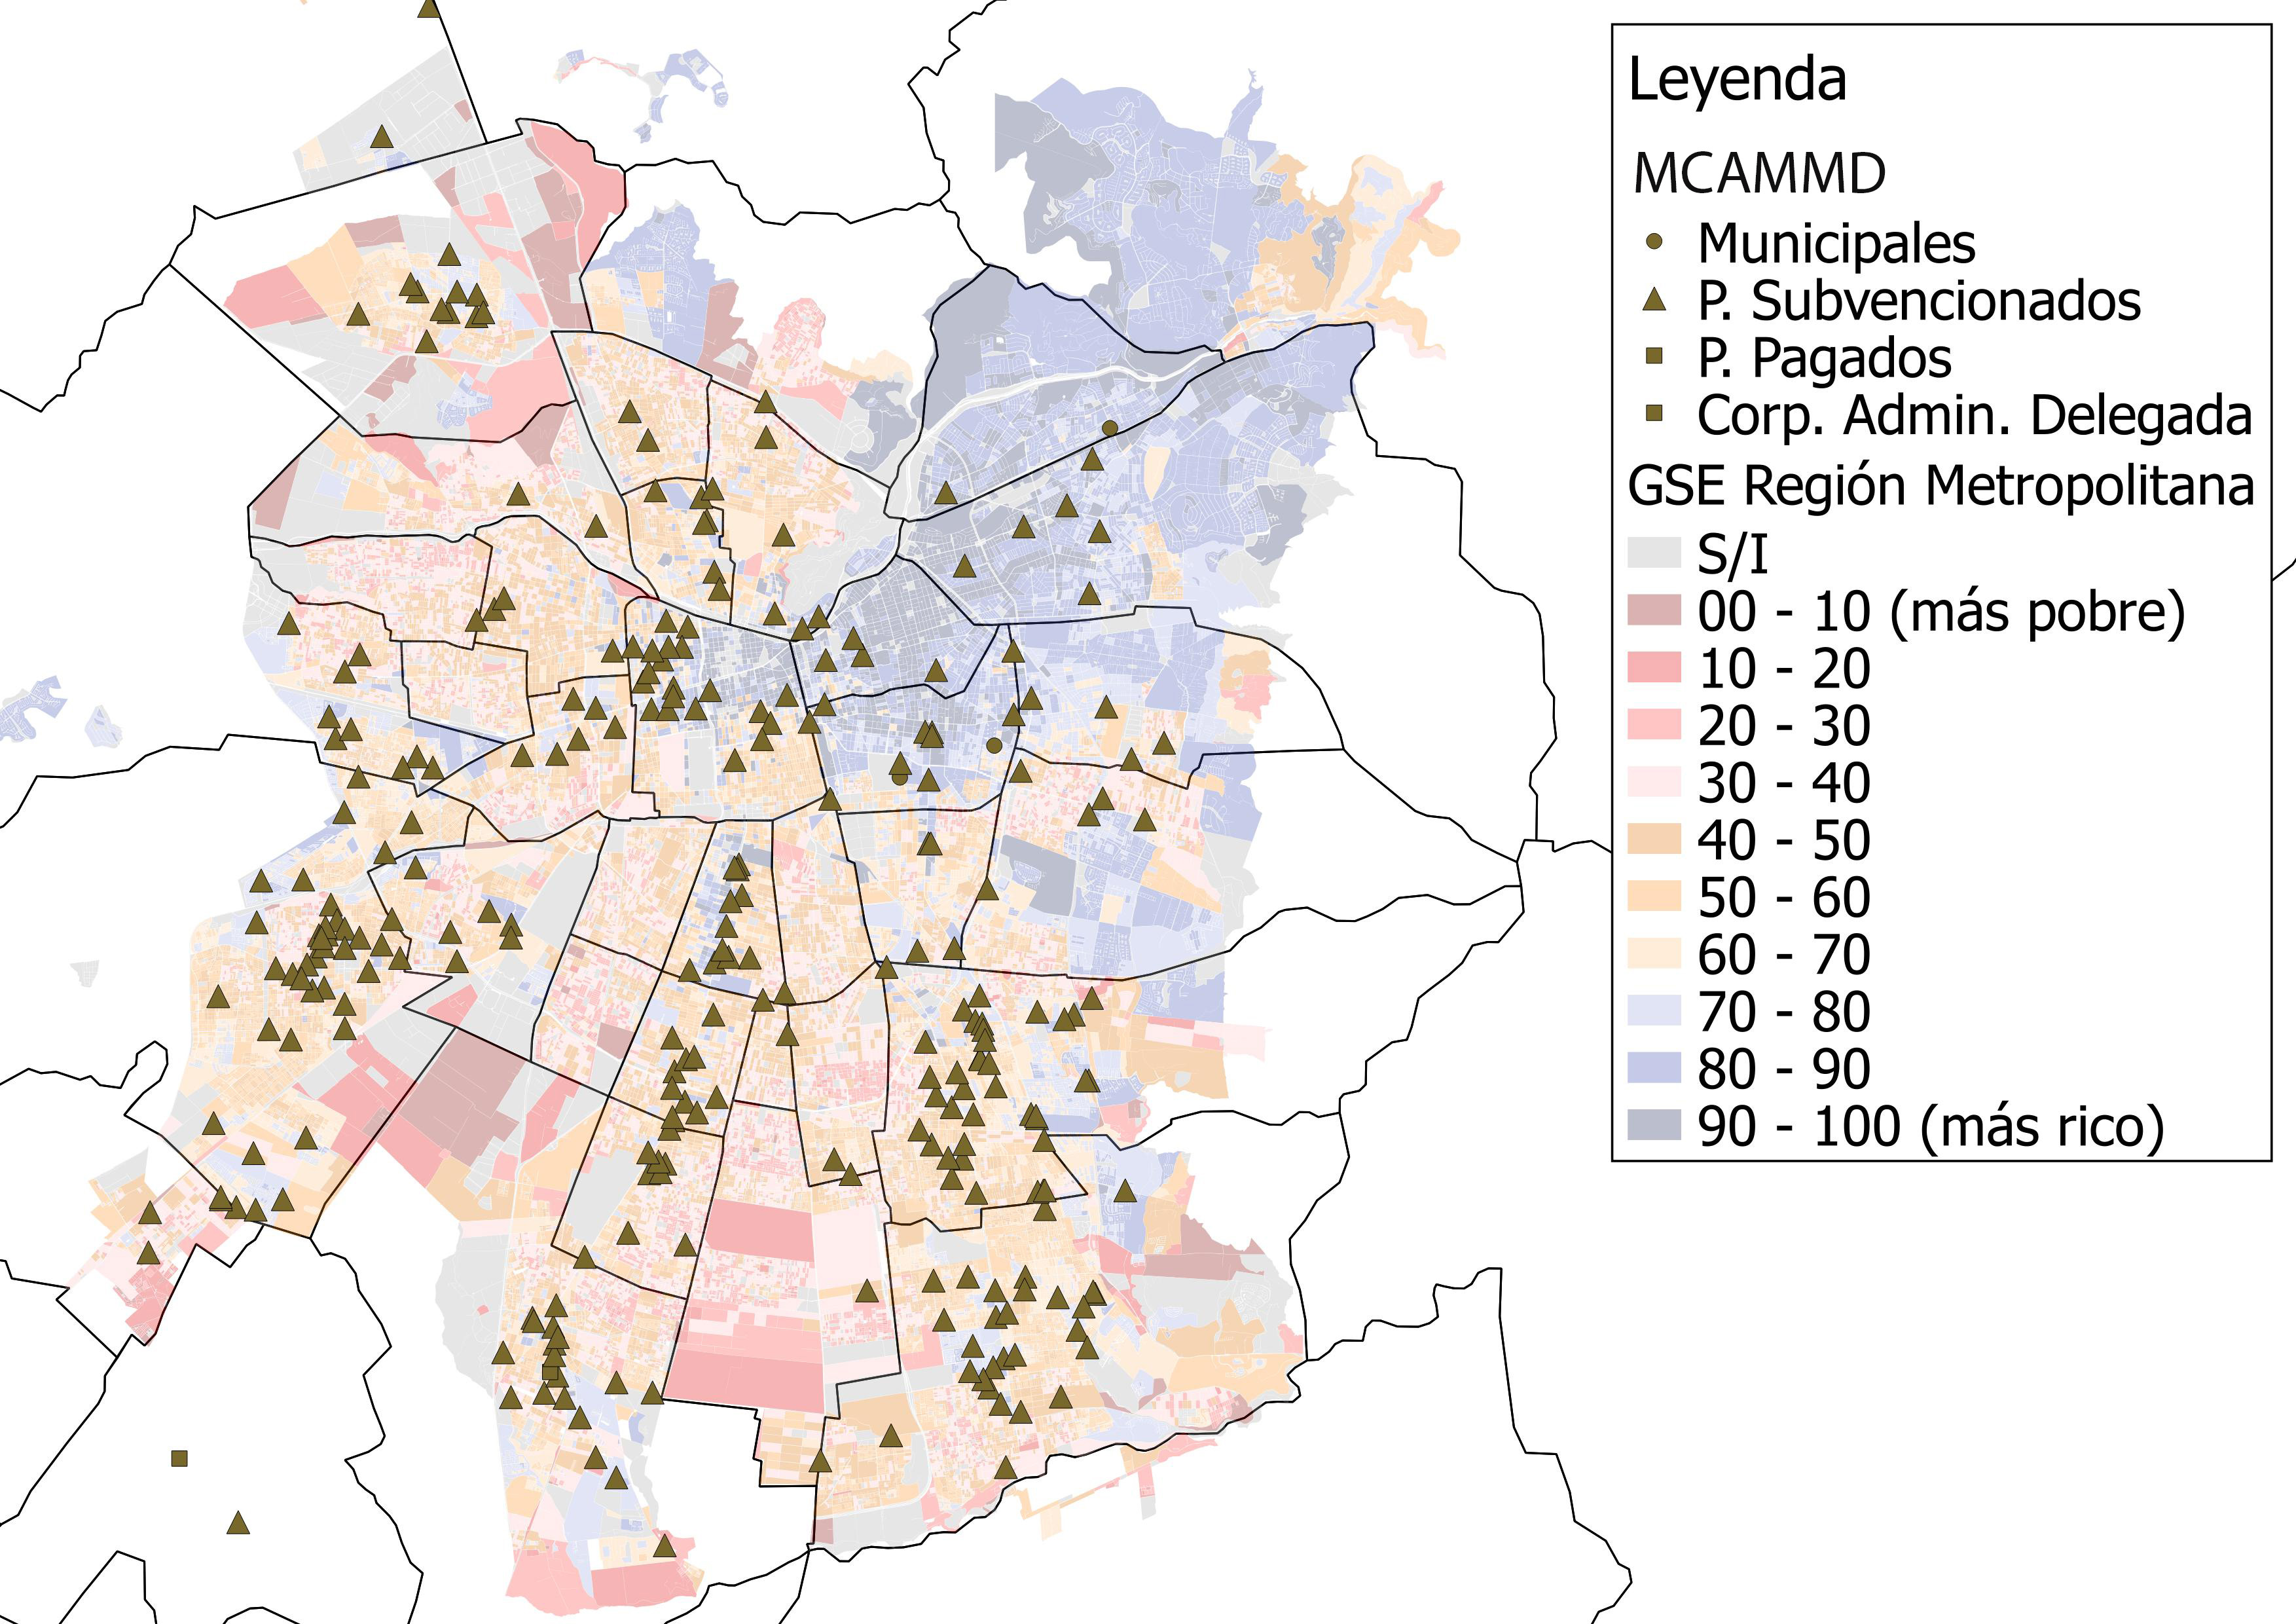
\includegraphics[width=7.5cm]{images/establecimientos/E_TODOS_CON_2.jpg}}
  \subfloat[Establecimientos clúster E\_TODOS\_CON\_3.]{
   \label{f:mapa_estab_con_0}
    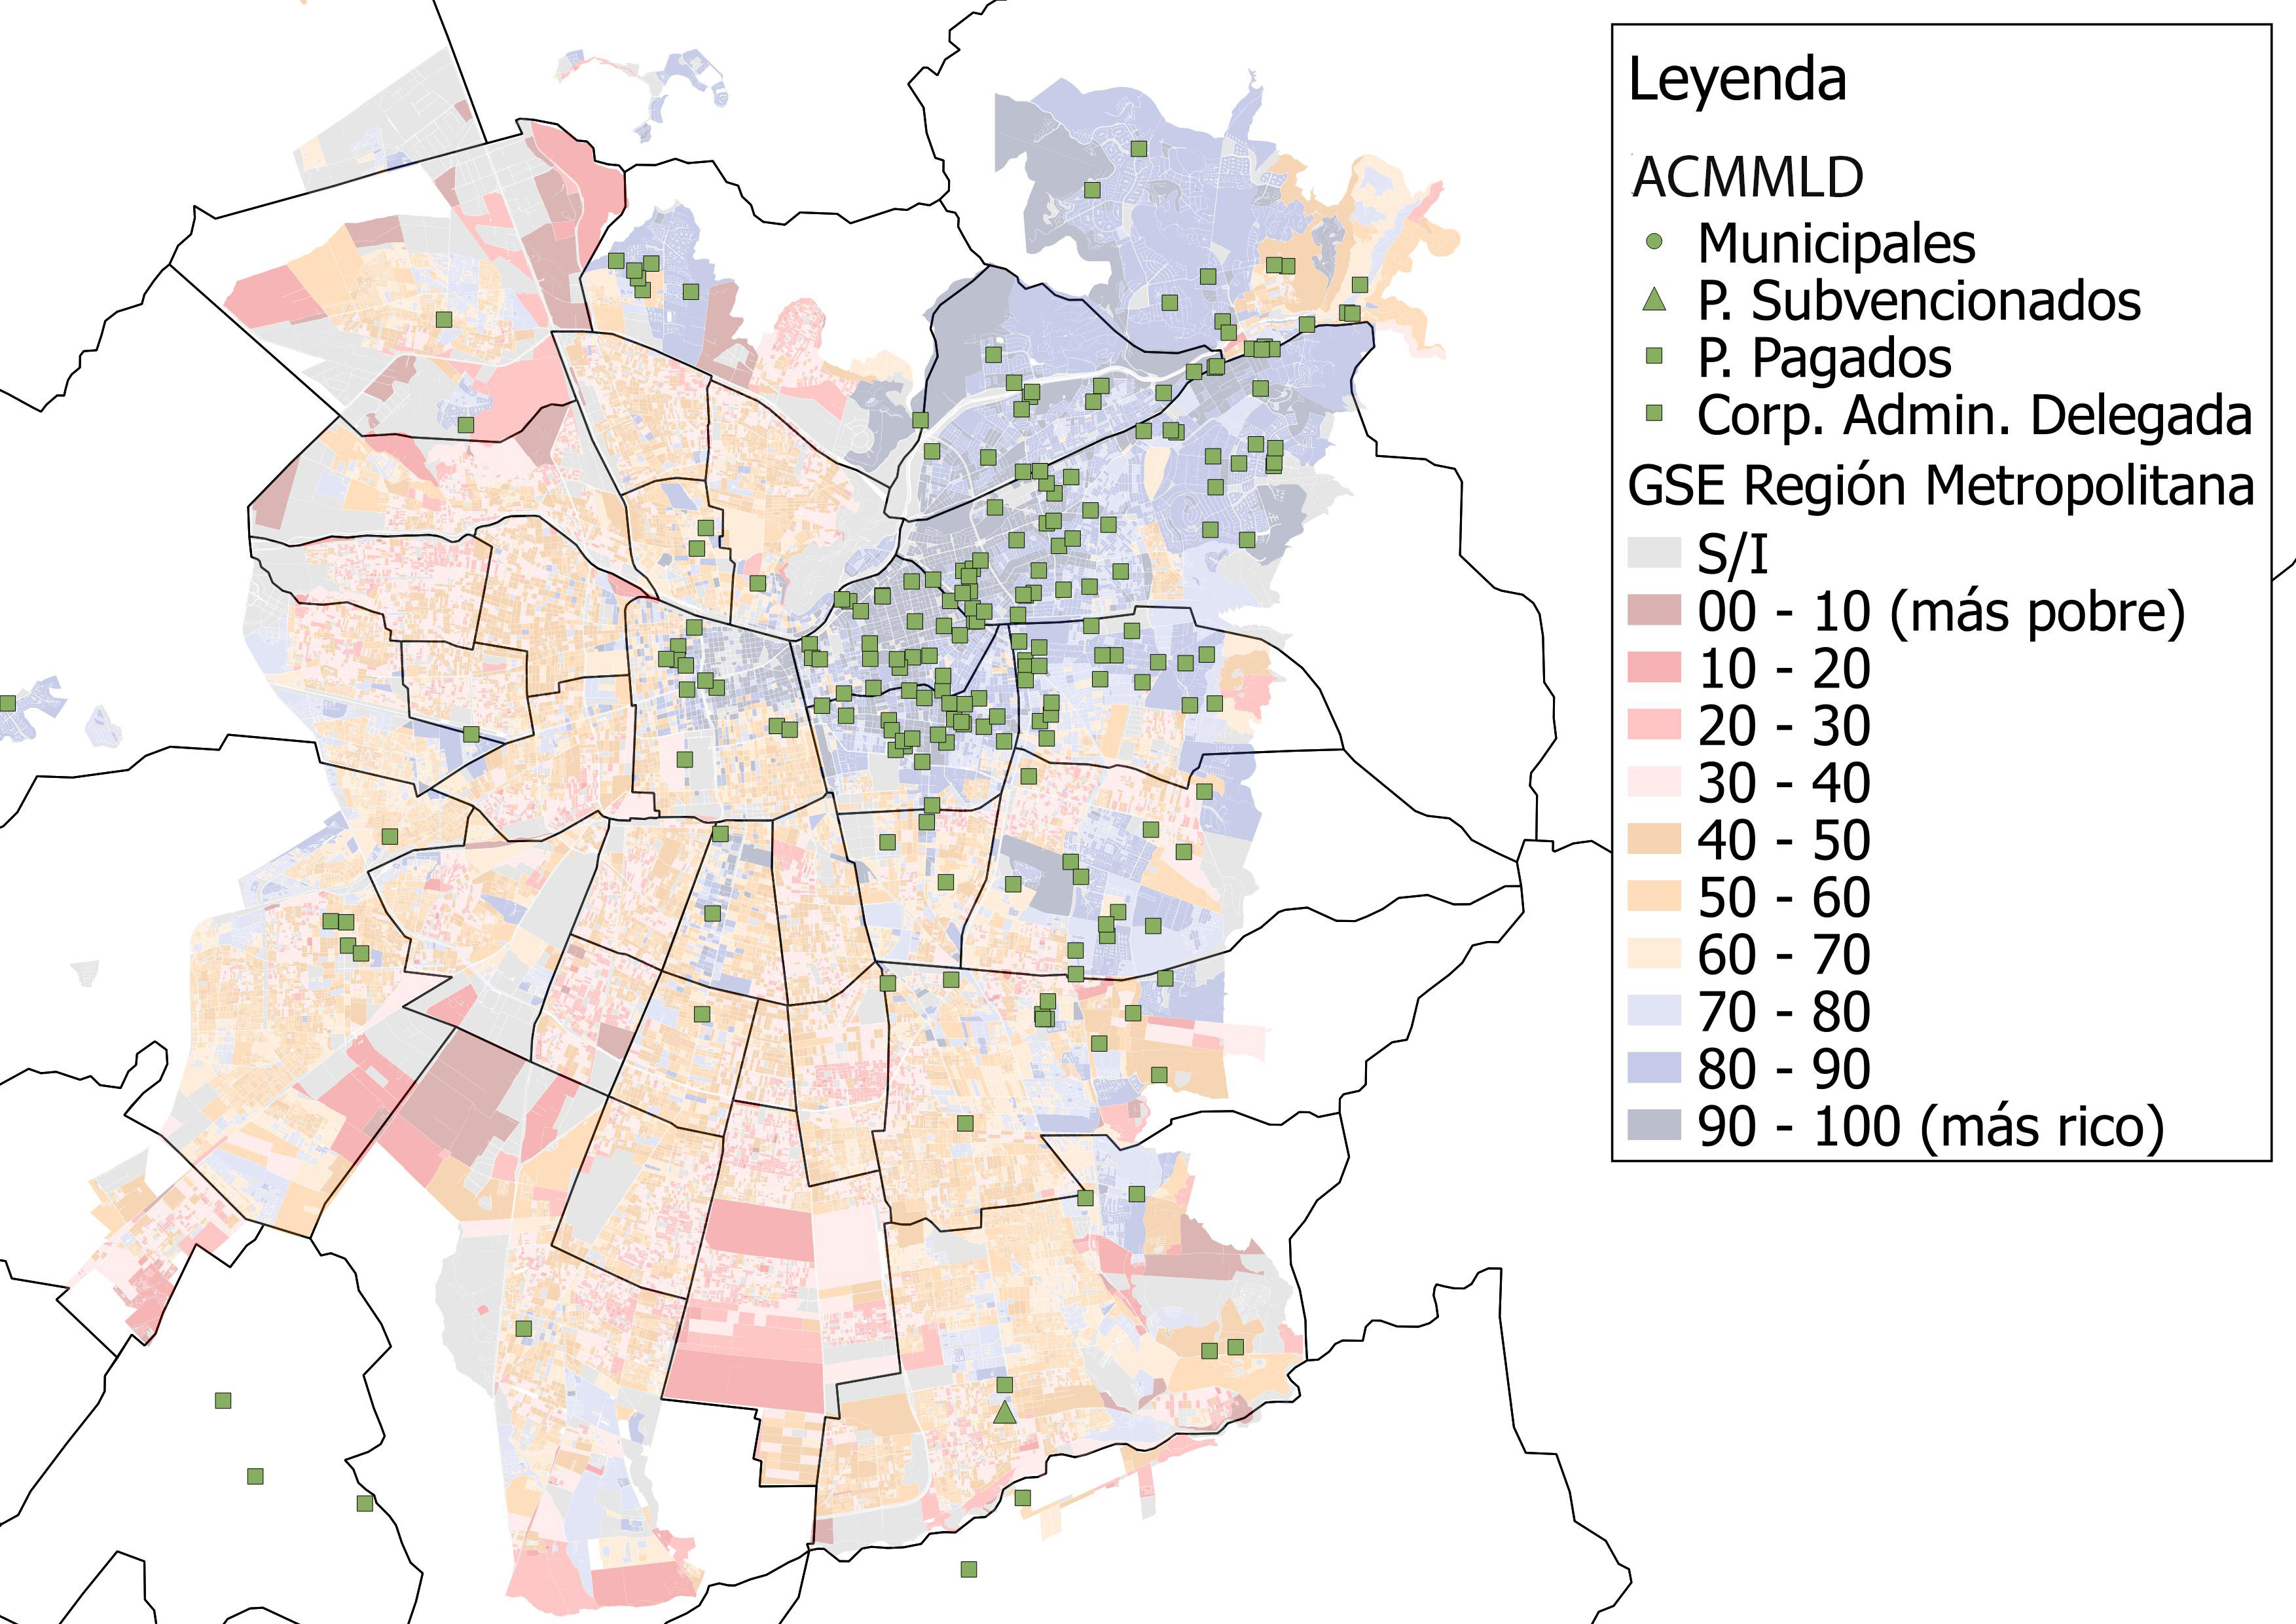
\includegraphics[width=7.5cm]{images/establecimientos/E_TODOS_CON_3.jpg}}
 \caption{Mapas de clústers de establecimientos (con atributos relacionales) sobre mapa GSE de la Región Metropolitana.}
 \label{f:mapas_estab_con_gse}
\end{figure}

En las siguientes figuras (\ref{f:mapas_mat_en_estab_sin_gse} y \ref{f:mapas_mat_en_estab_con_gse}) se muestra la distribución de los alumnos que asisten a los establecimientos de los diferentes clústers con diferentes mapas de calor. En los establecimientos del clúster E\_TODOS\_SIN\_0 los alumnos se distribuyen por casi toda el área metropolitana, pero se concentran principalmente en un sector de la zona sur y poniente. En la siguiente (\ref{f:mapa_mat_en_estab_sin_1_gse}), la que representa las matrículas del clúster E\_TODOS\_SIN\_0, los alumnos se distribuyen por toda el área, pero en menor proporción y densidad en el sector oriente. En \ref{f:mapa_estab_sin_2} la distribución del alumnado se da por toda el área metropolitana, aunque se encuentra de manera mas densa en la periferia del sector poniente, seguida por dos sectores del sur de la capital. Por último, en el cuarto clúster todos sus estudiantes se sitúan en el sector oriente, concentrándose en el sector más periférico de esta zona. 

En los primeros tres clústers los alumnos que asisten a estos establecimientos viven en su gran mayoría en zonas pertenecientes a los deciles del 4 al 7, a diferencia del último caso en que sus estudiantes viven predominantemente en los sectores de deciles 8 al 10, es decir, es los lugares más acomodados del área metropolitana.

\begin{figure}[H]
 \centering
  \subfloat[Matrículas en colegios de E\_TODOS\_SIN\_0.]{
   \label{f:mapa_mat_en_estab_sin_0_gse}
    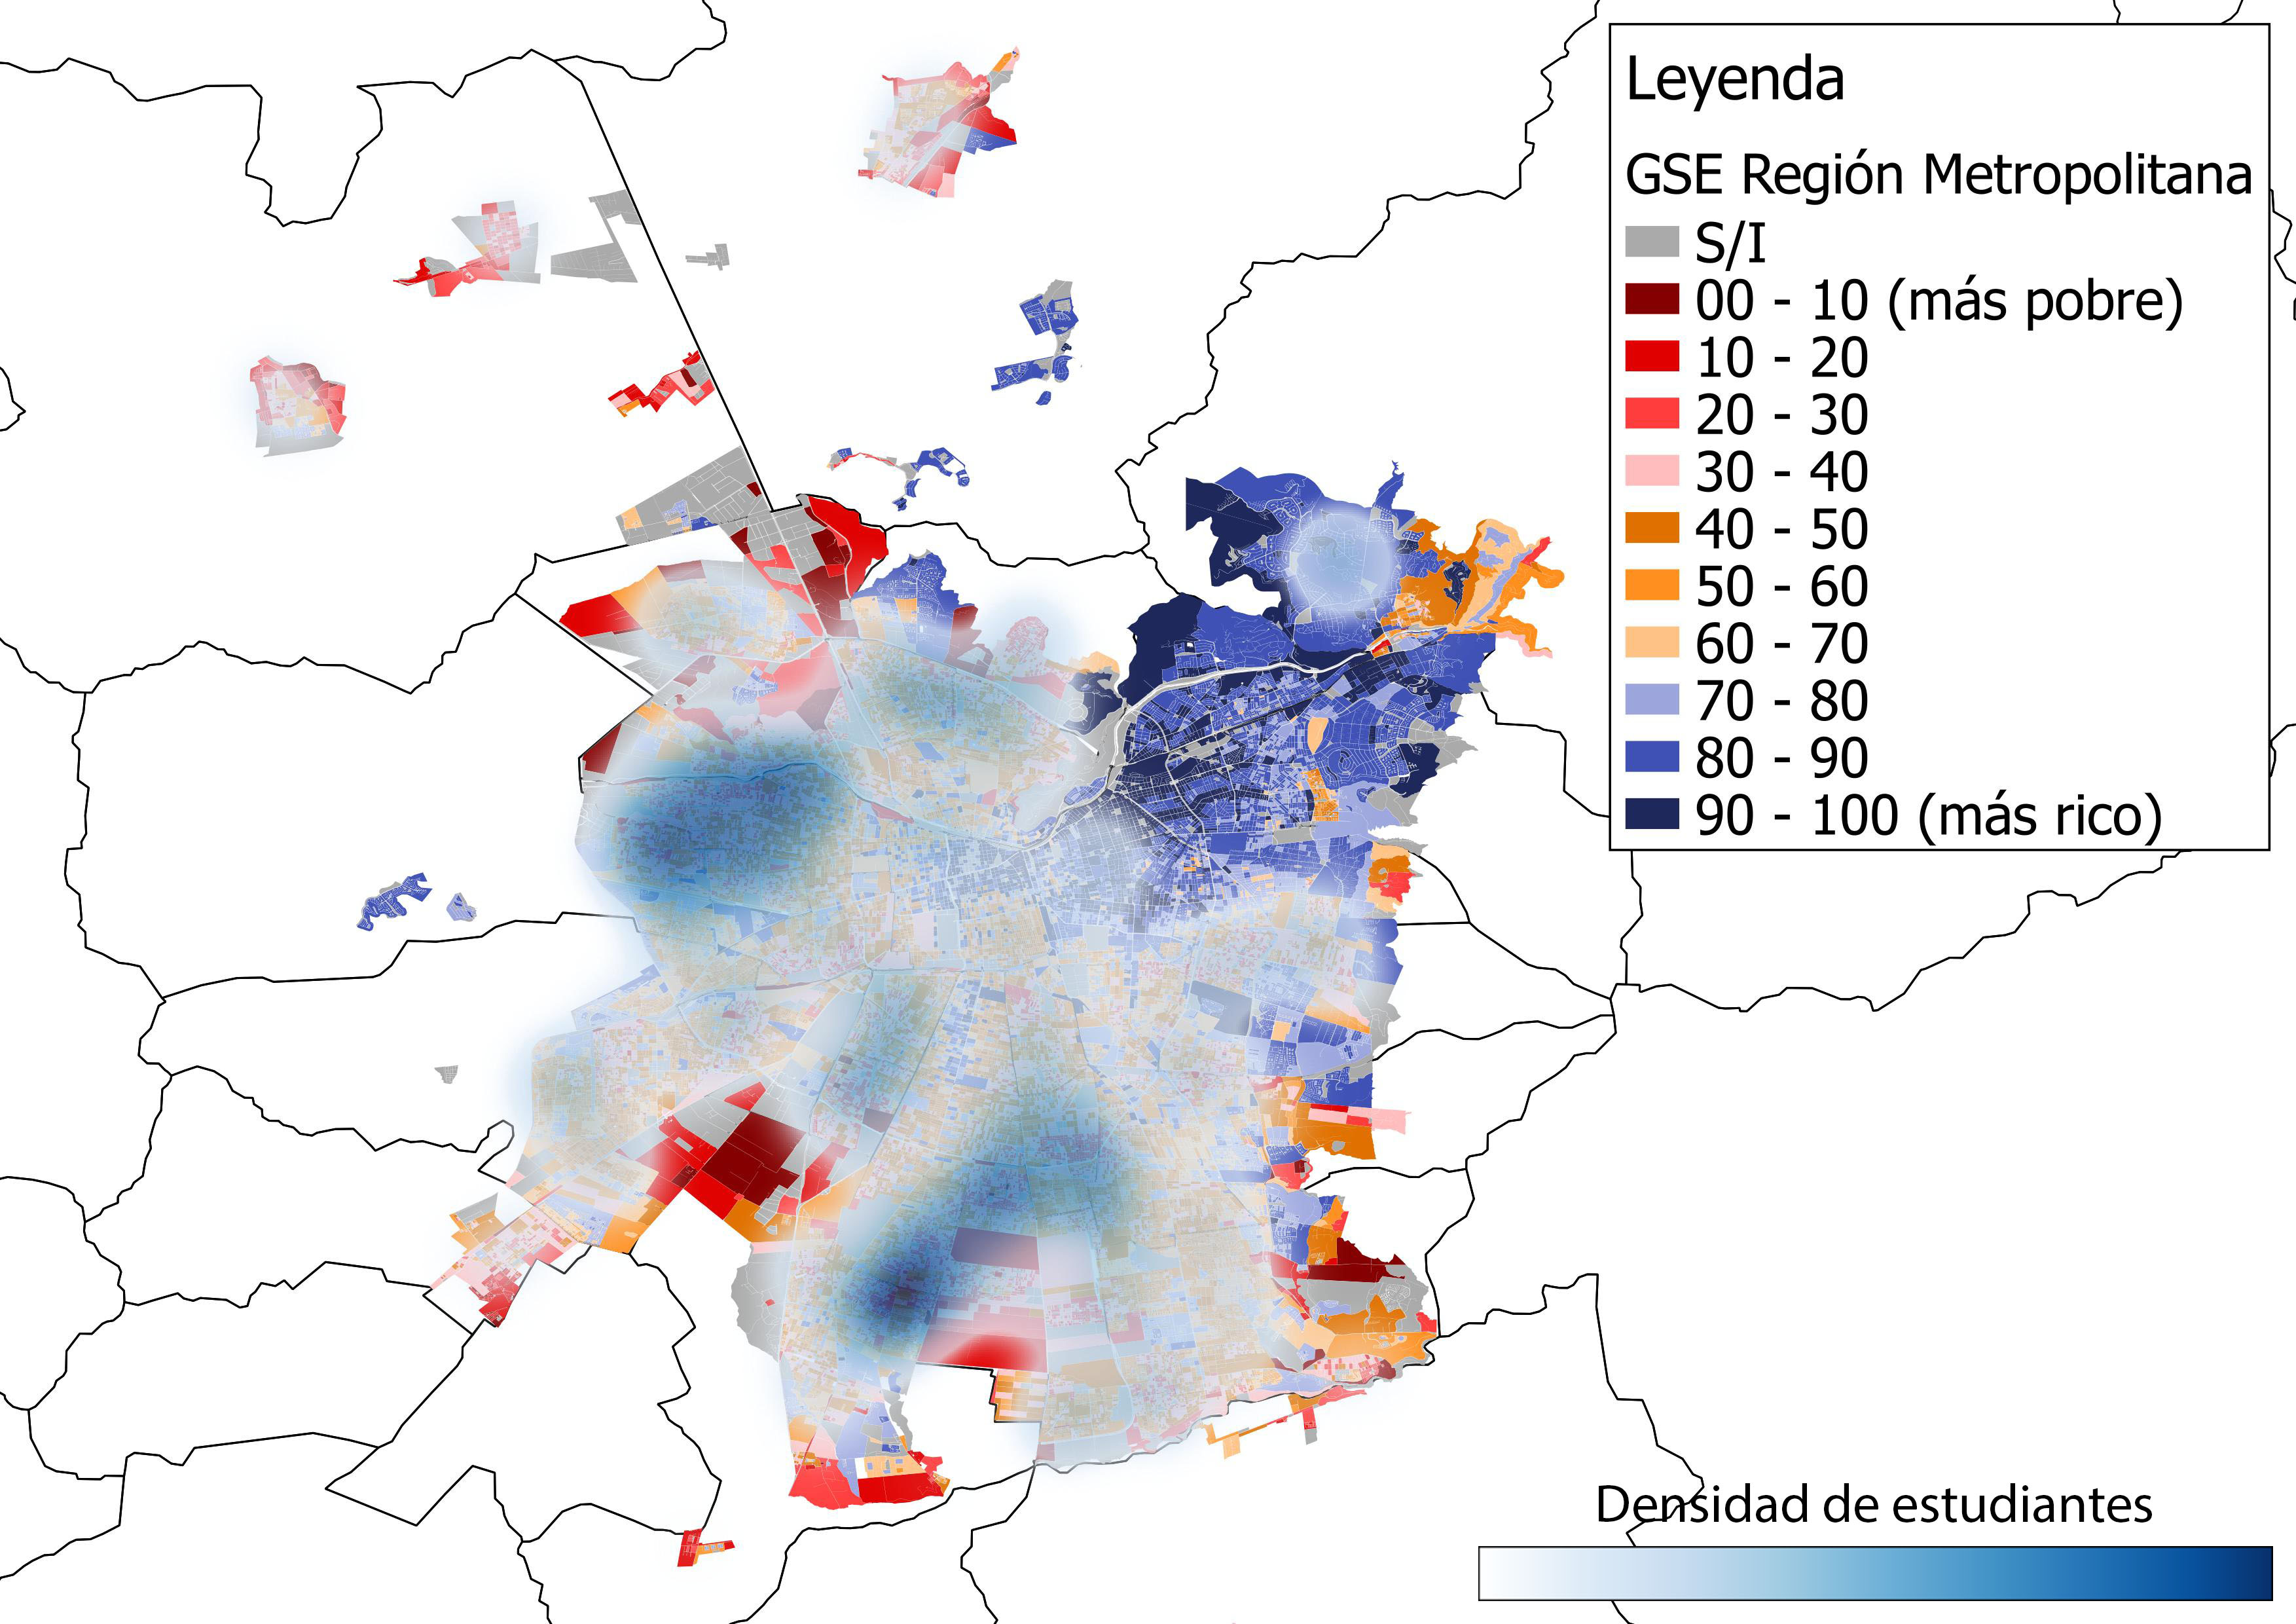
\includegraphics[width=7.5cm]{images/matriculas/E_SIN_0_final.jpg}}
  \subfloat[Matrículas en colegios de E\_TODOS\_SIN\_1.]{
   \label{f:mapa_mat_en_estab_sin_1_gse}
    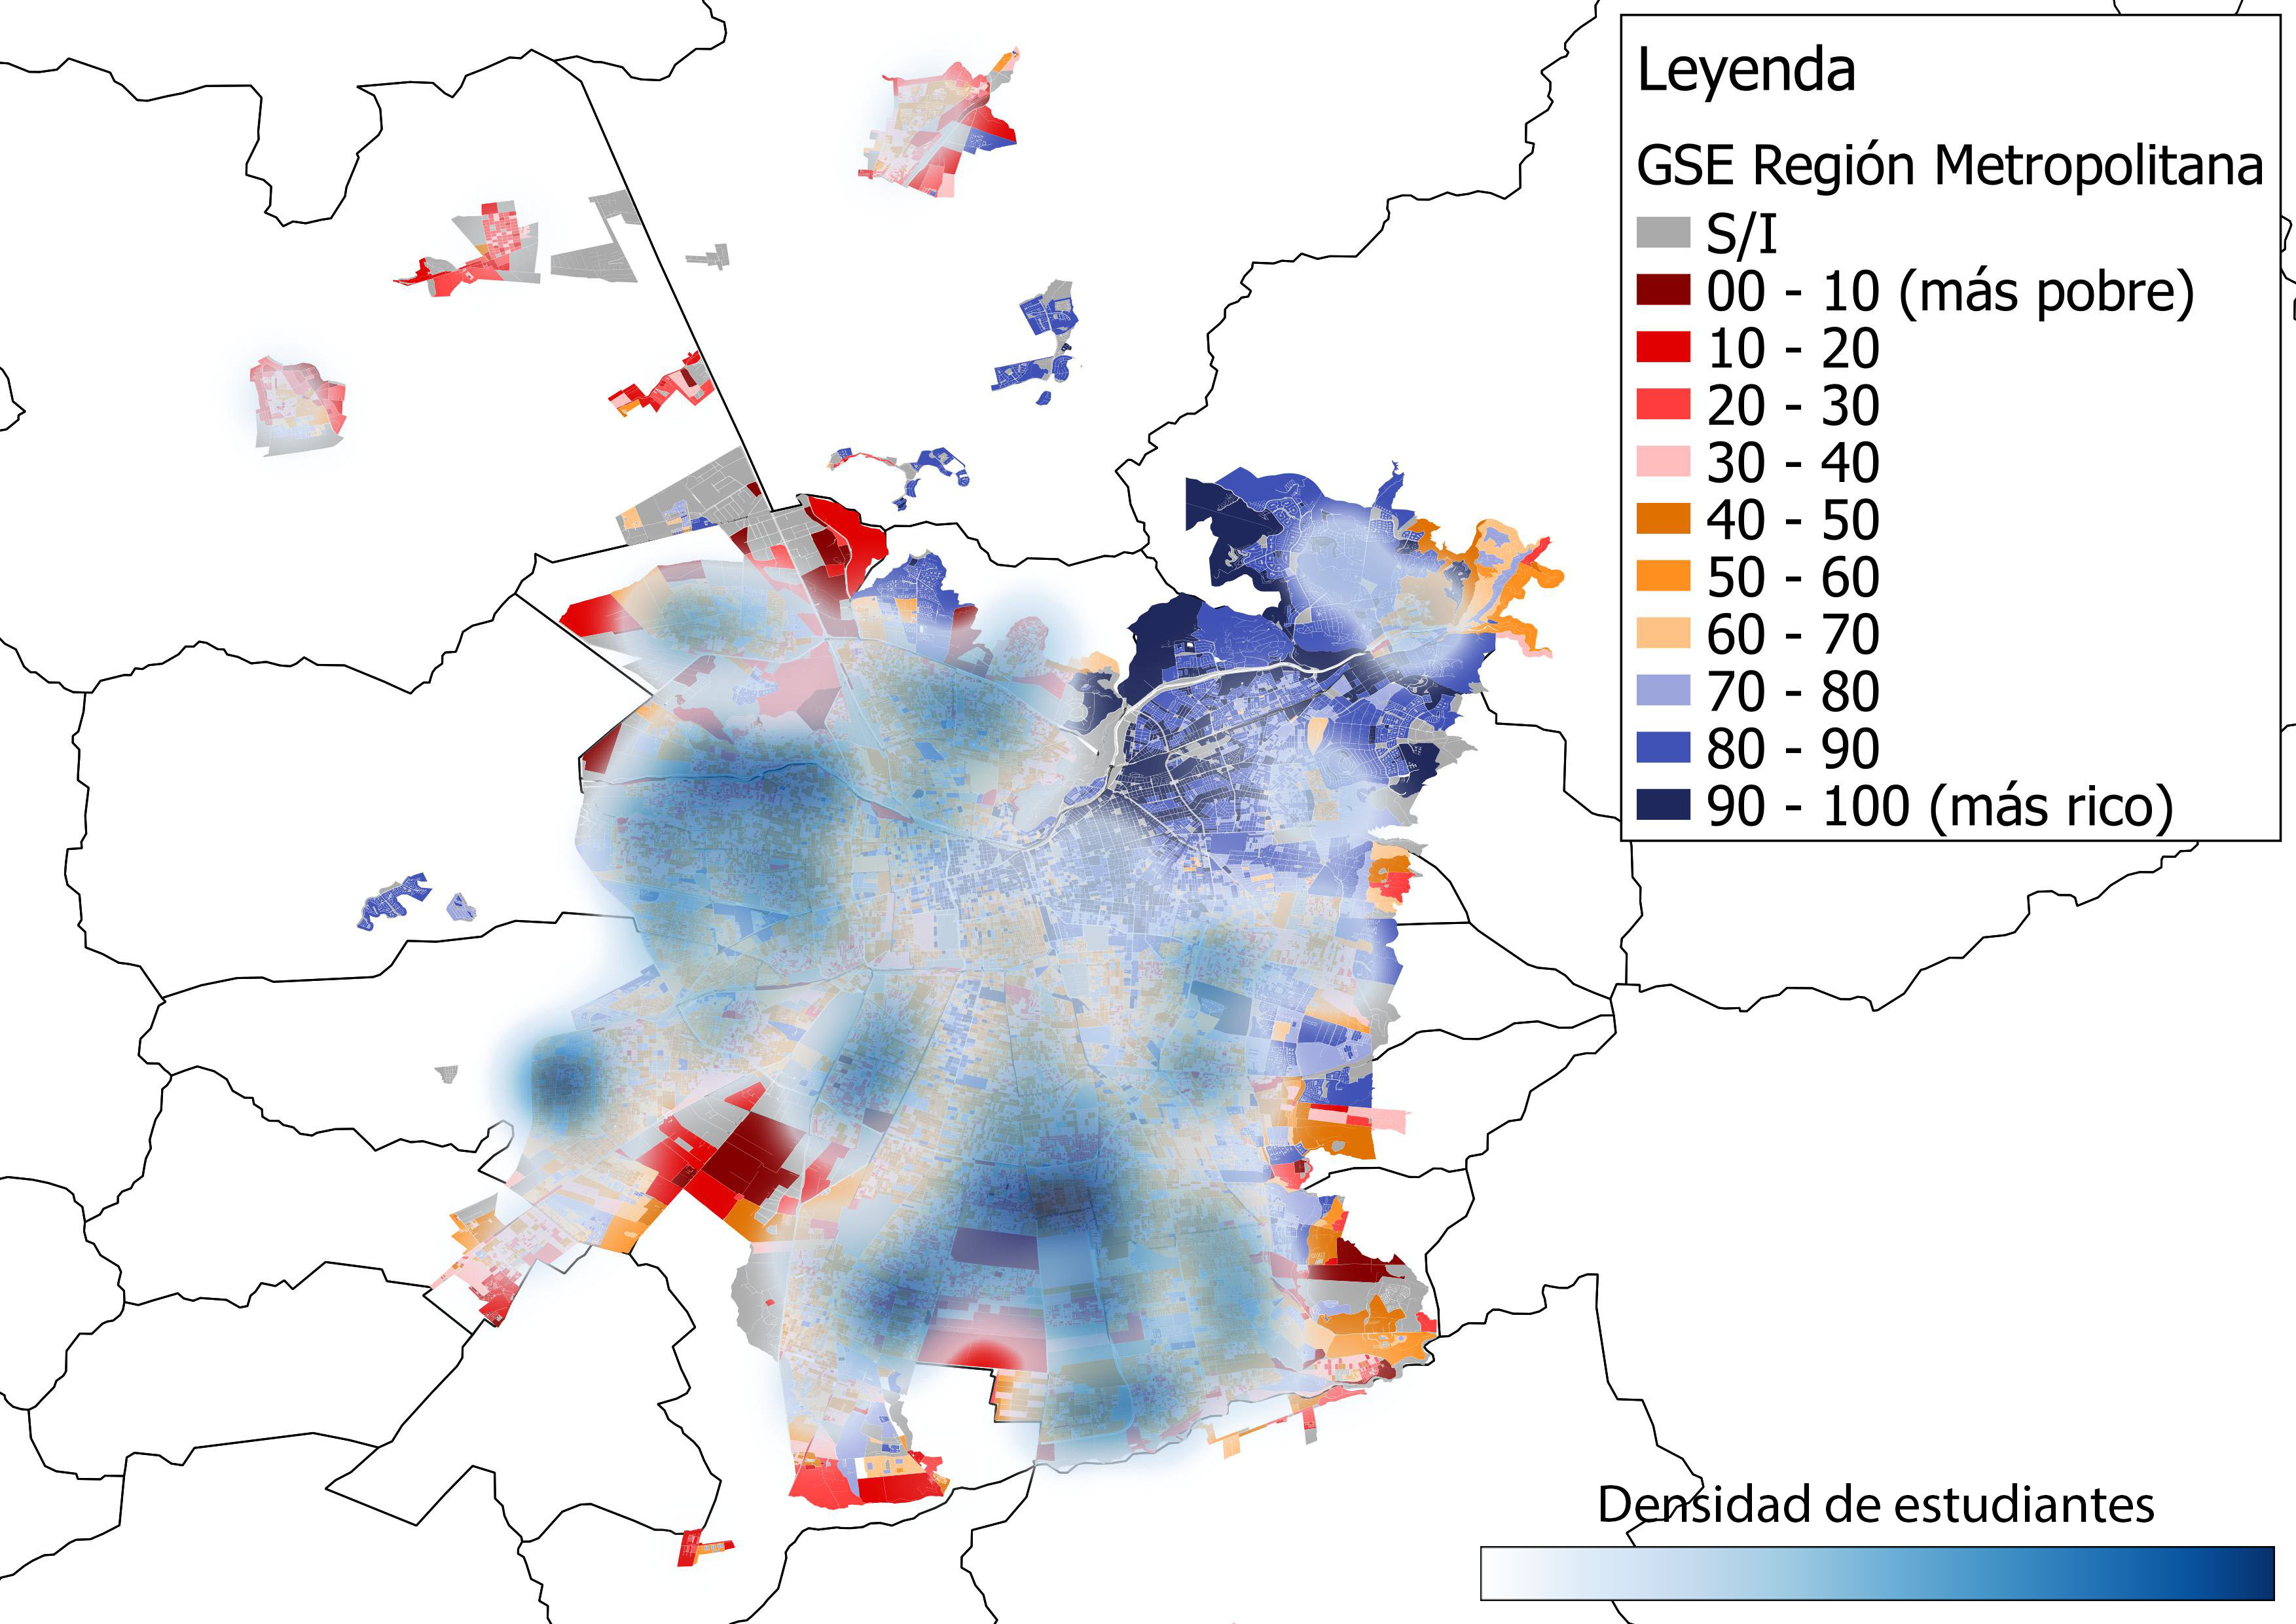
\includegraphics[width=7.5cm]{images/matriculas/E_SIN_1_final.jpg}}\hspace{1mm}
  \subfloat[Matrículas en colegios de E\_TODOS\_SIN\_2.]{
   \label{f:mapa_mat_en_estab_sin_2_gse}
    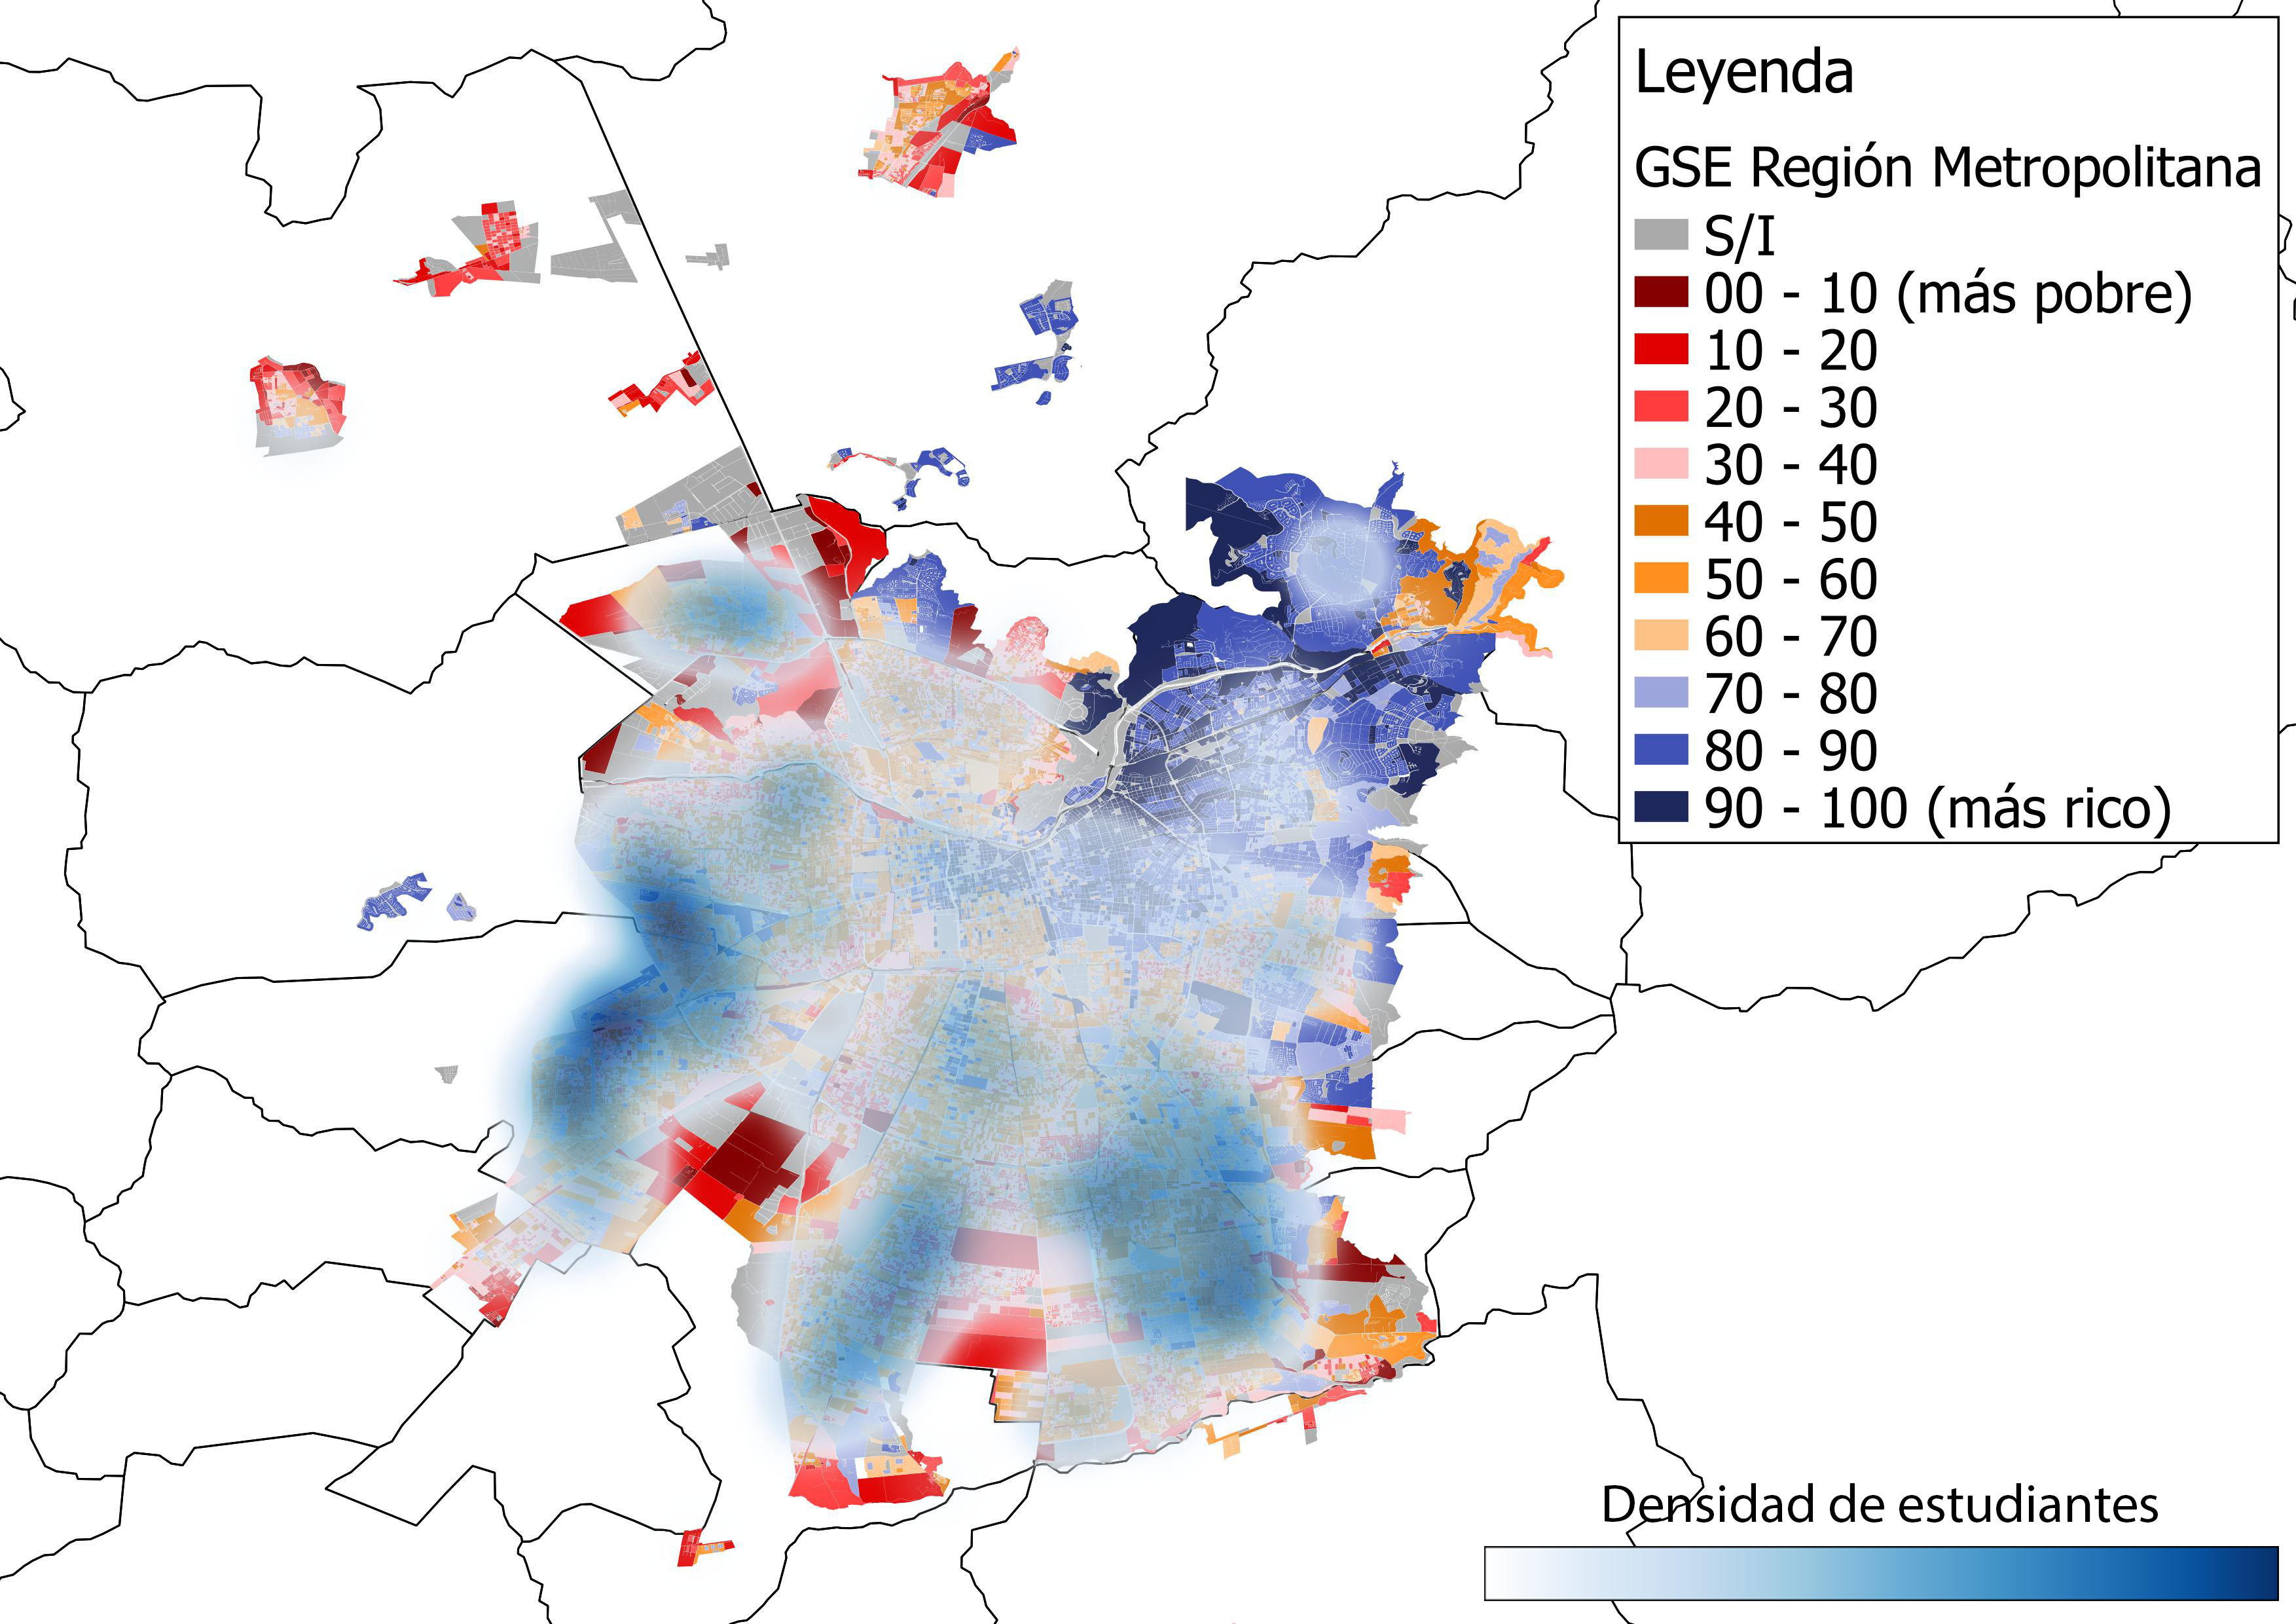
\includegraphics[width=7.5cm]{images/matriculas/E_SIN_2_final.jpg}}
  \subfloat[Matrículas en colegios de E\_TODOS\_SIN\_3.]{
   \label{f:mapa_mat_en_estab_sin_3_gse}
    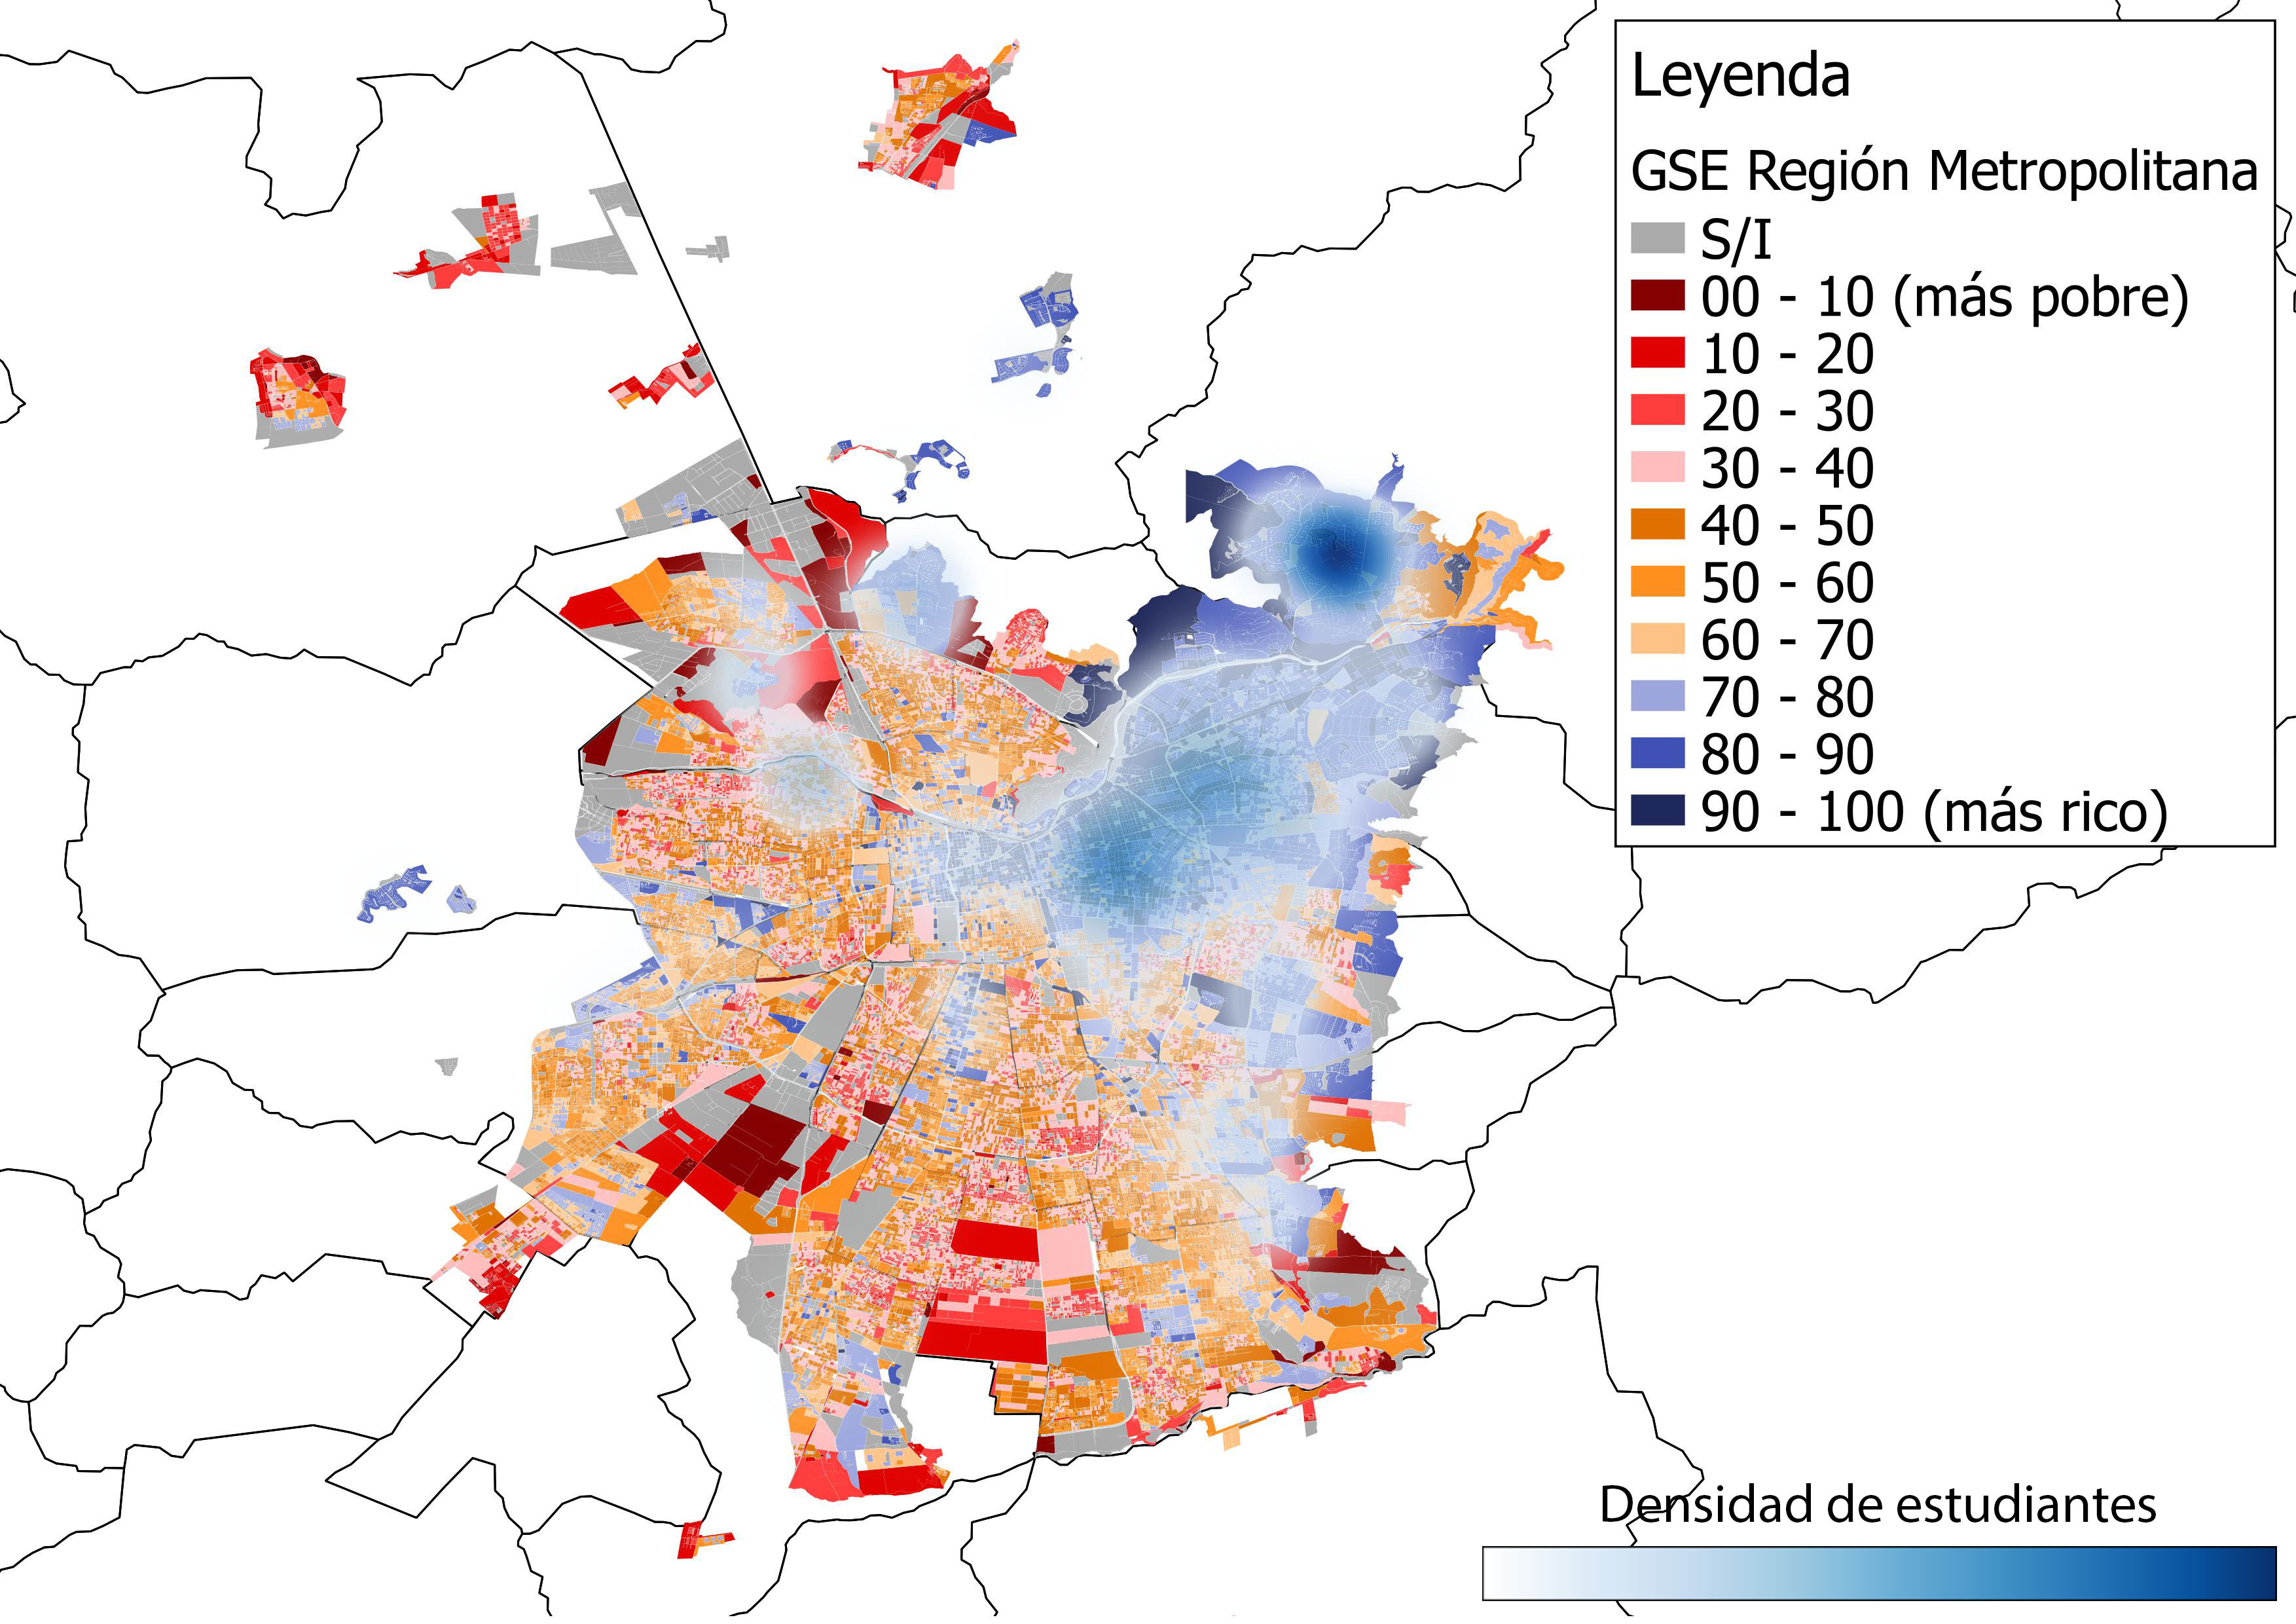
\includegraphics[width=7.5cm]{images/matriculas/E_SIN_3_final.jpg}}
 \caption{Mapas de calor de matrículas en clústers de establecimientos sobre mapa GSE de la Región Metropolitana.}
 \label{f:mapas_mat_en_estab_sin_gse}
\end{figure}

Como los clúster de establecimientos no presentan cambios importantes al ser analizados con y sin variables de relación establecimiento - matrícula, sus resultados son similares, por lo que las figuras \ref{f:mapas_mat_en_estab_sin_gse} y \ref{f:mapas_mat_en_estab_con_gse} son casi idénticas y es díficil percibir alguna variación entre ellas.

\begin{figure}[H]
 \centering
  \subfloat[Matrículas en colegios de E\_TODOS\_CON\_0.]{
   \label{f:mapa_mat_en_estab_con_0_gse}
    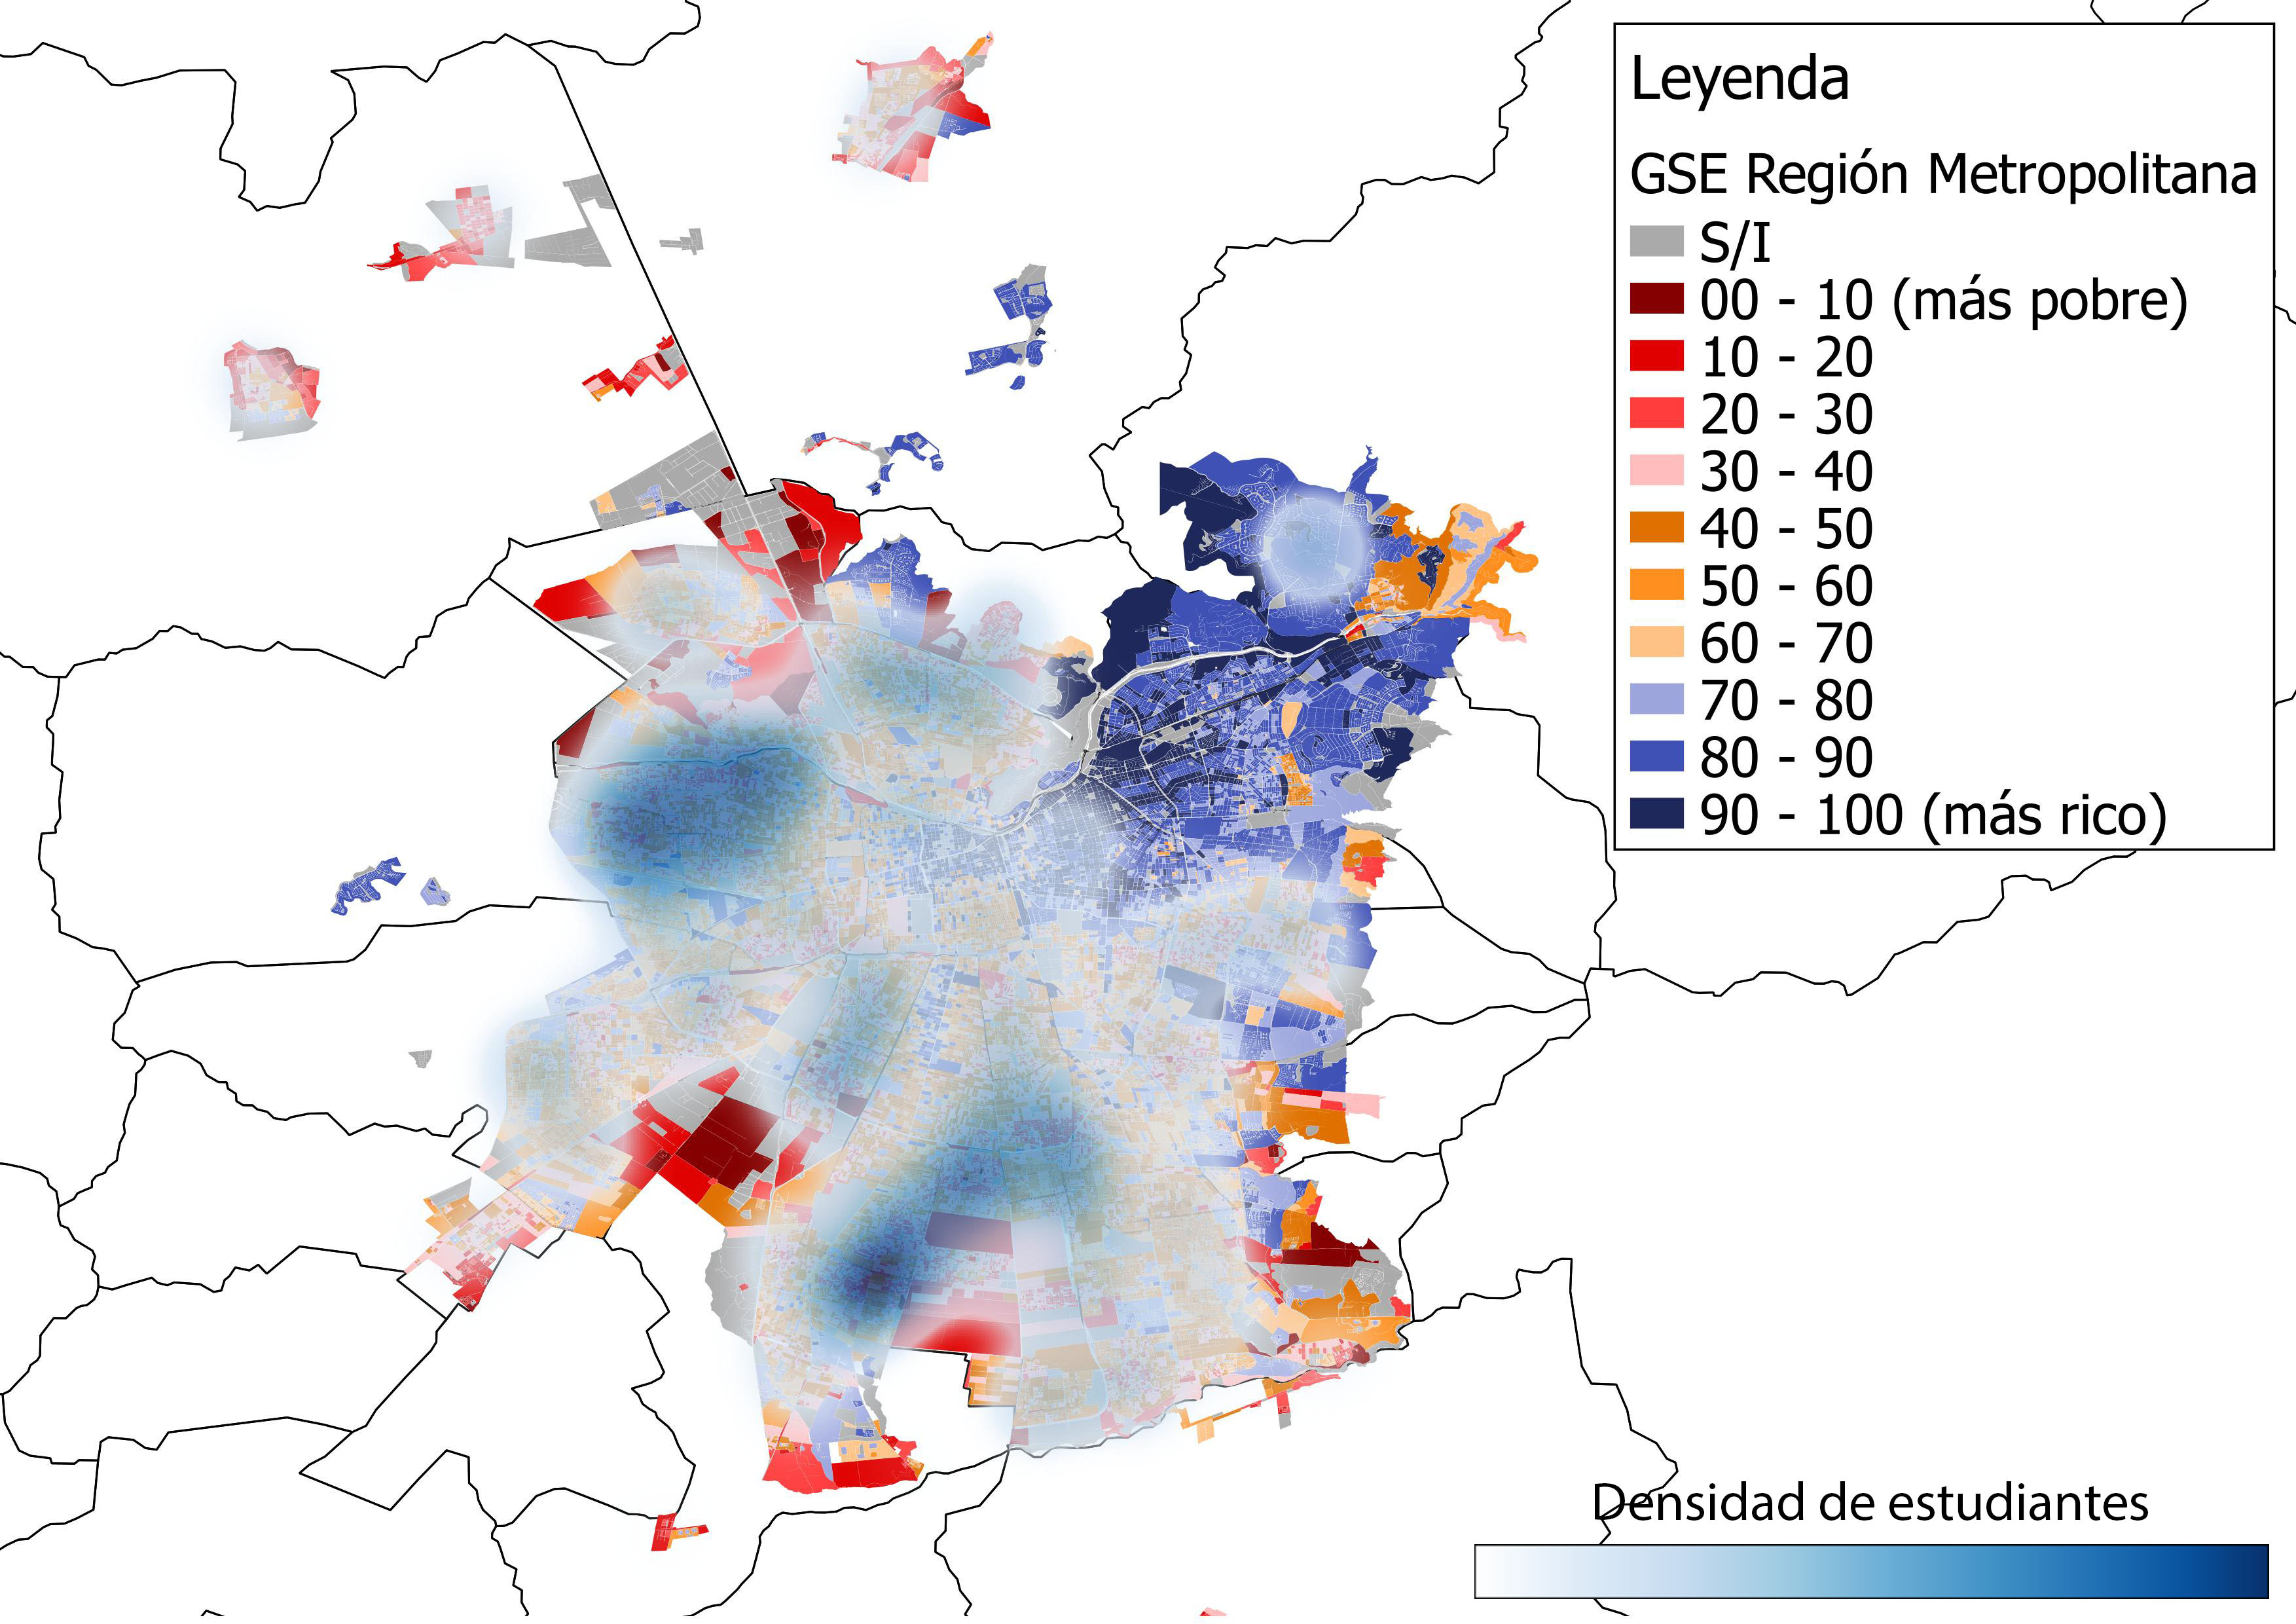
\includegraphics[width=7.5cm]{images/matriculas/E_CON_0_final.jpg}}
  \subfloat[Matrículas en colegios de E\_TODOS\_CON\_1.]{
   \label{f:mapa_mat_en_estab_con_1_gse}
    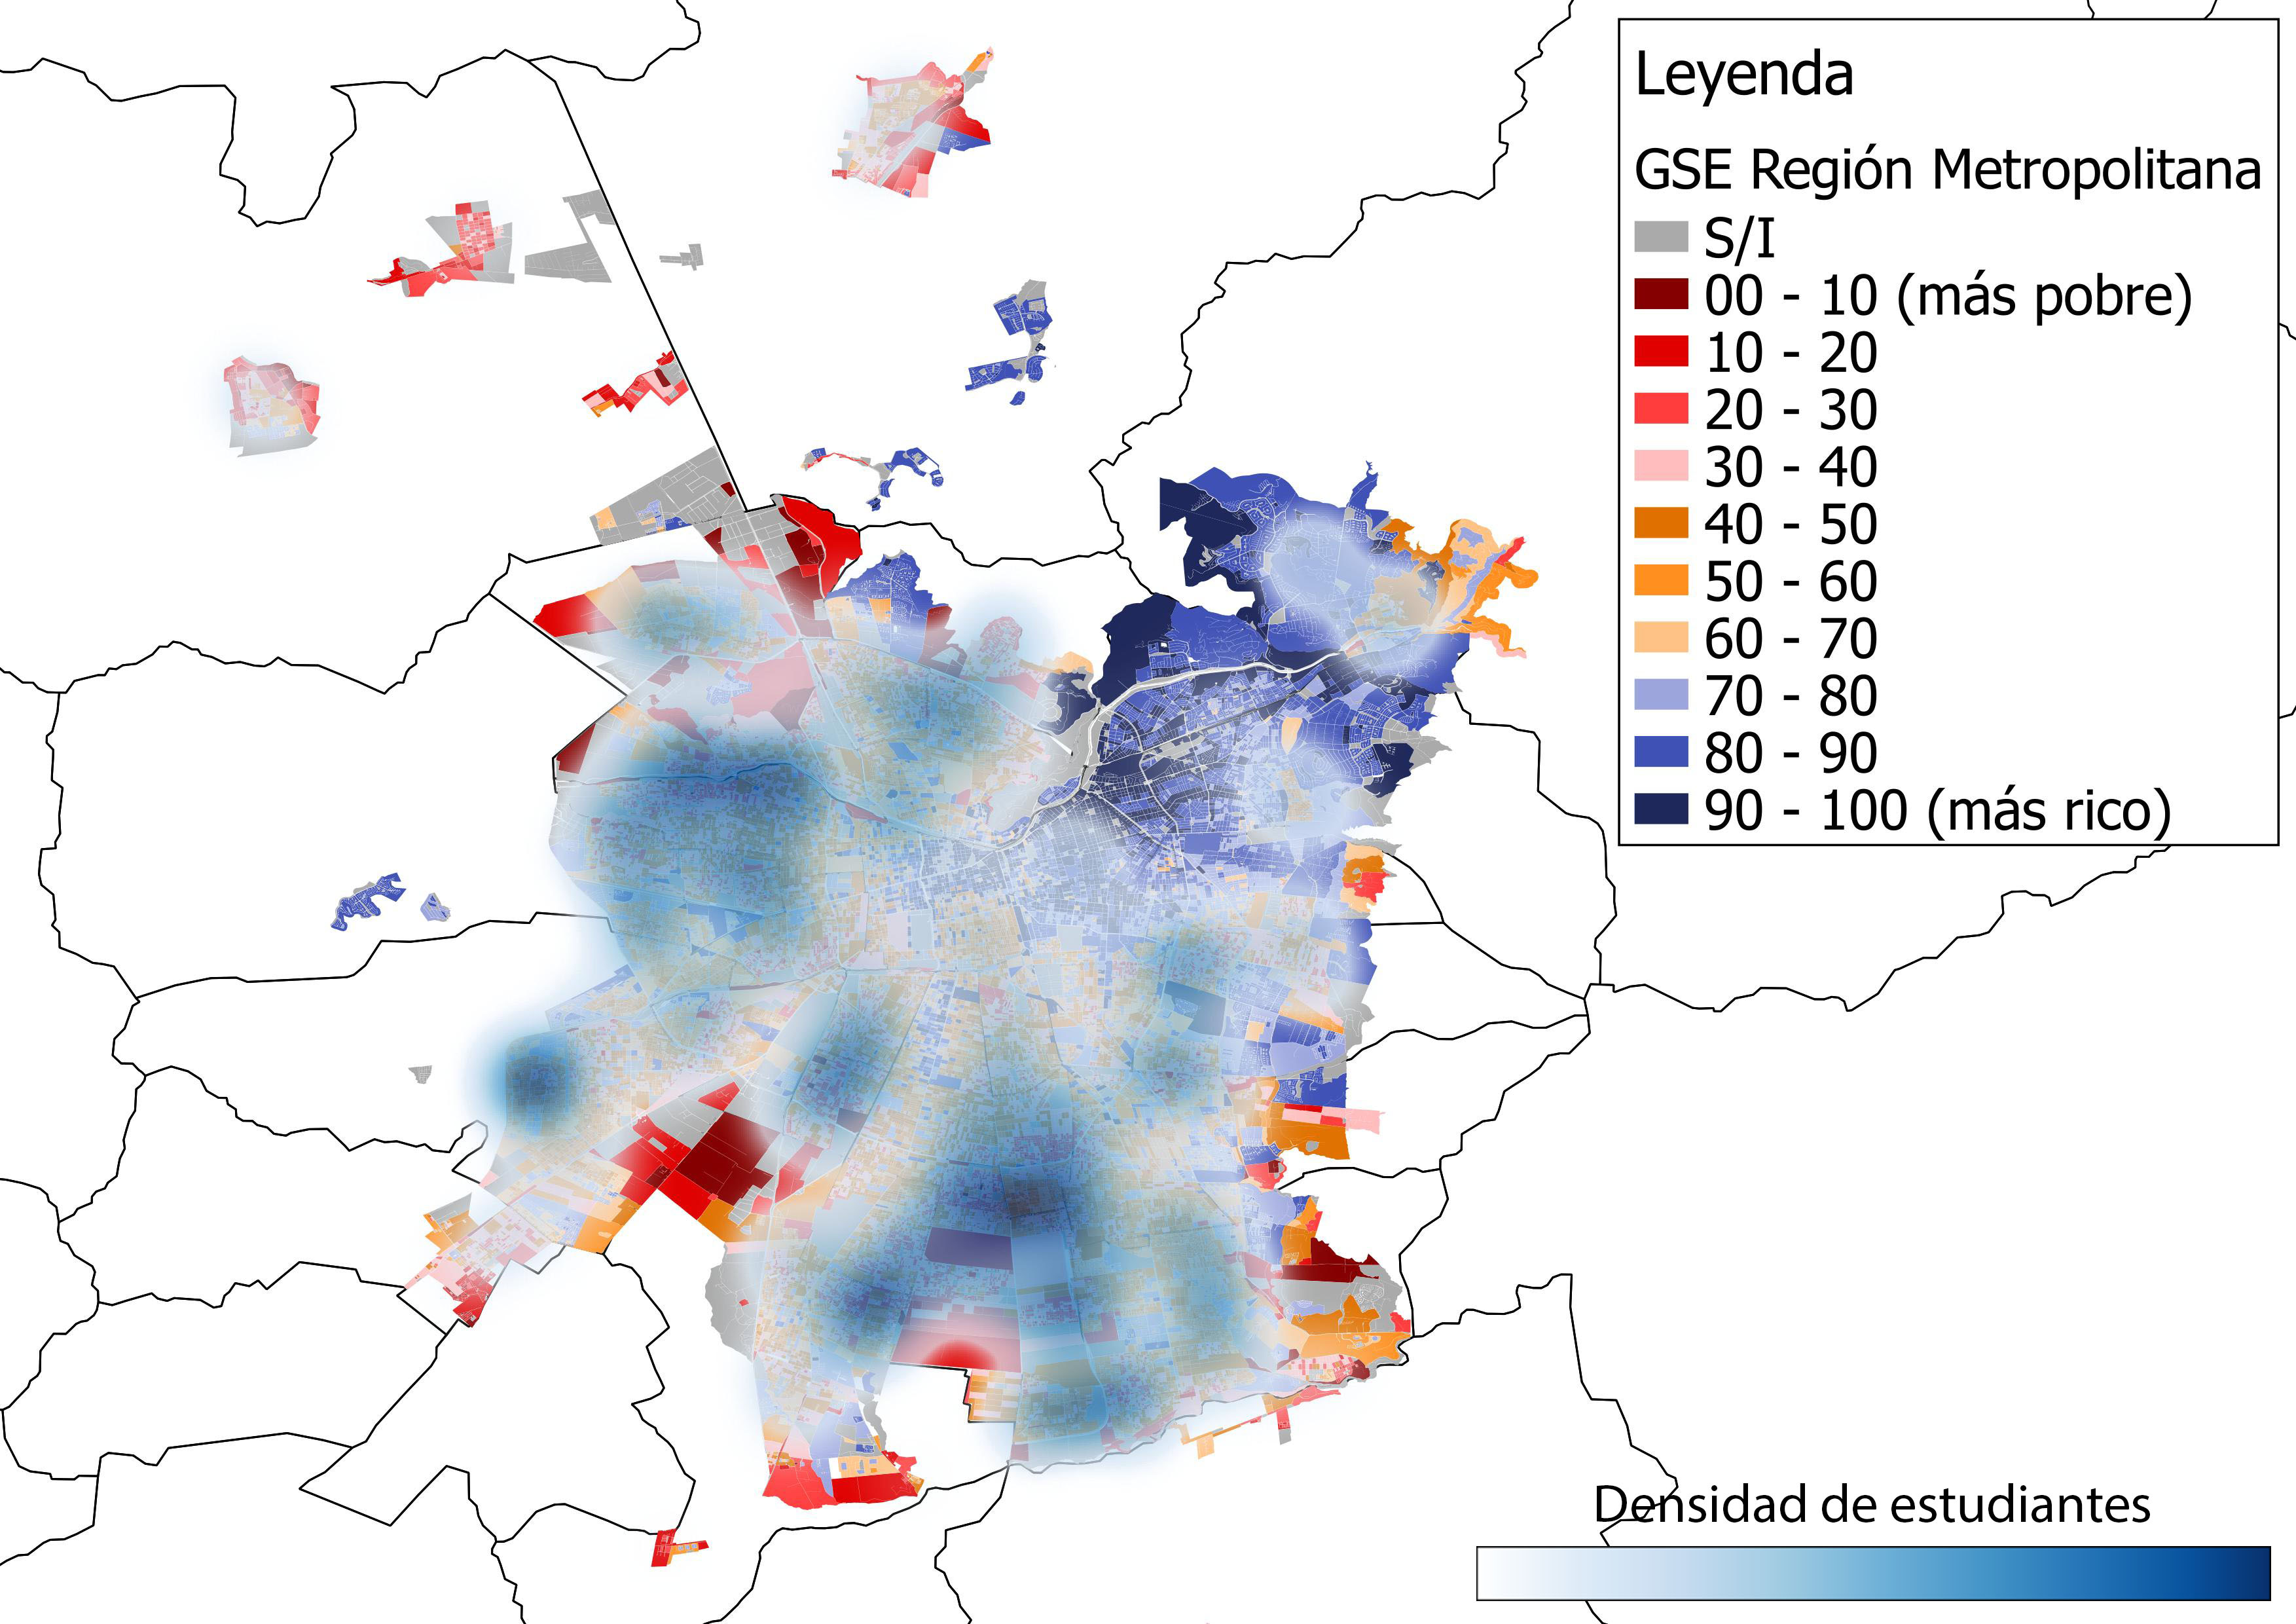
\includegraphics[width=7.5cm]{images/matriculas/E_CON_1_final.jpg}}\hspace{1mm}
  \subfloat[Matrículas en colegios de E\_TODOS\_CON\_2.]{
   \label{f:mapa_mat_en_estab_con_2_gse}
    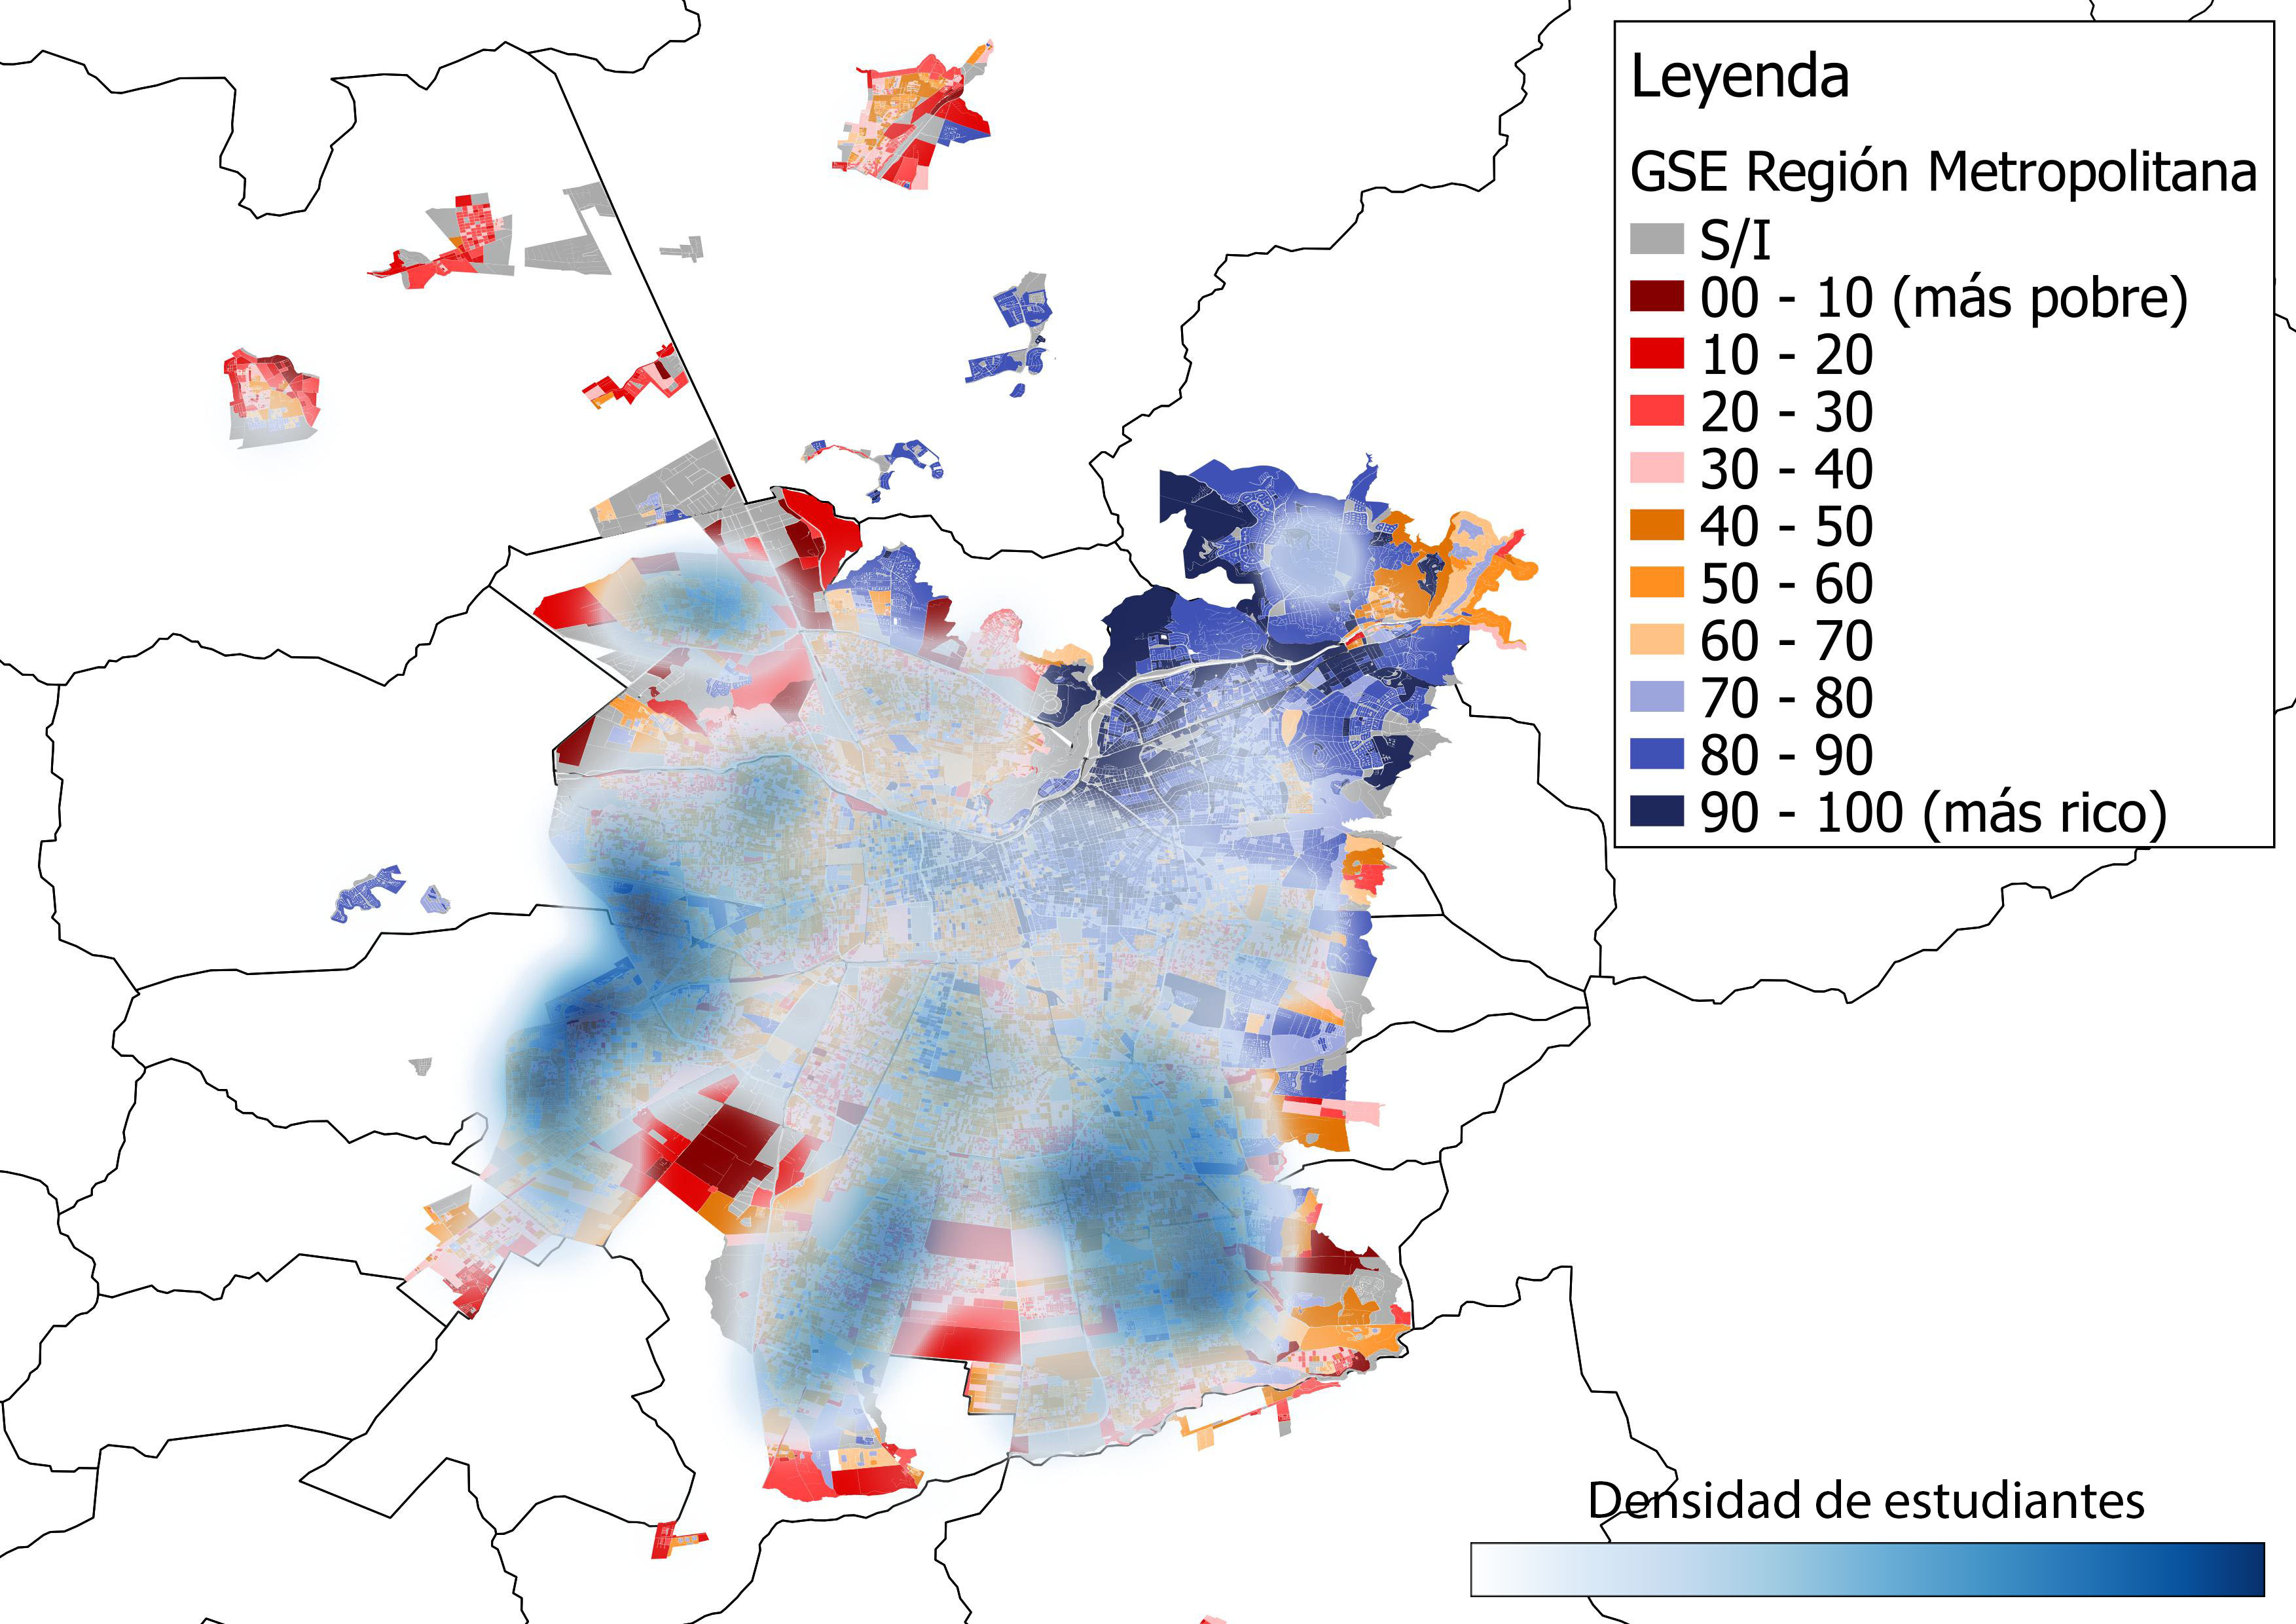
\includegraphics[width=7.5cm]{images/matriculas/E_CON_2_final.jpg}}
  \subfloat[Matrículas en colegios de E\_TODOS\_CON\_3.]{
   \label{f:mapa_mat_en_estab_con_3_gse}
    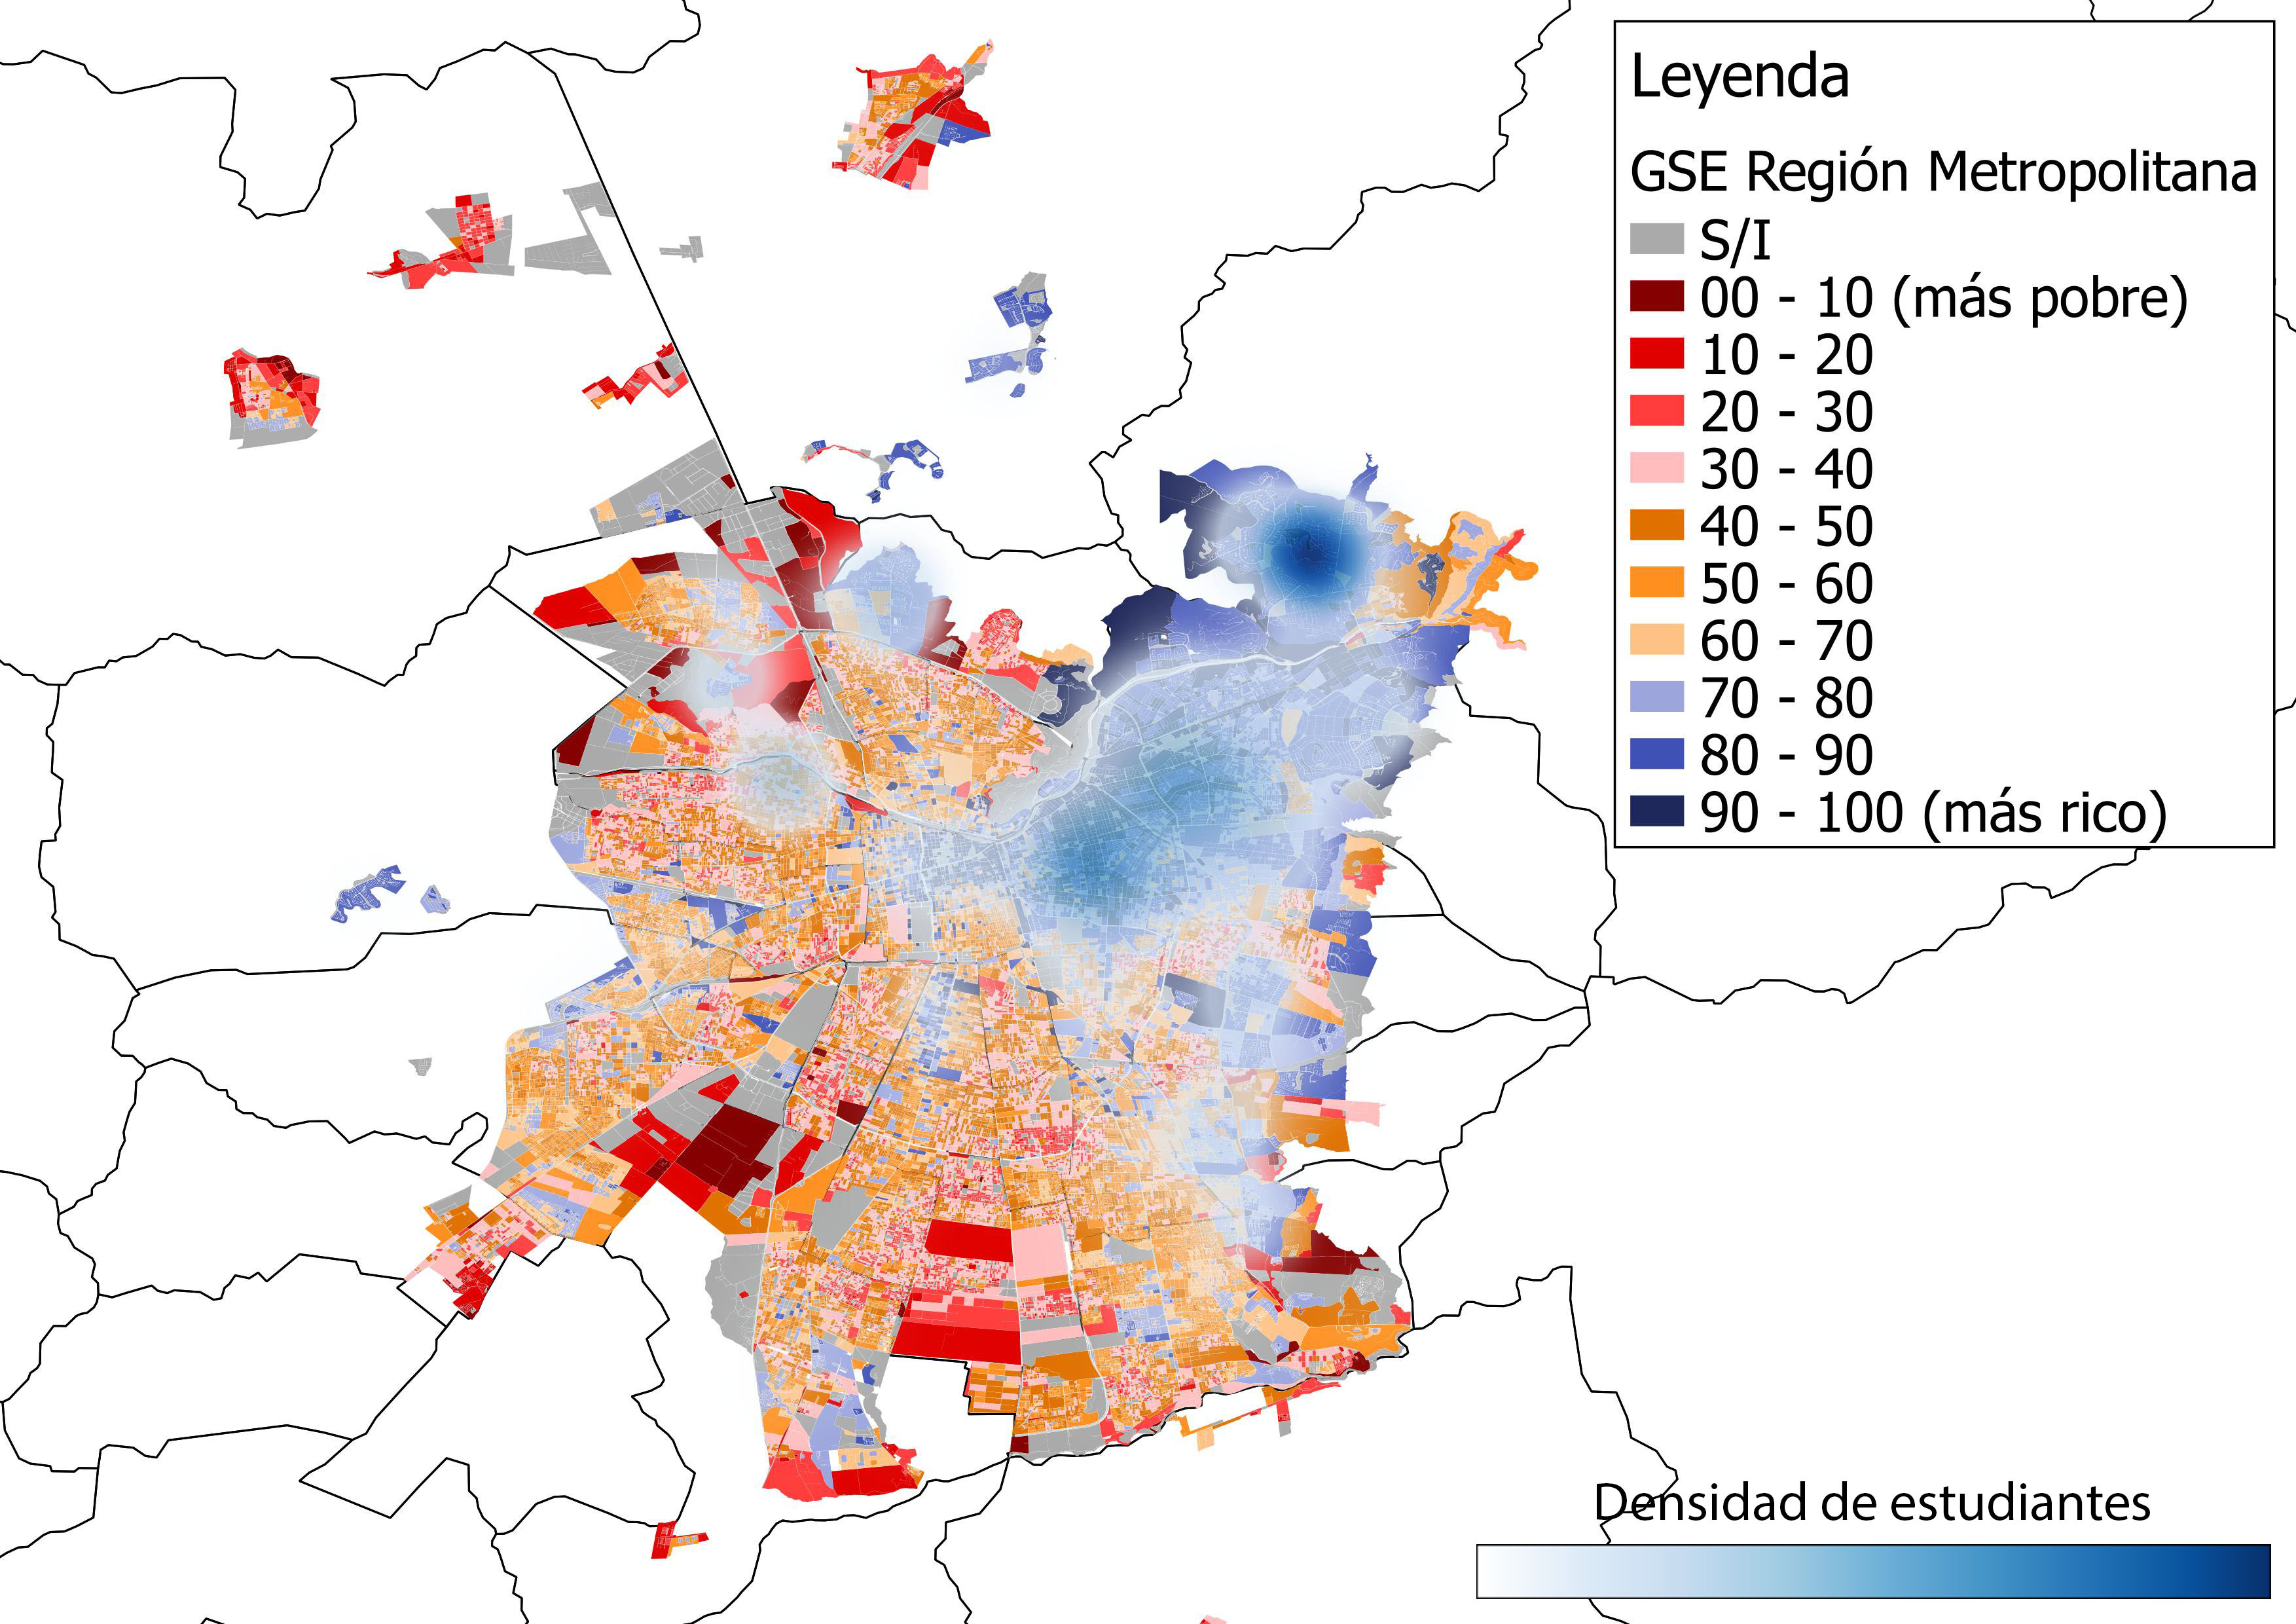
\includegraphics[width=7.5cm]{images/matriculas/E_CON_3_final.jpg}}
 \caption{Mapas de calor de matrículas (con atributos relacionales) en clústers de establecimientos sobre mapa GSE de la Región Metropolitana.}
 \label{f:mapas_mat_en_estab_con_gse}
\end{figure}

En las imágenes \ref{f:mapas_mat_sin_gse} y \ref{f:mapas_mat_con_gse} se analizan las distribuciones de los clústers de estudiantes dentro del área metropolitana y sus diferentes grupos socioeconómicos, con y sin considerar sus variables de relación establecimiento - matrícula. En las figuras \ref{f:mapa_mat_sin_0_gse} y \ref{f:mapa_mat_sin_1_gse} se aprecia que los estudiantes están dispersos por casi toda el área metropolitana, en menor medida en el sector oriente y con grandes concentraciones en el sector sur y poniente. Por otro lado, en las figuras \ref{f:mapa_mat_sin_2_gse} y \ref{f:mapa_mat_sin_3_gse} si se distribuyen por toda el área metropolitana, con varios lugares de alta densidad, destacando como punto máximo la periferia del sector oriente.

Al analizar los grupos socioeconómicos en los cuales se encuentran, los primeros dos están presentes en los deciles del 4 al 7 principalmente y los otros dos en los deciles del 4 al 10, donde su \textit{peak} está en los deciles del 8 al 10.


\begin{figure}[H]
 \centering
  \subfloat[Matrículas clúster M\_TODAS\_SIN\_0.]{
   \label{f:mapa_mat_sin_0_gse}
    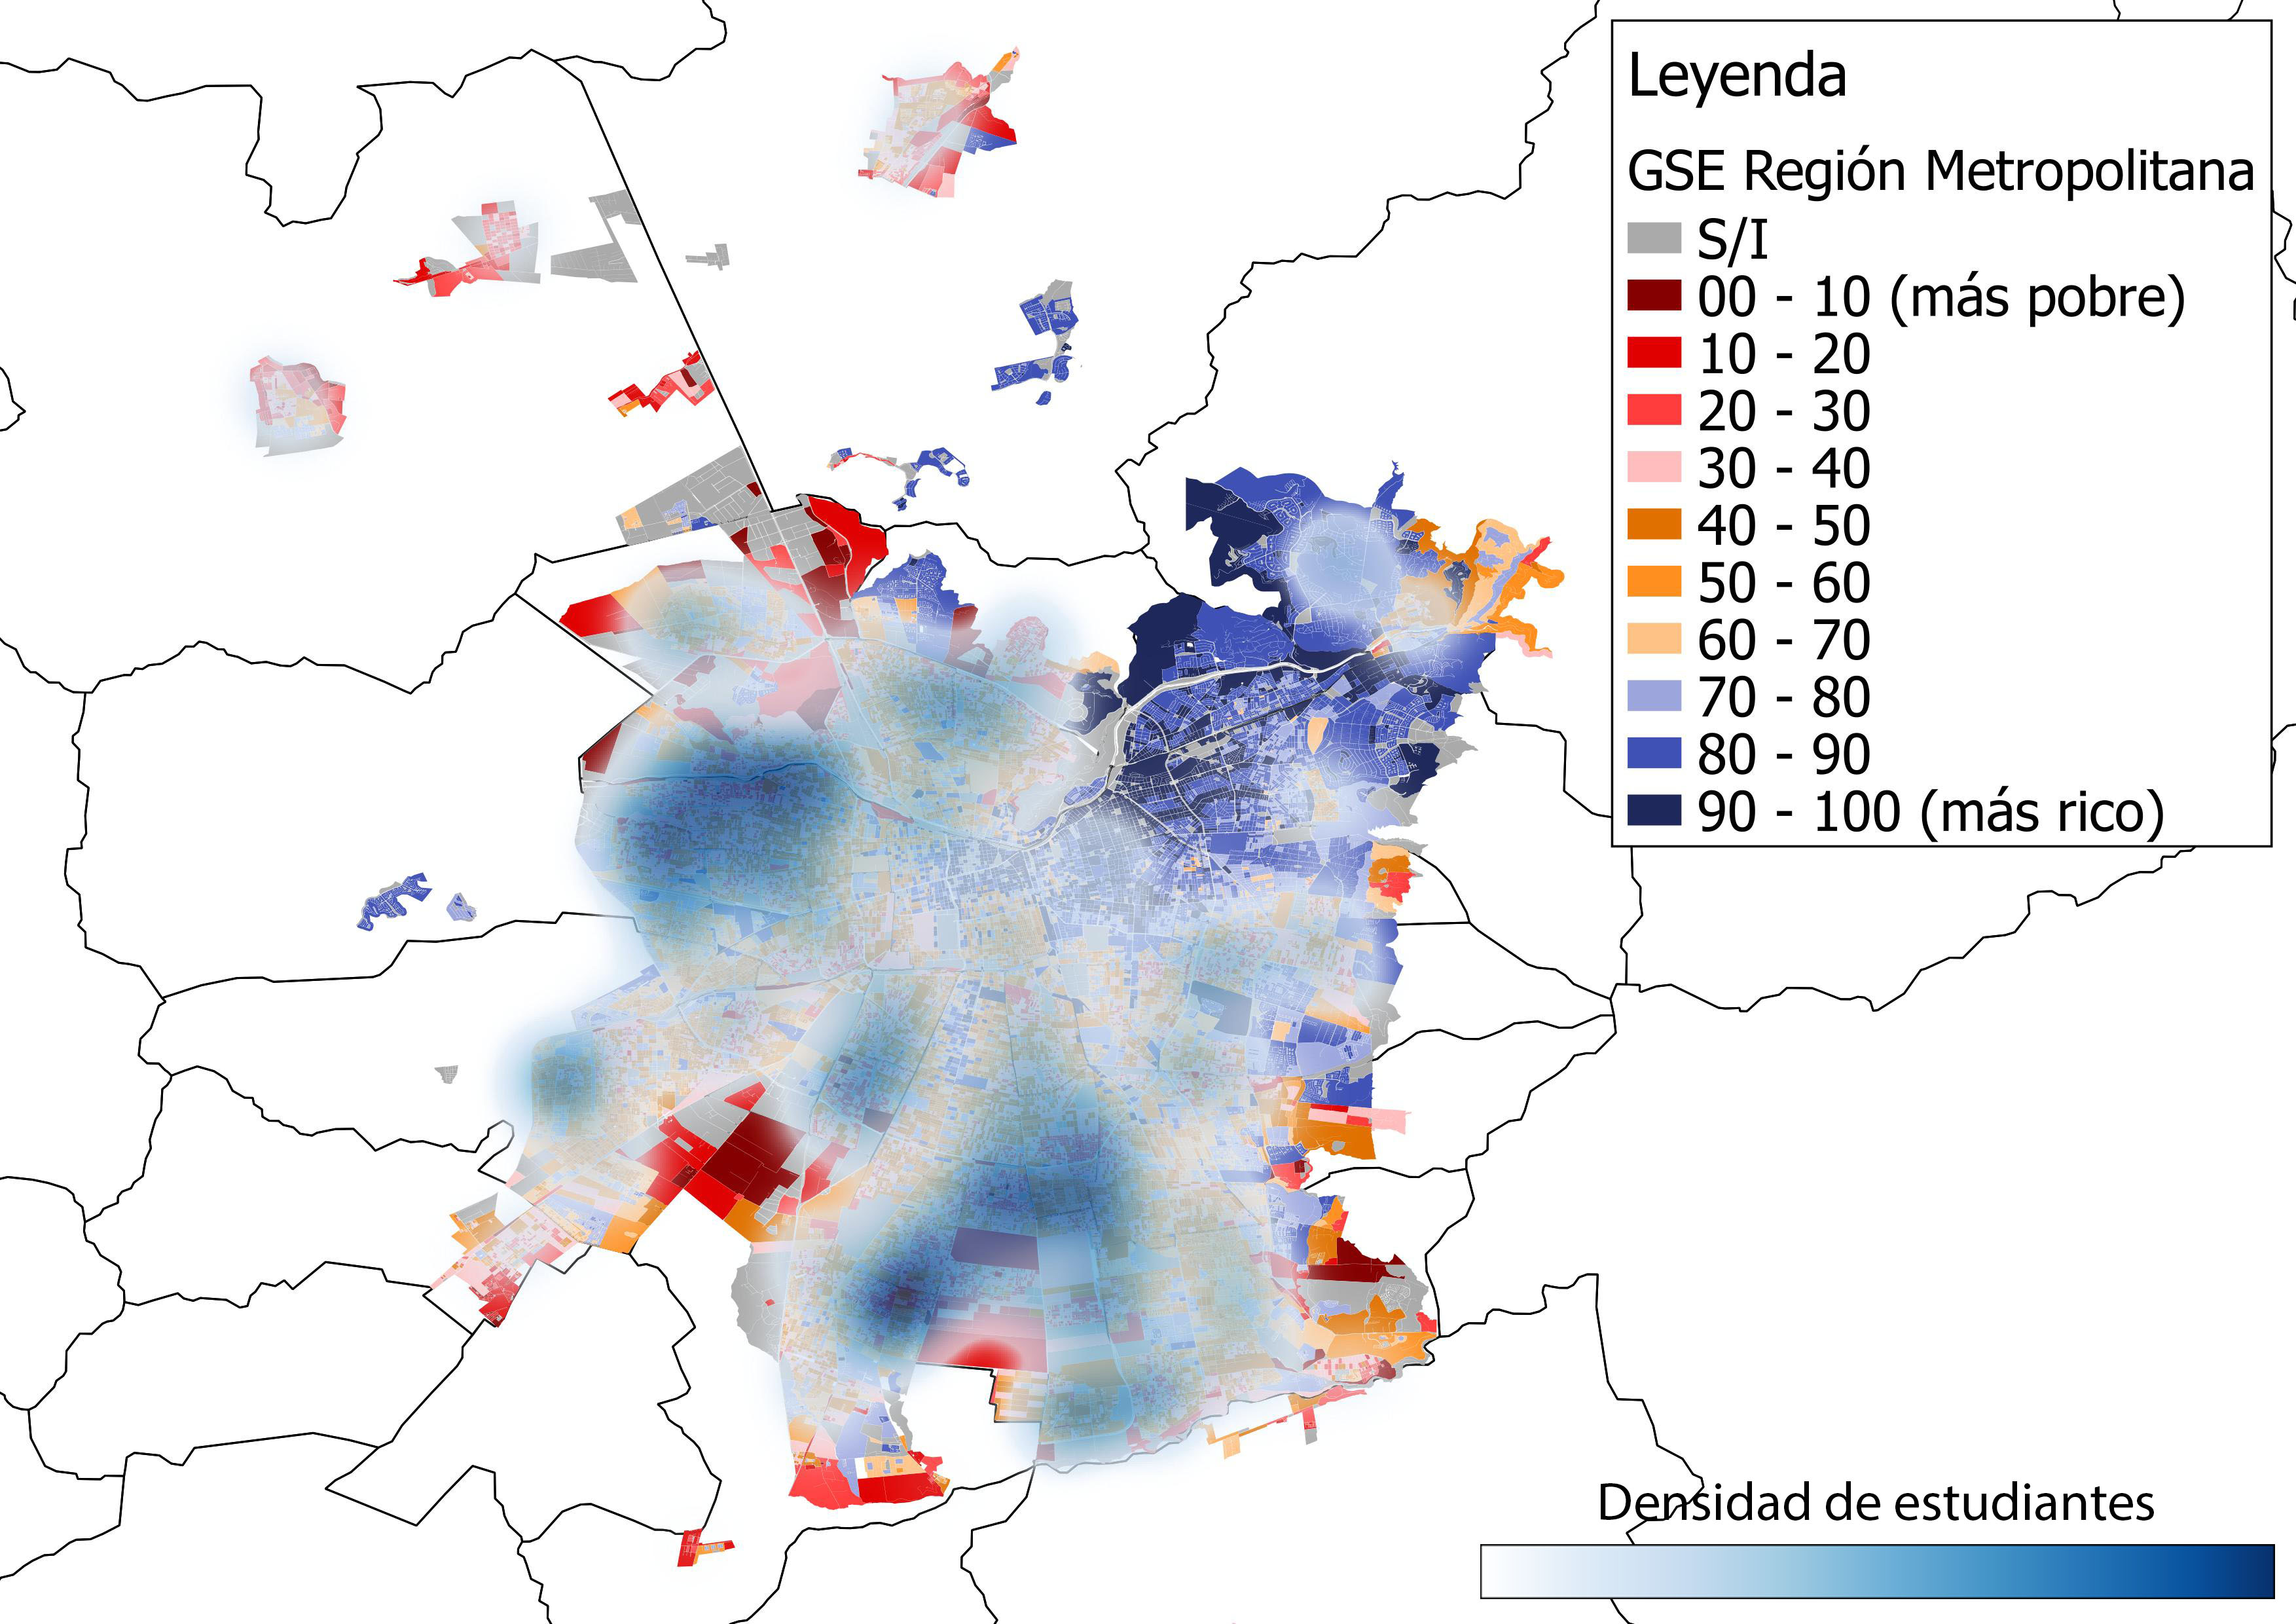
\includegraphics[width=7.5cm]{images/matriculas/M_SIN_0_final.jpg}}
  \subfloat[Matrículas clúster M\_TODAS\_SIN\_1.]{
   \label{f:mapa_mat_sin_1_gse}
    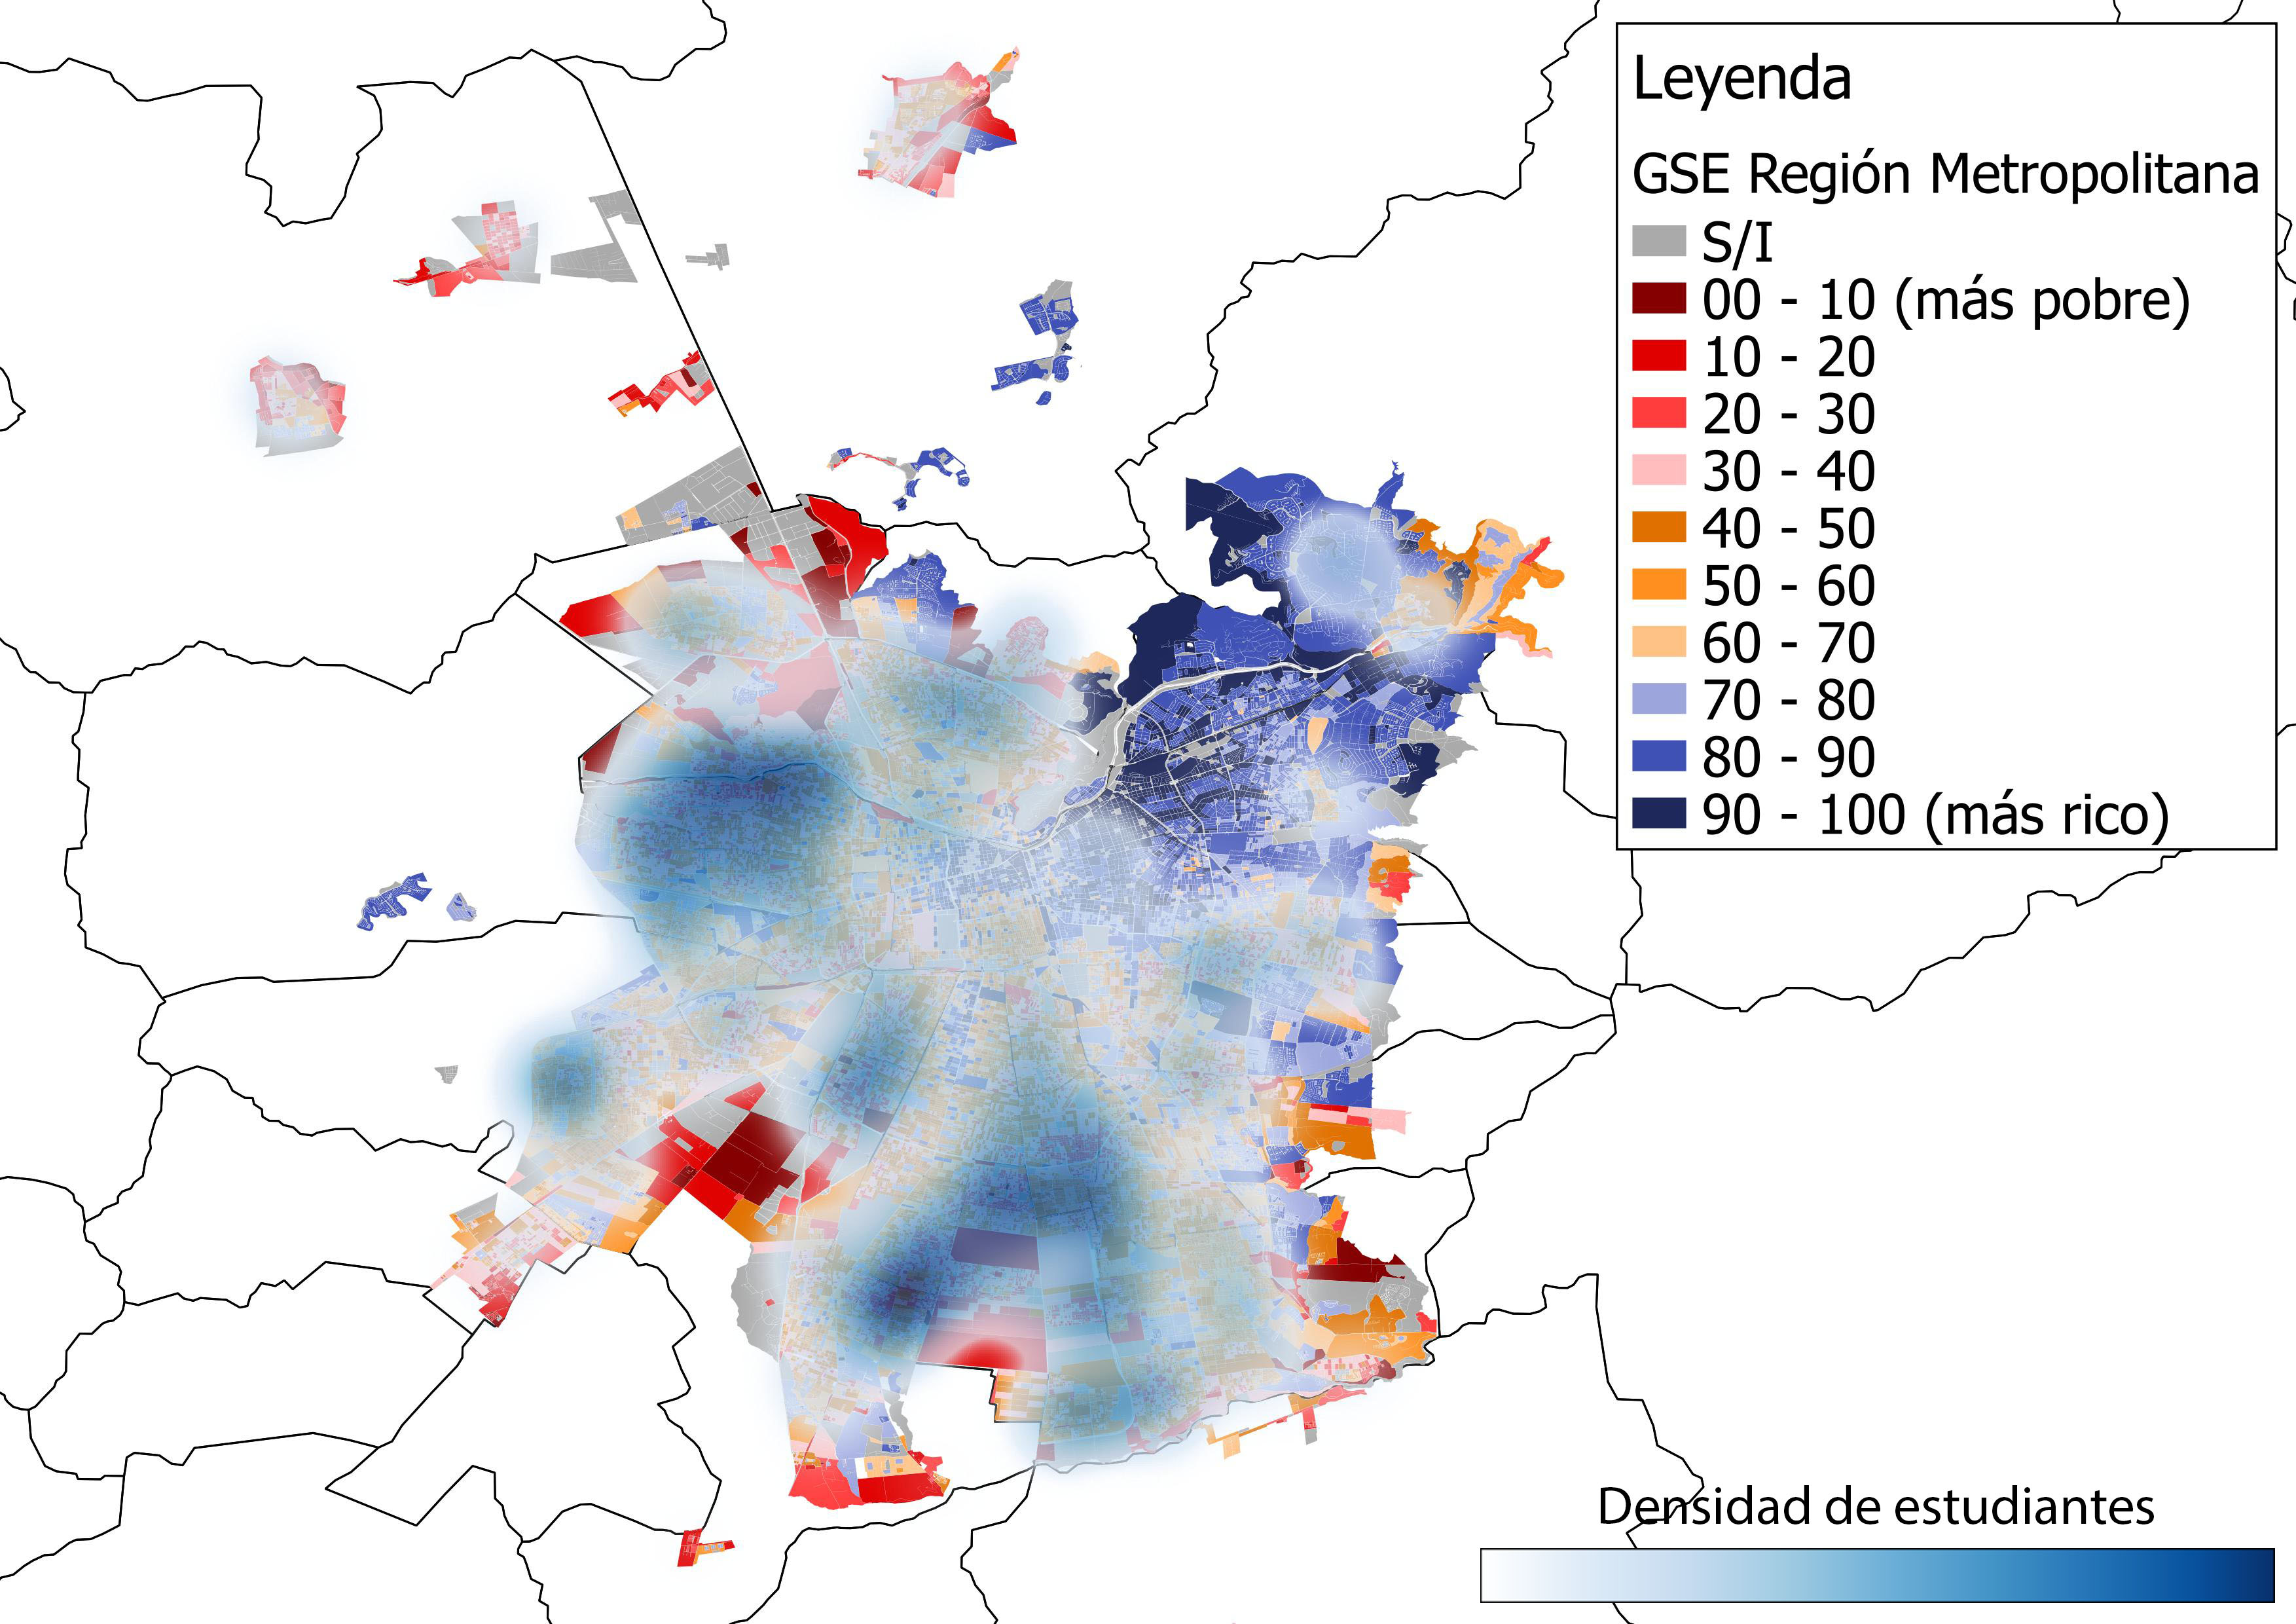
\includegraphics[width=7.5cm]{images/matriculas/M_SIN_1_final.jpg}}\hspace{1mm}
  \subfloat[Matrículas clúster M\_TODAS\_SIN\_2.]{
   \label{f:mapa_mat_sin_2_gse}
    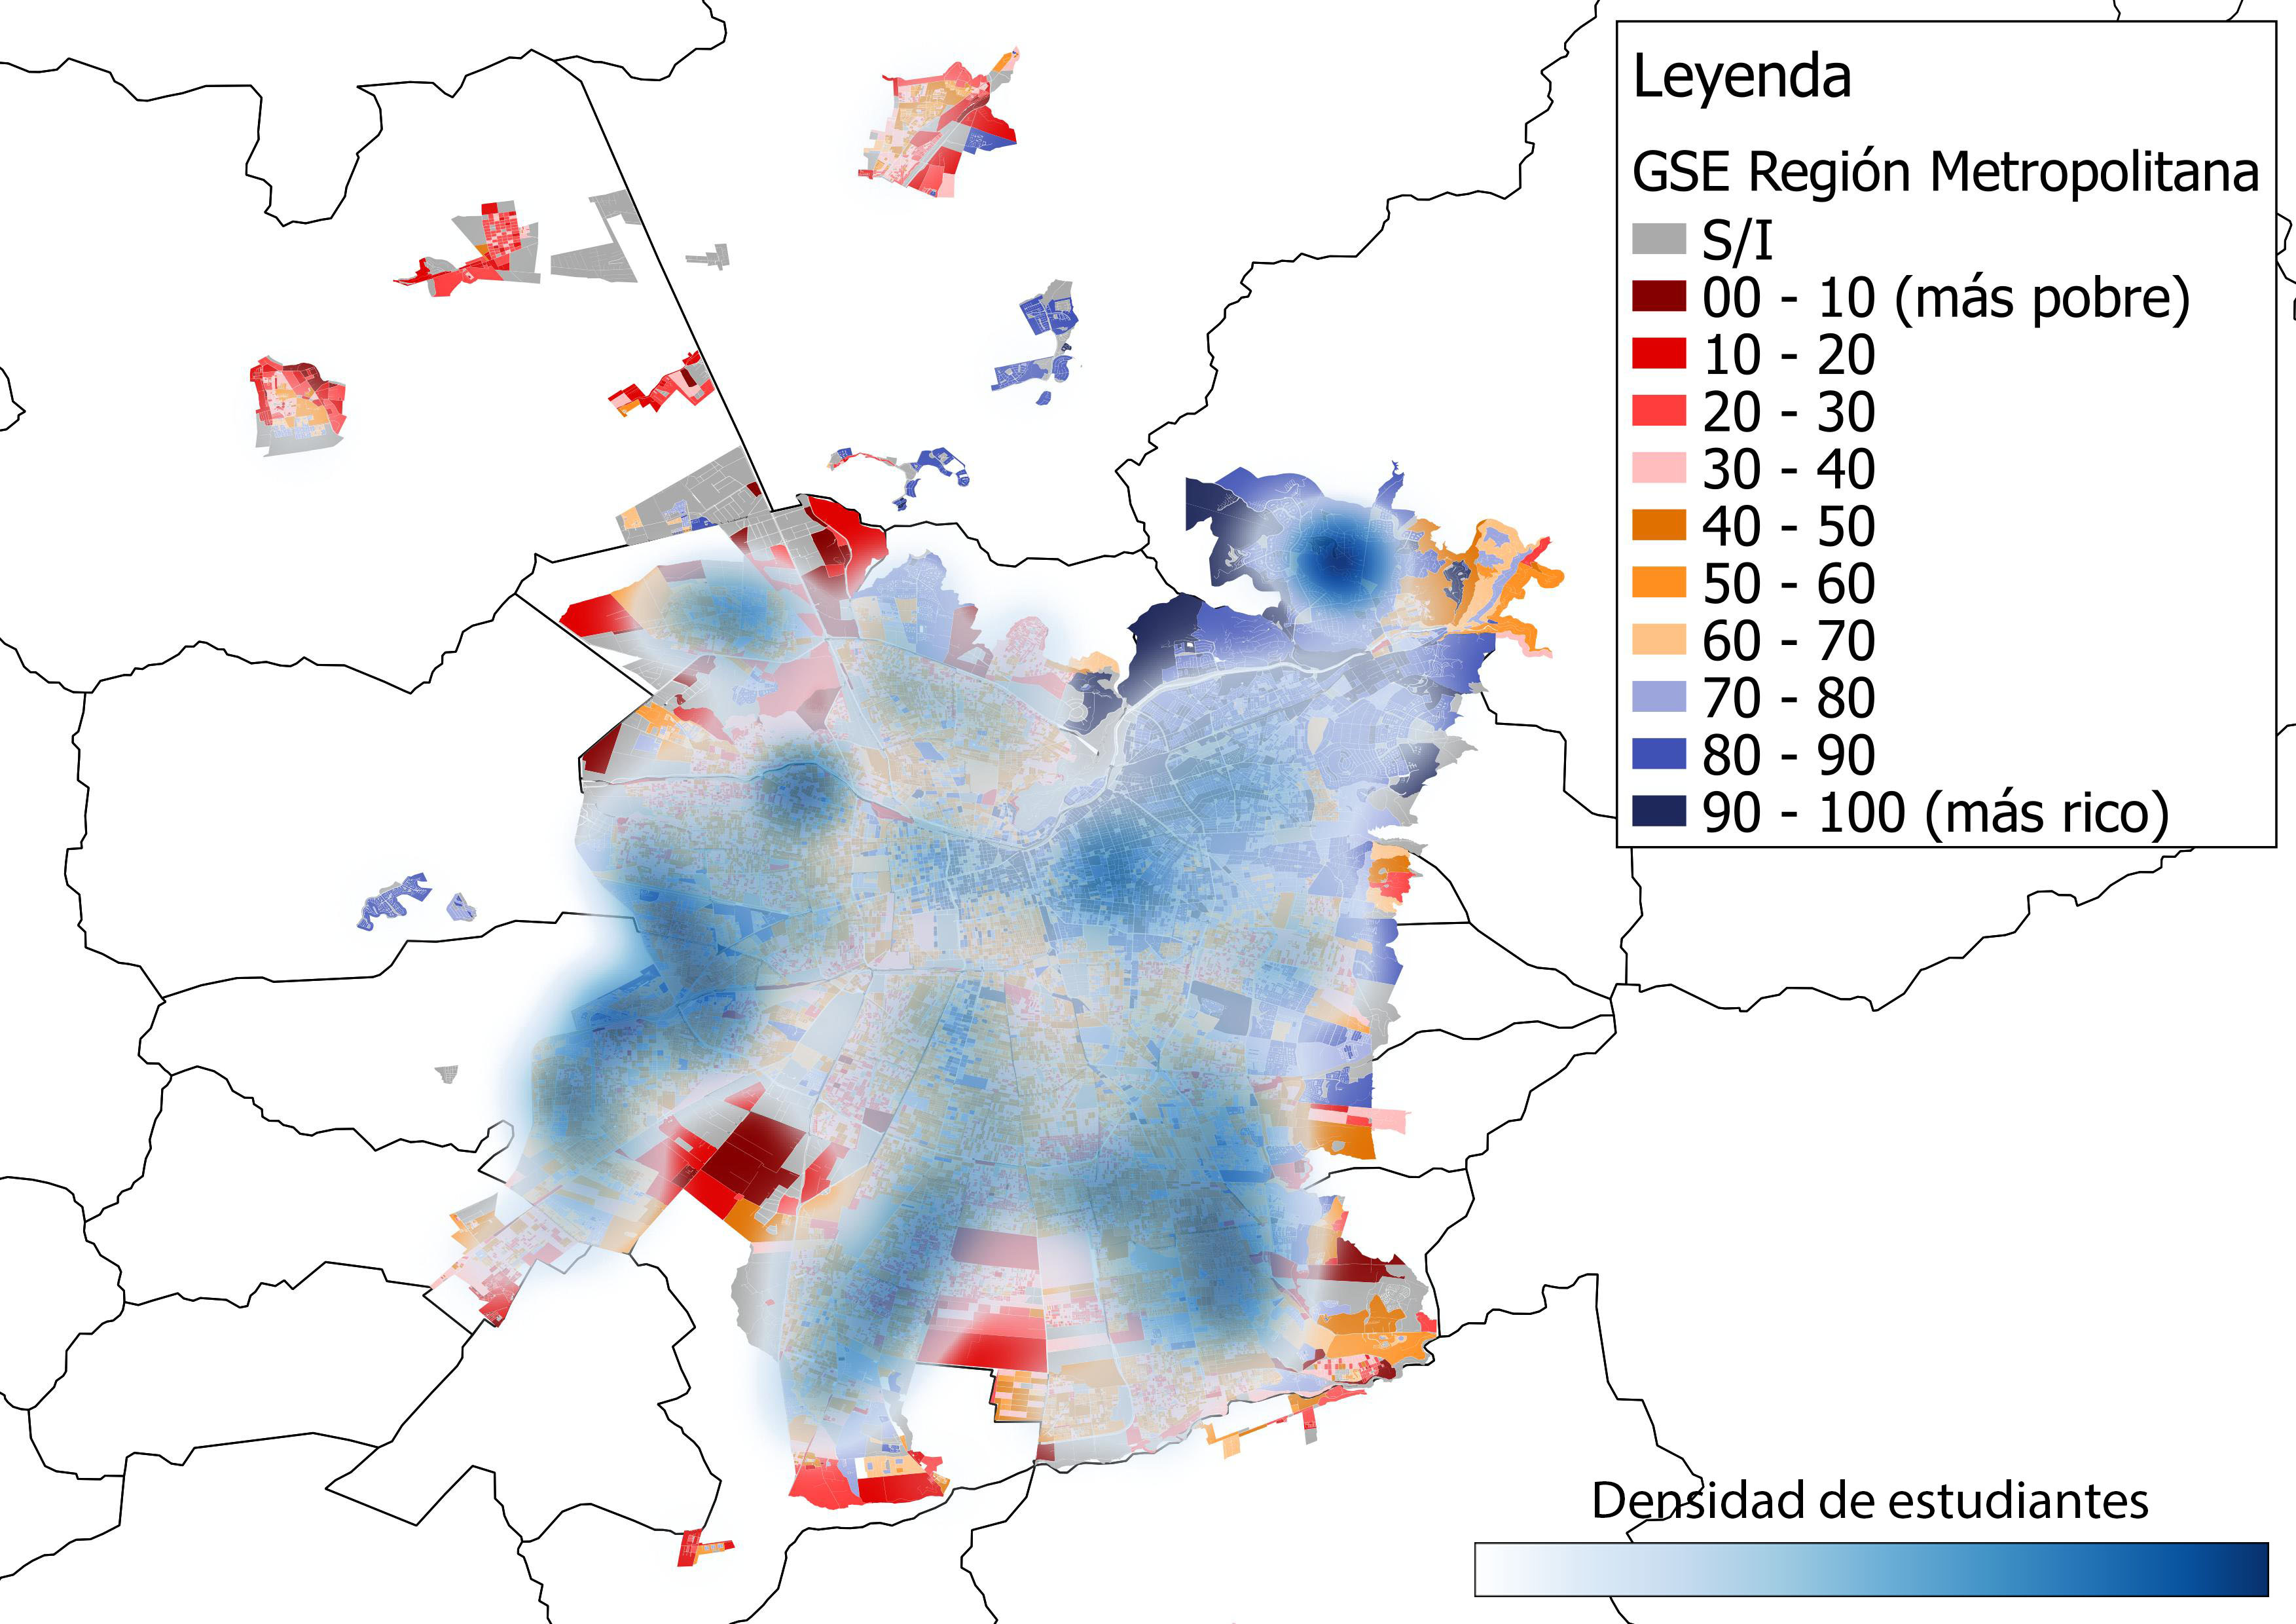
\includegraphics[width=7.5cm]{images/matriculas/M_SIN_2_final.jpg}}
  \subfloat[Matrículas clúster M\_TODAS\_SIN\_3.]{
   \label{f:mapa_mat_sin_3_gse}
    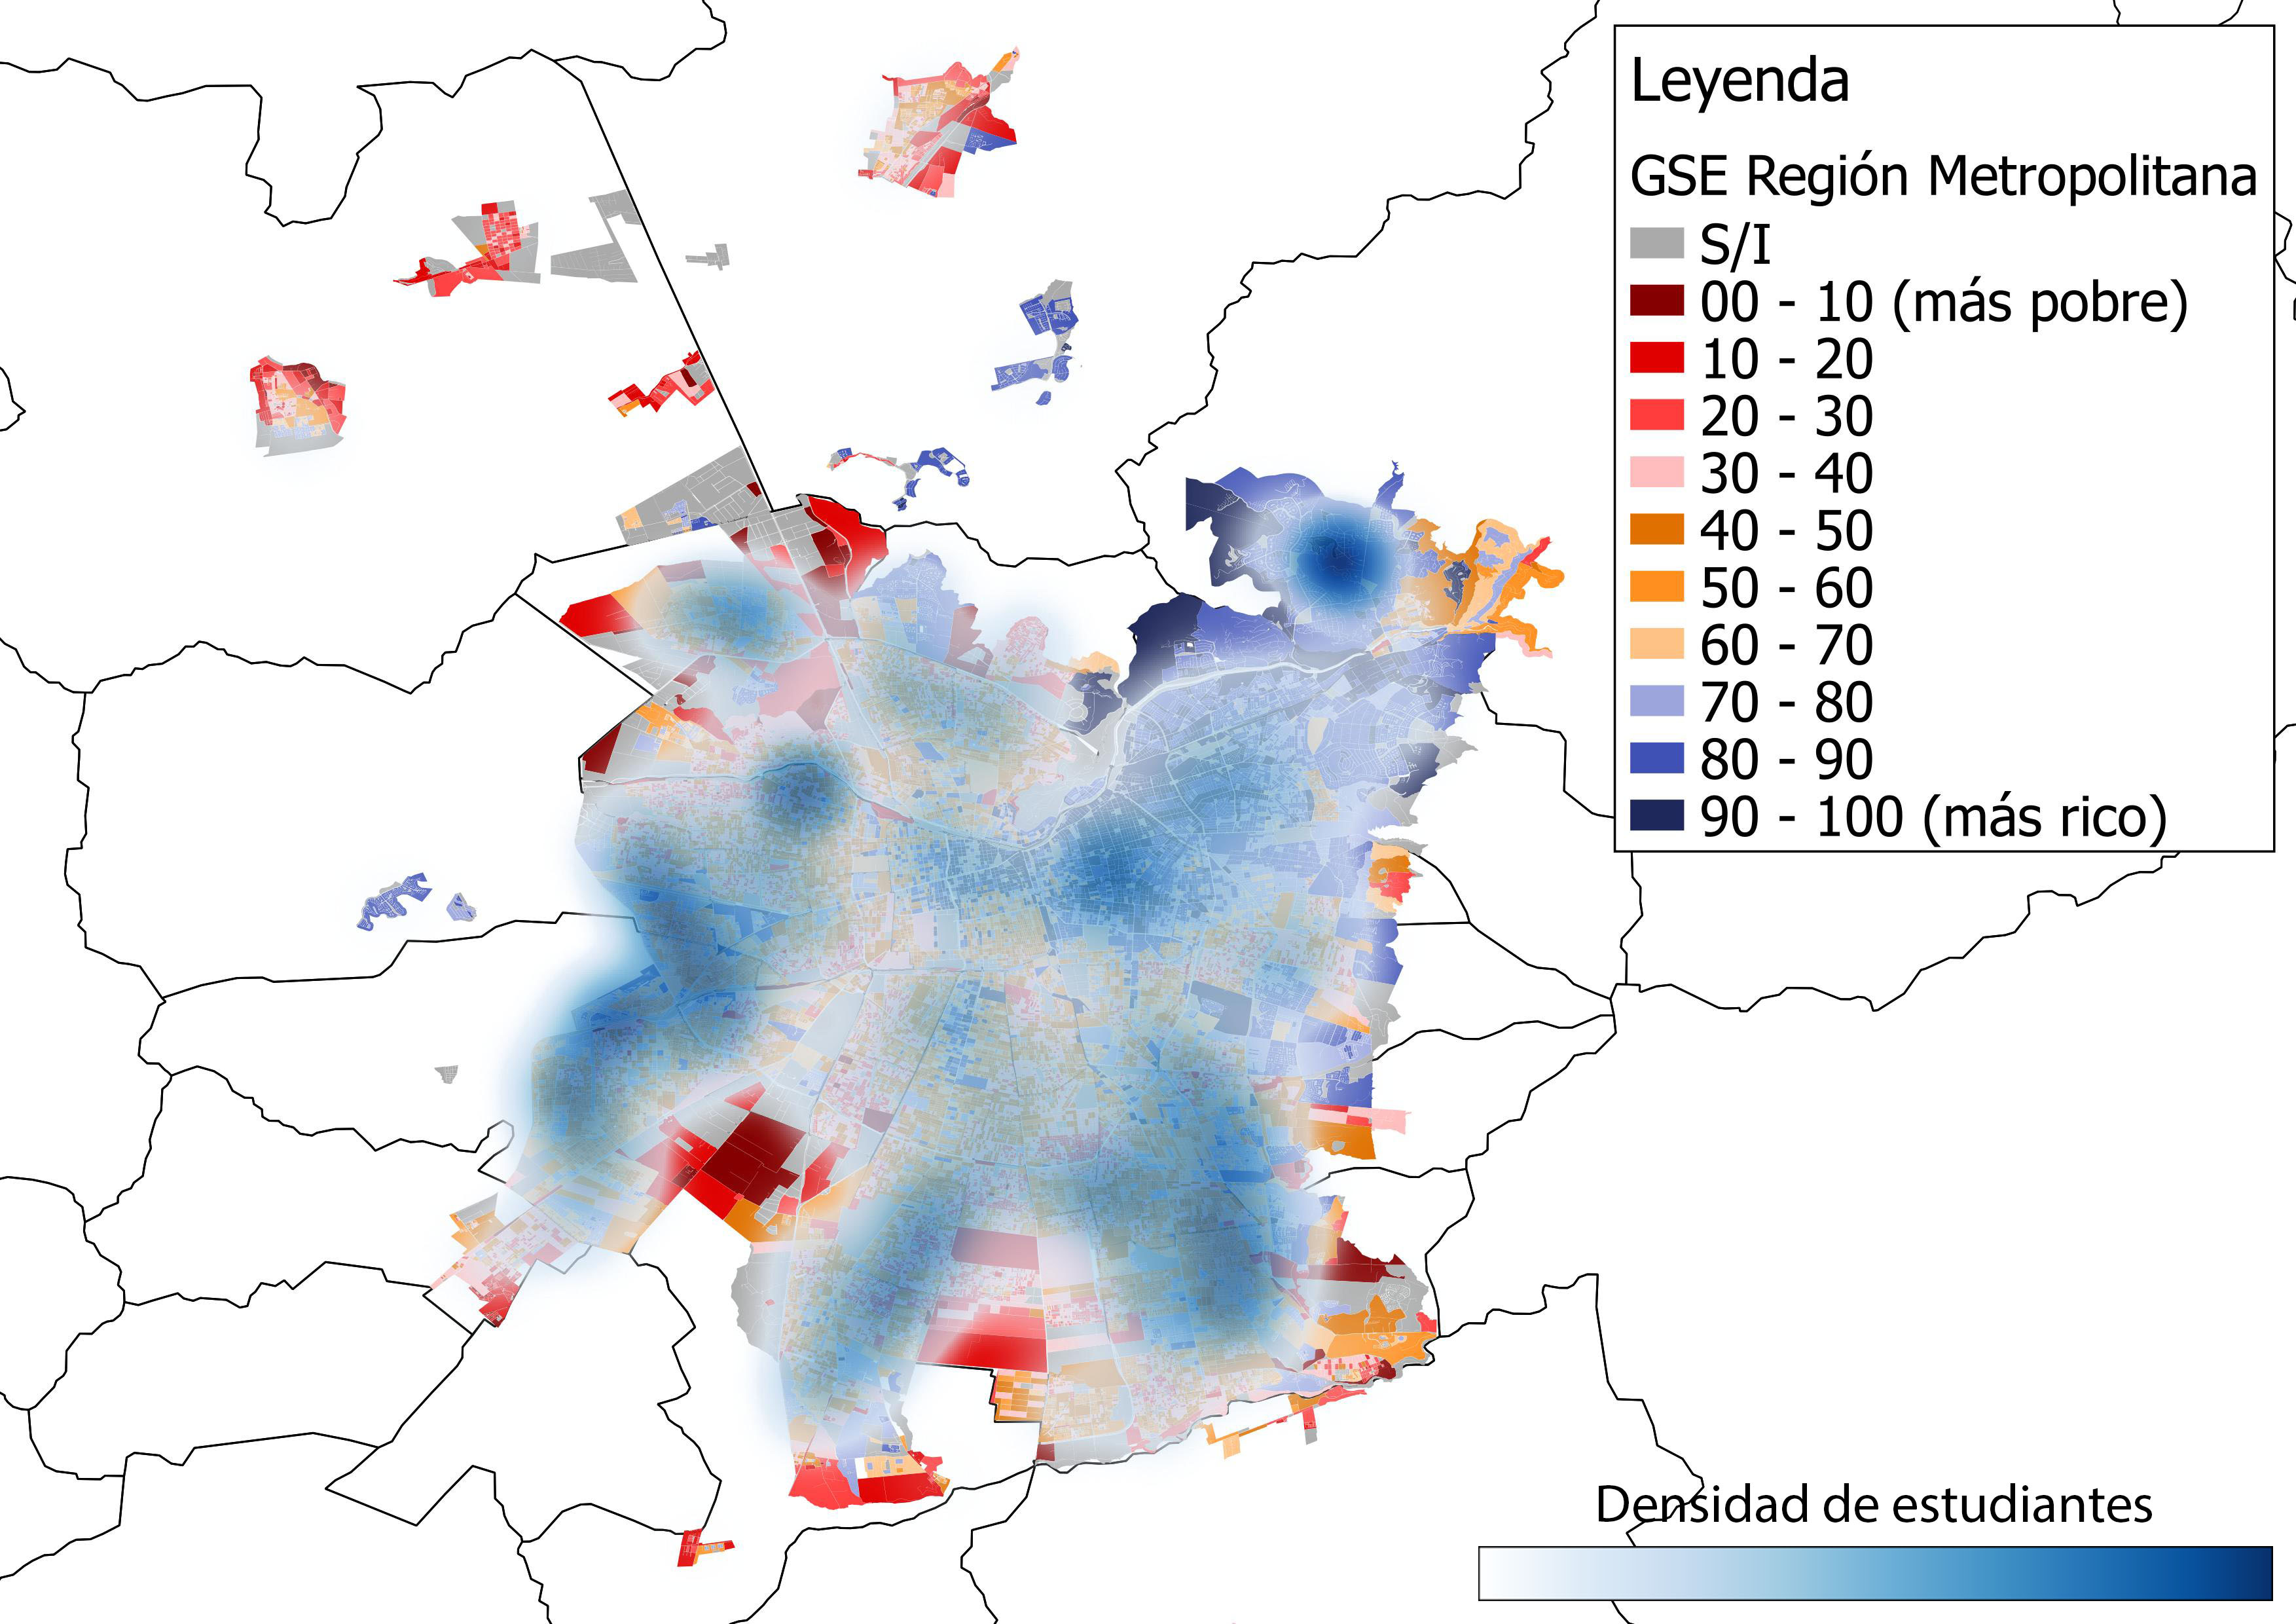
\includegraphics[width=7.5cm]{images/matriculas/M_SIN_3_final.jpg}}
 \caption{Mapas de calor de clústers de matrículas sobre mapa GSE de la Región Metropolitana.}
 \label{f:mapas_mat_sin_gse}
\end{figure}

Al analizar las imágenes \ref{f:mapa_mat_con_0_gse} y \ref{f:mapa_mat_con_1_gse} podemos observar una gran similitud, en donde los alumnos se distribuyen por casi toda el área metropolitana, pero disminuye notoriamente en el sector oriente. En la figura \ref{f:mapa_mat_con_2_gse} encontramos alumnos en casi toda el área metropolitana, pero las zonas donde más se concentran los estudiantes es el sector sur y poniente. Por último, en \ref{f:mapa_mat_con_3_gse}, casi todos los alumnos residen en el sector oriente de la capital, siendo la periferia de este donde existe una mayor concentración.

A diferencia del análisis sin variables de relación, las primeras 3 figuras muestran que los alumnos viven en sectores socioeconómicos que van del decil 2 al decil 8, es decir, comprenden grupos muy variados. Caso aparte es la última imagen, donde los estudiantes residen en sectores pertencientes a los deciles del 8 al 10.

\begin{figure}[H]
 \centering
  \subfloat[Matrículas clúster M\_TODAS\_CON\_0.]{
   \label{f:mapa_mat_con_0_gse}
    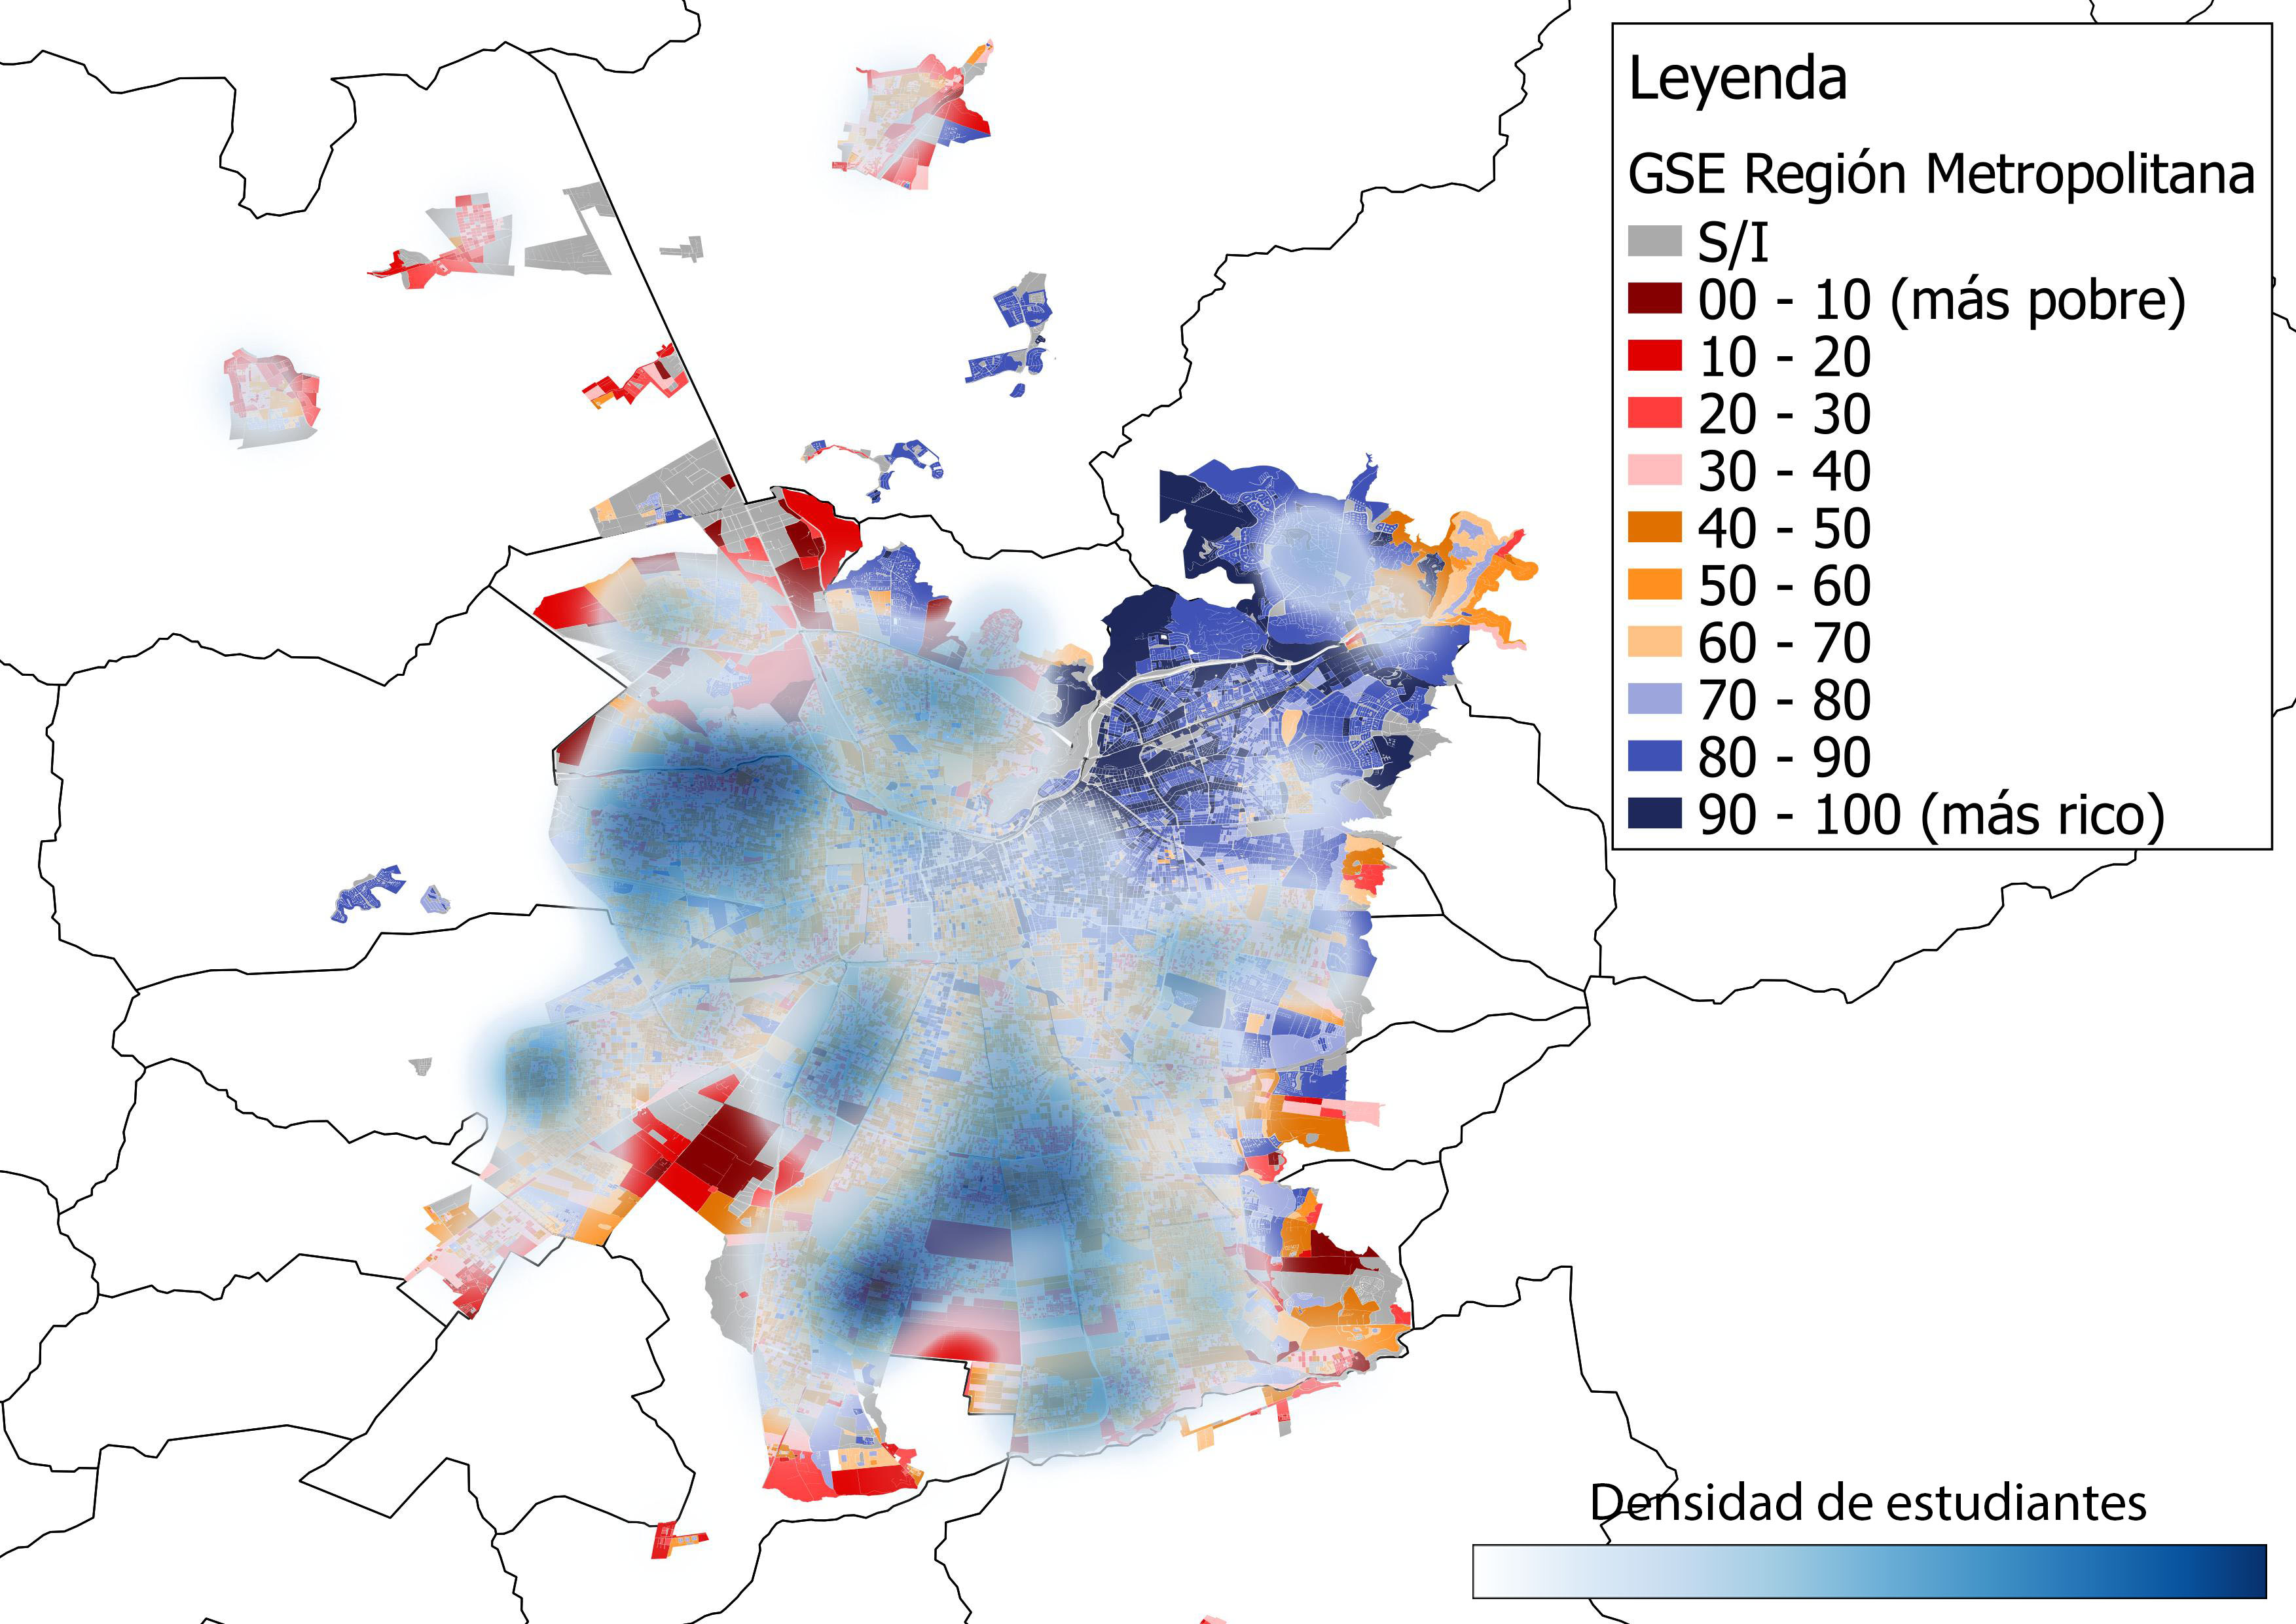
\includegraphics[width=7.5cm]{images/matriculas/M_CON_0_final.jpg}}
  \subfloat[Matrículas clúster M\_TODAS\_CON\_1.]{
   \label{f:mapa_mat_con_1_gse}
    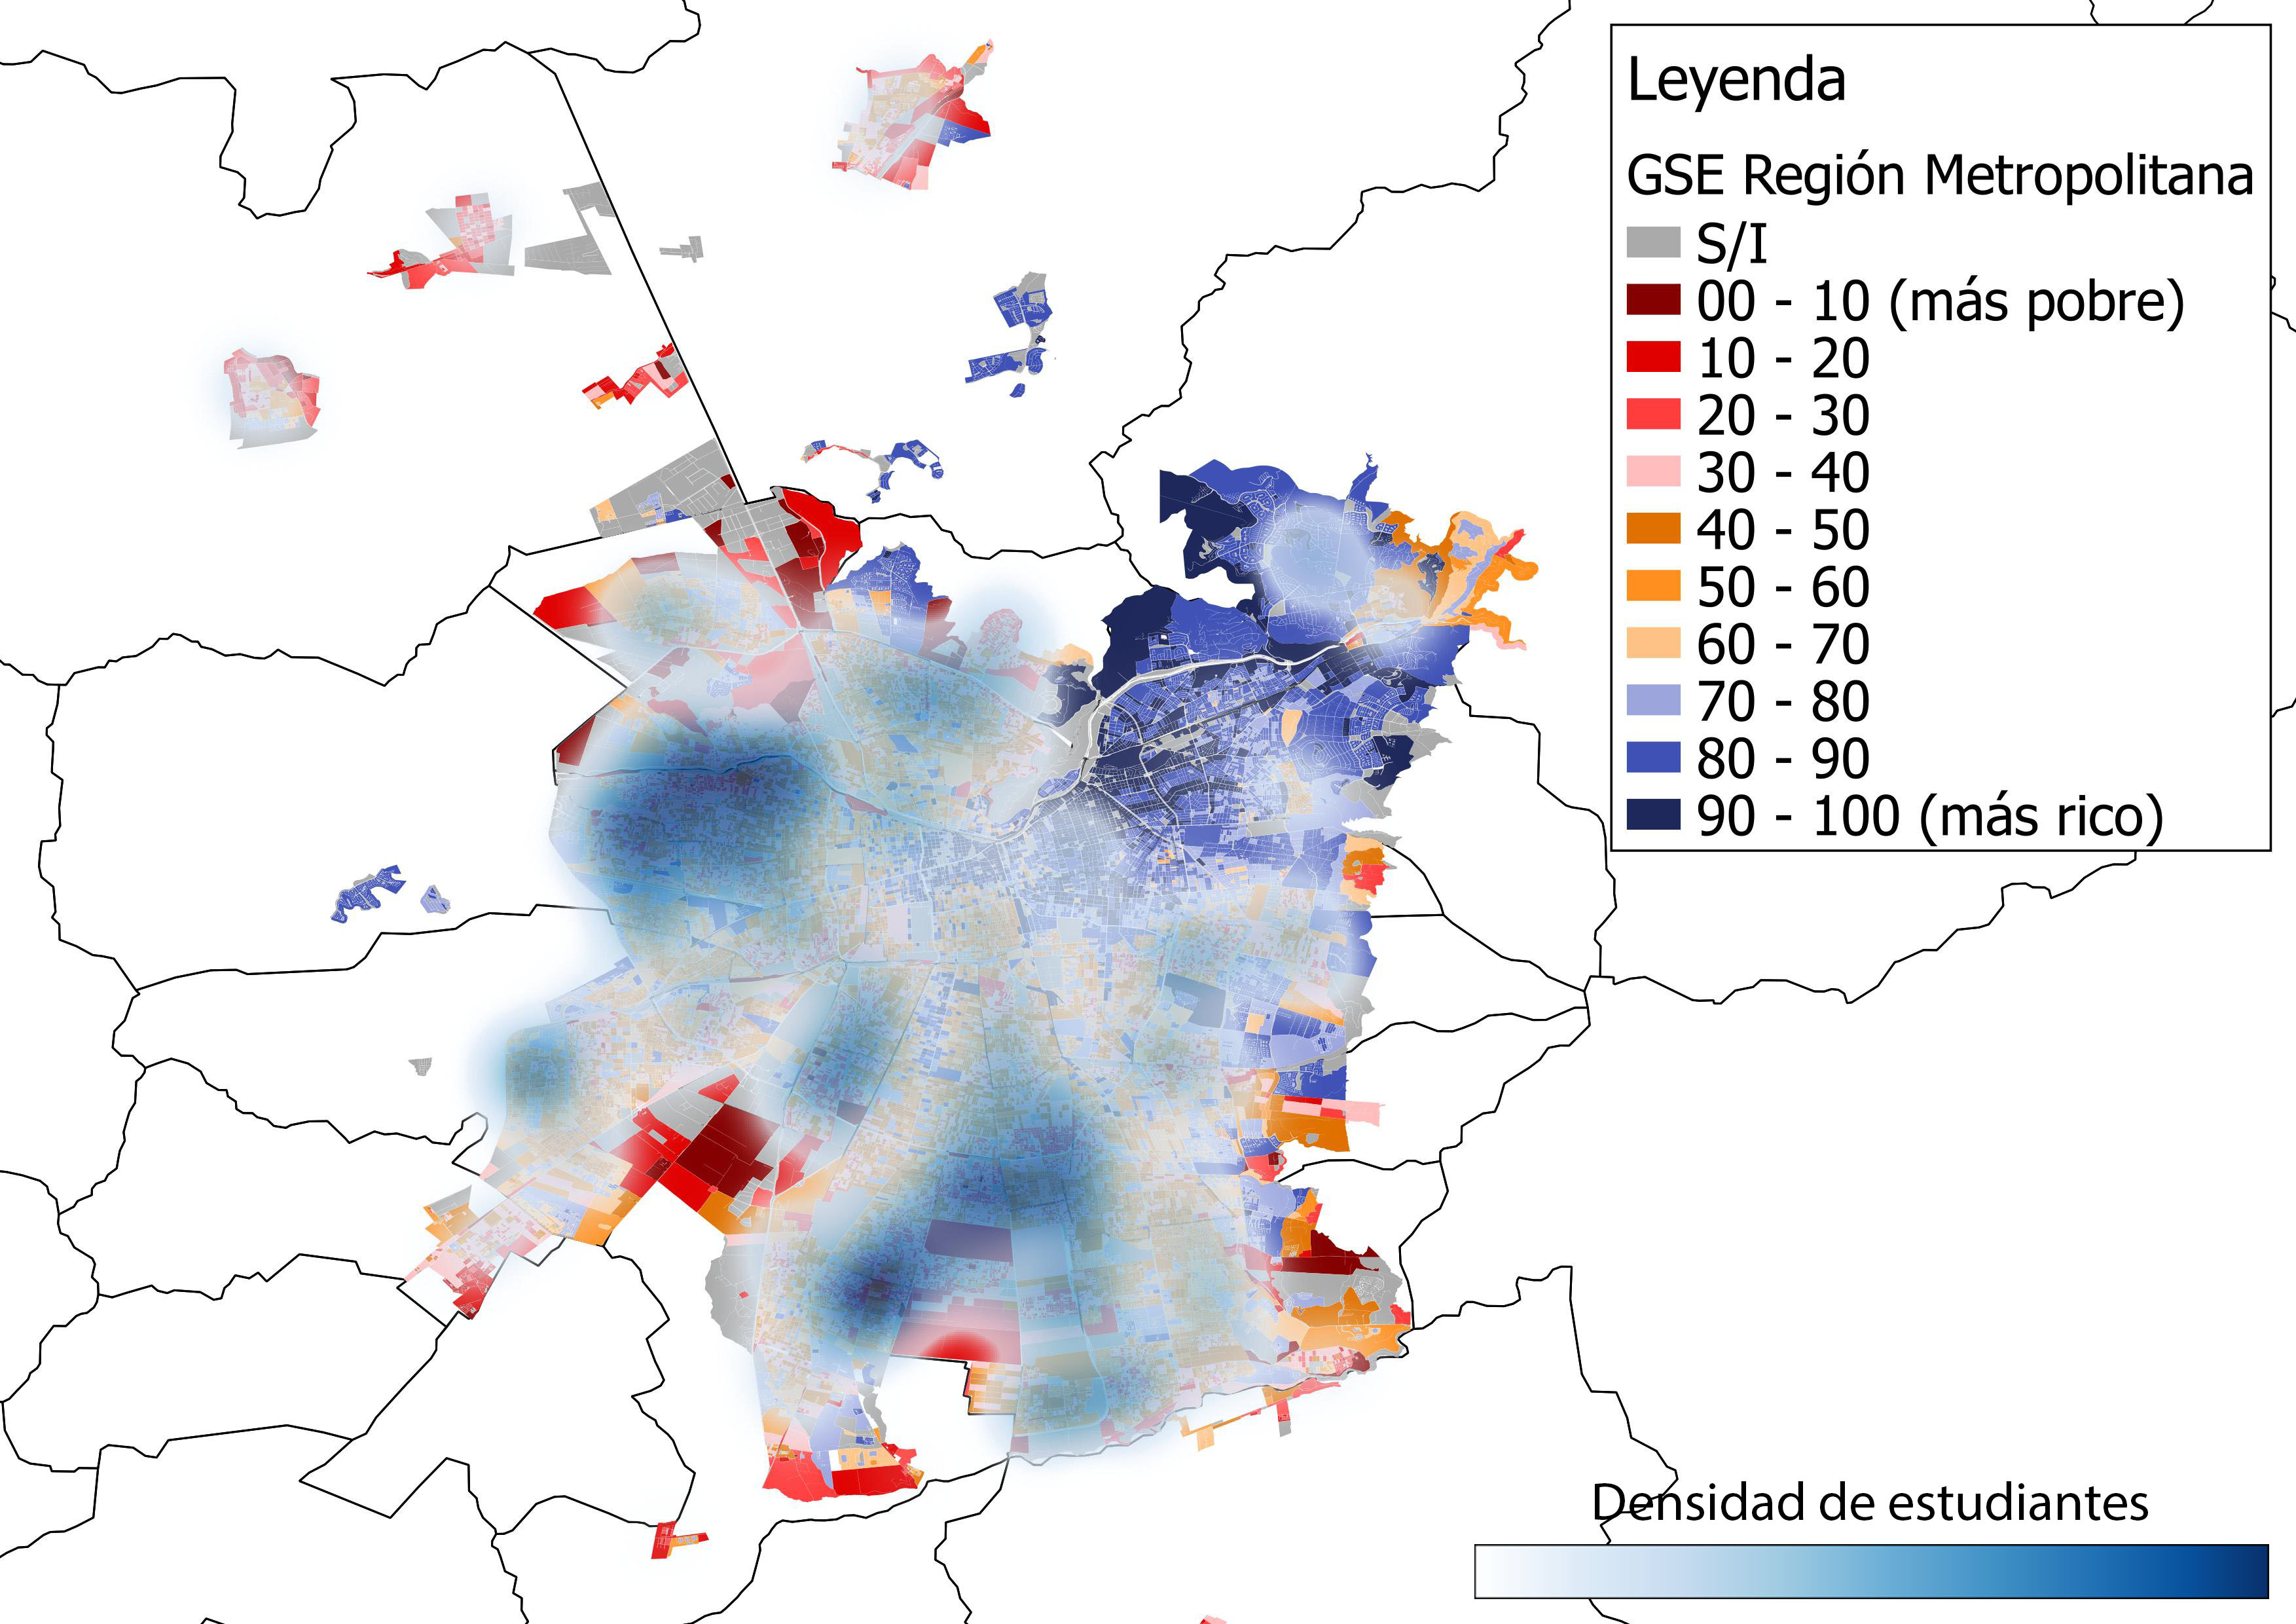
\includegraphics[width=7.5cm]{images/matriculas/M_CON_1_final.jpg}}\hspace{1mm}
  \subfloat[Matrículas clúster M\_TODAS\_CON\_2.]{
   \label{f:mapa_mat_con_2_gse}
    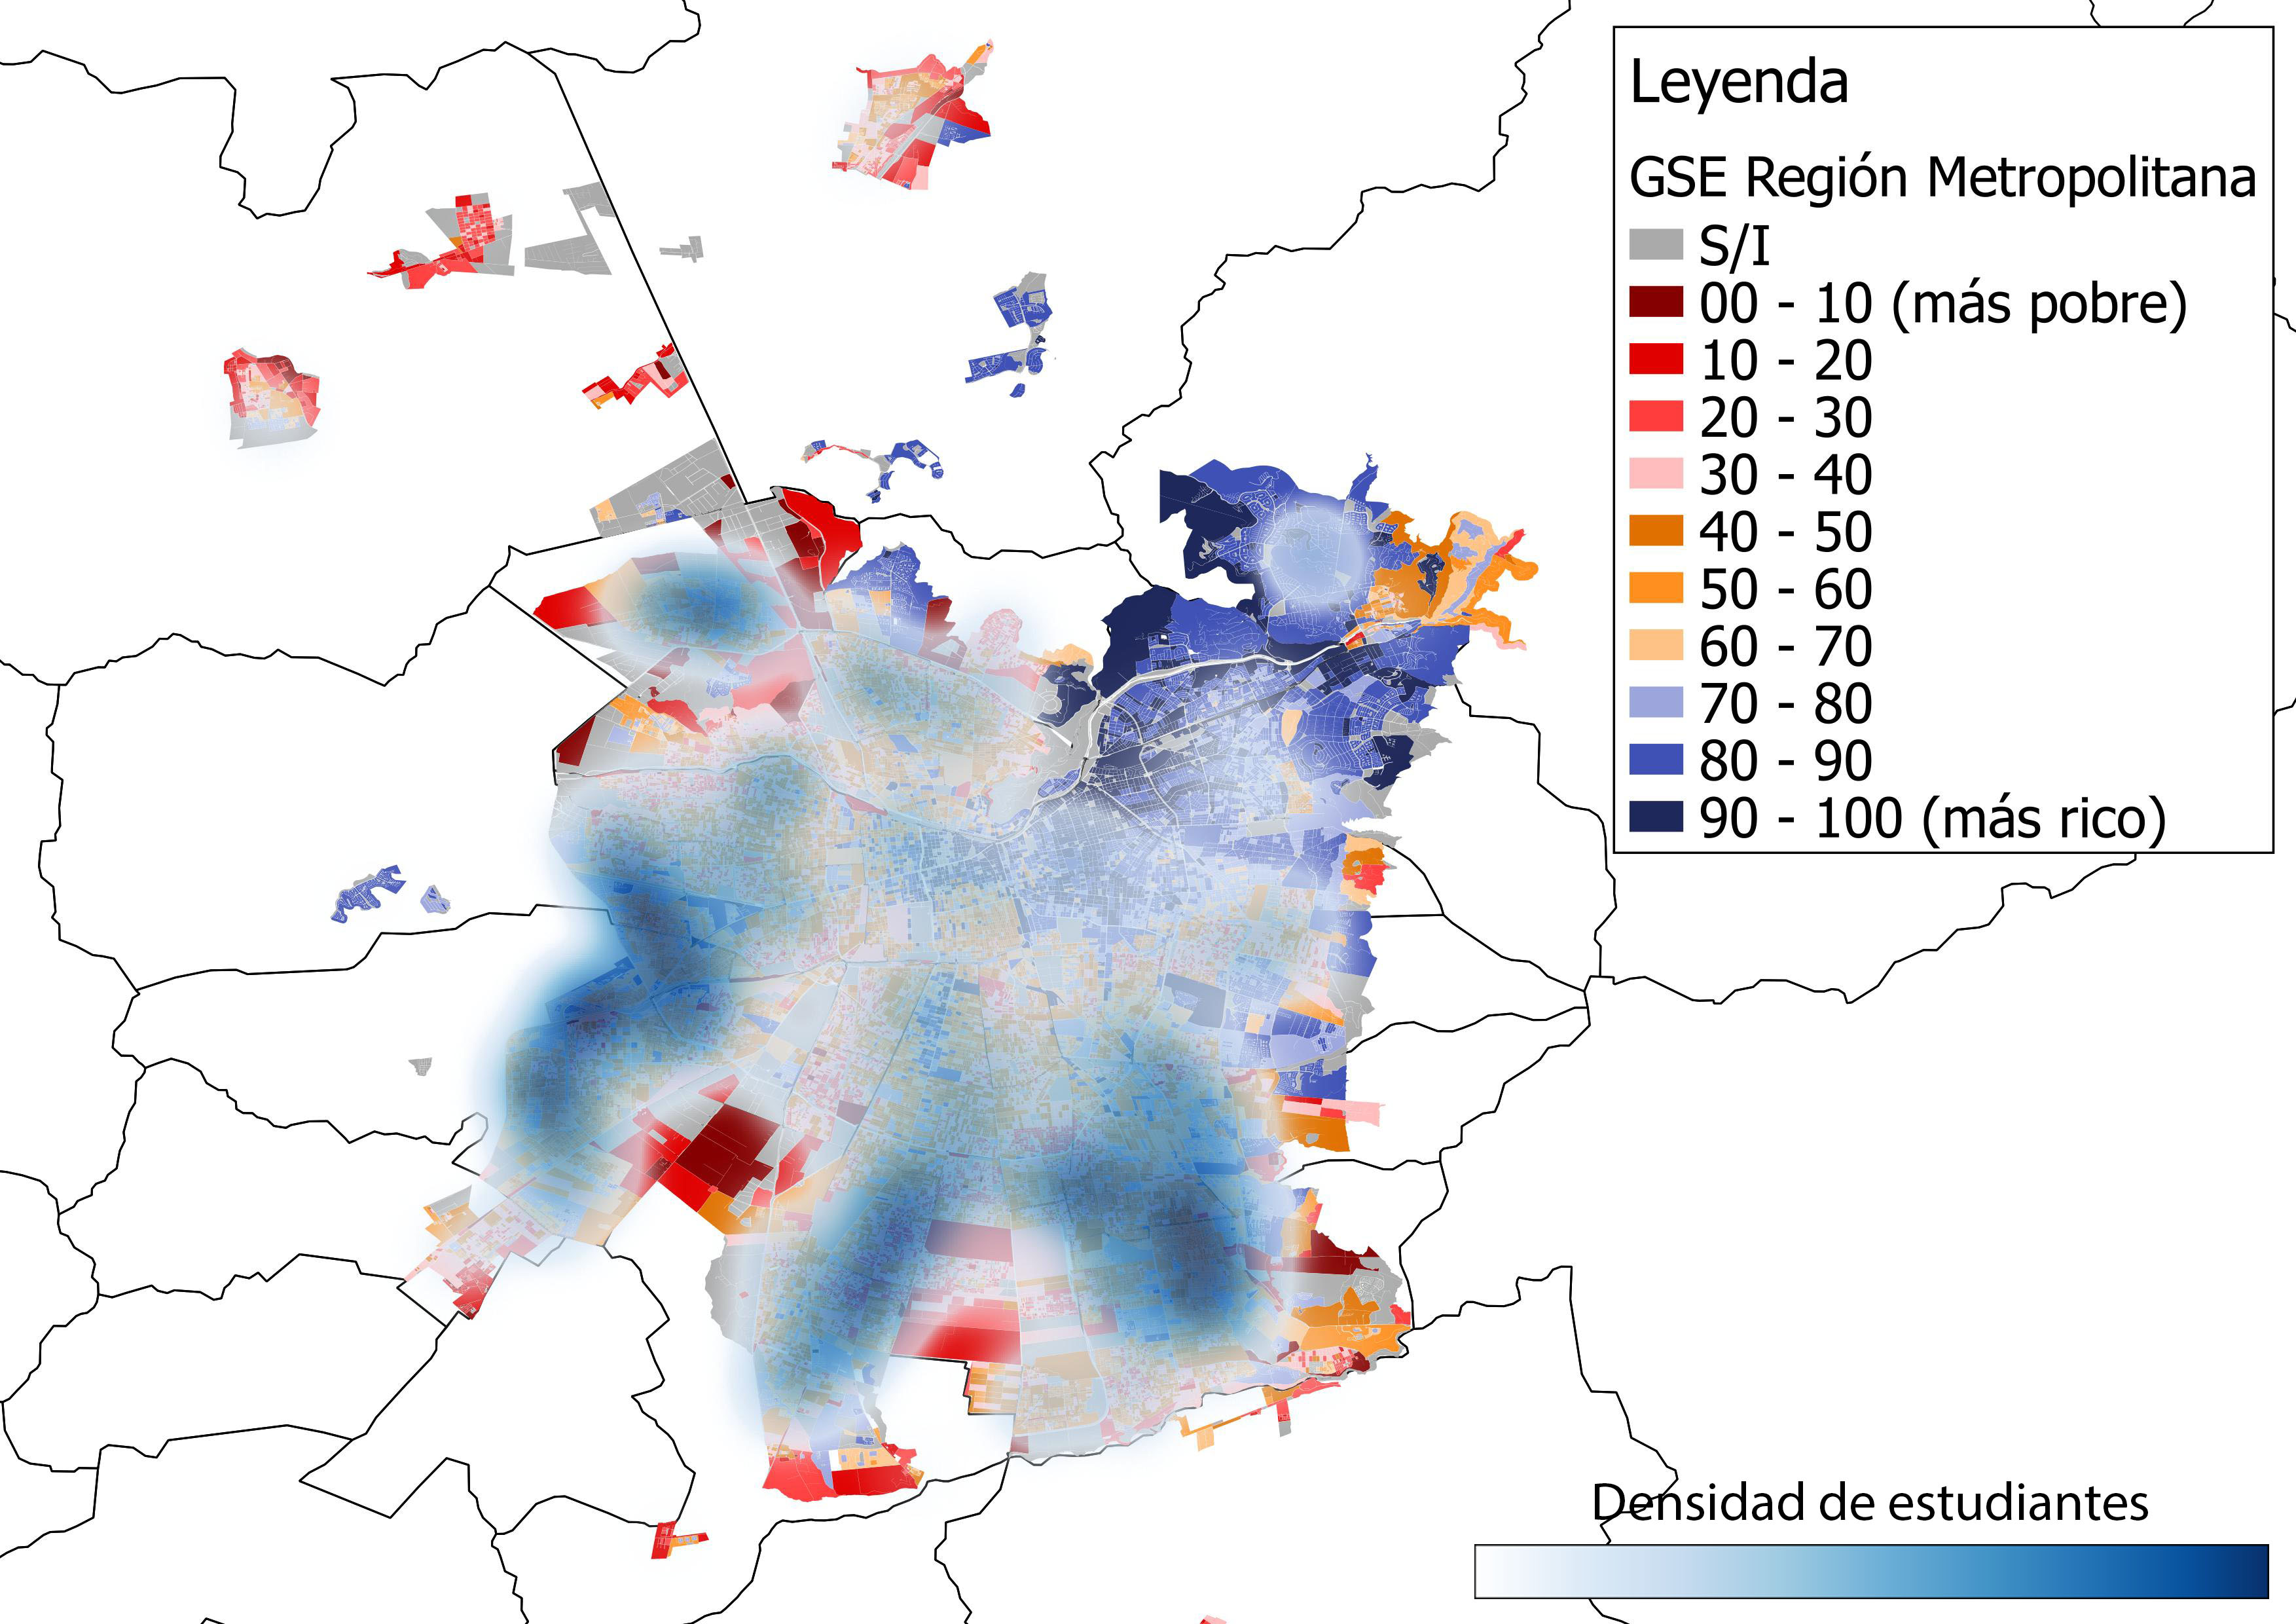
\includegraphics[width=7.5cm]{images/matriculas/M_CON_2_final.jpg}}
  \subfloat[Matrículas clúster M\_TODAS\_CON\_3.]{
   \label{f:mapa_mat_con_3_gse}
    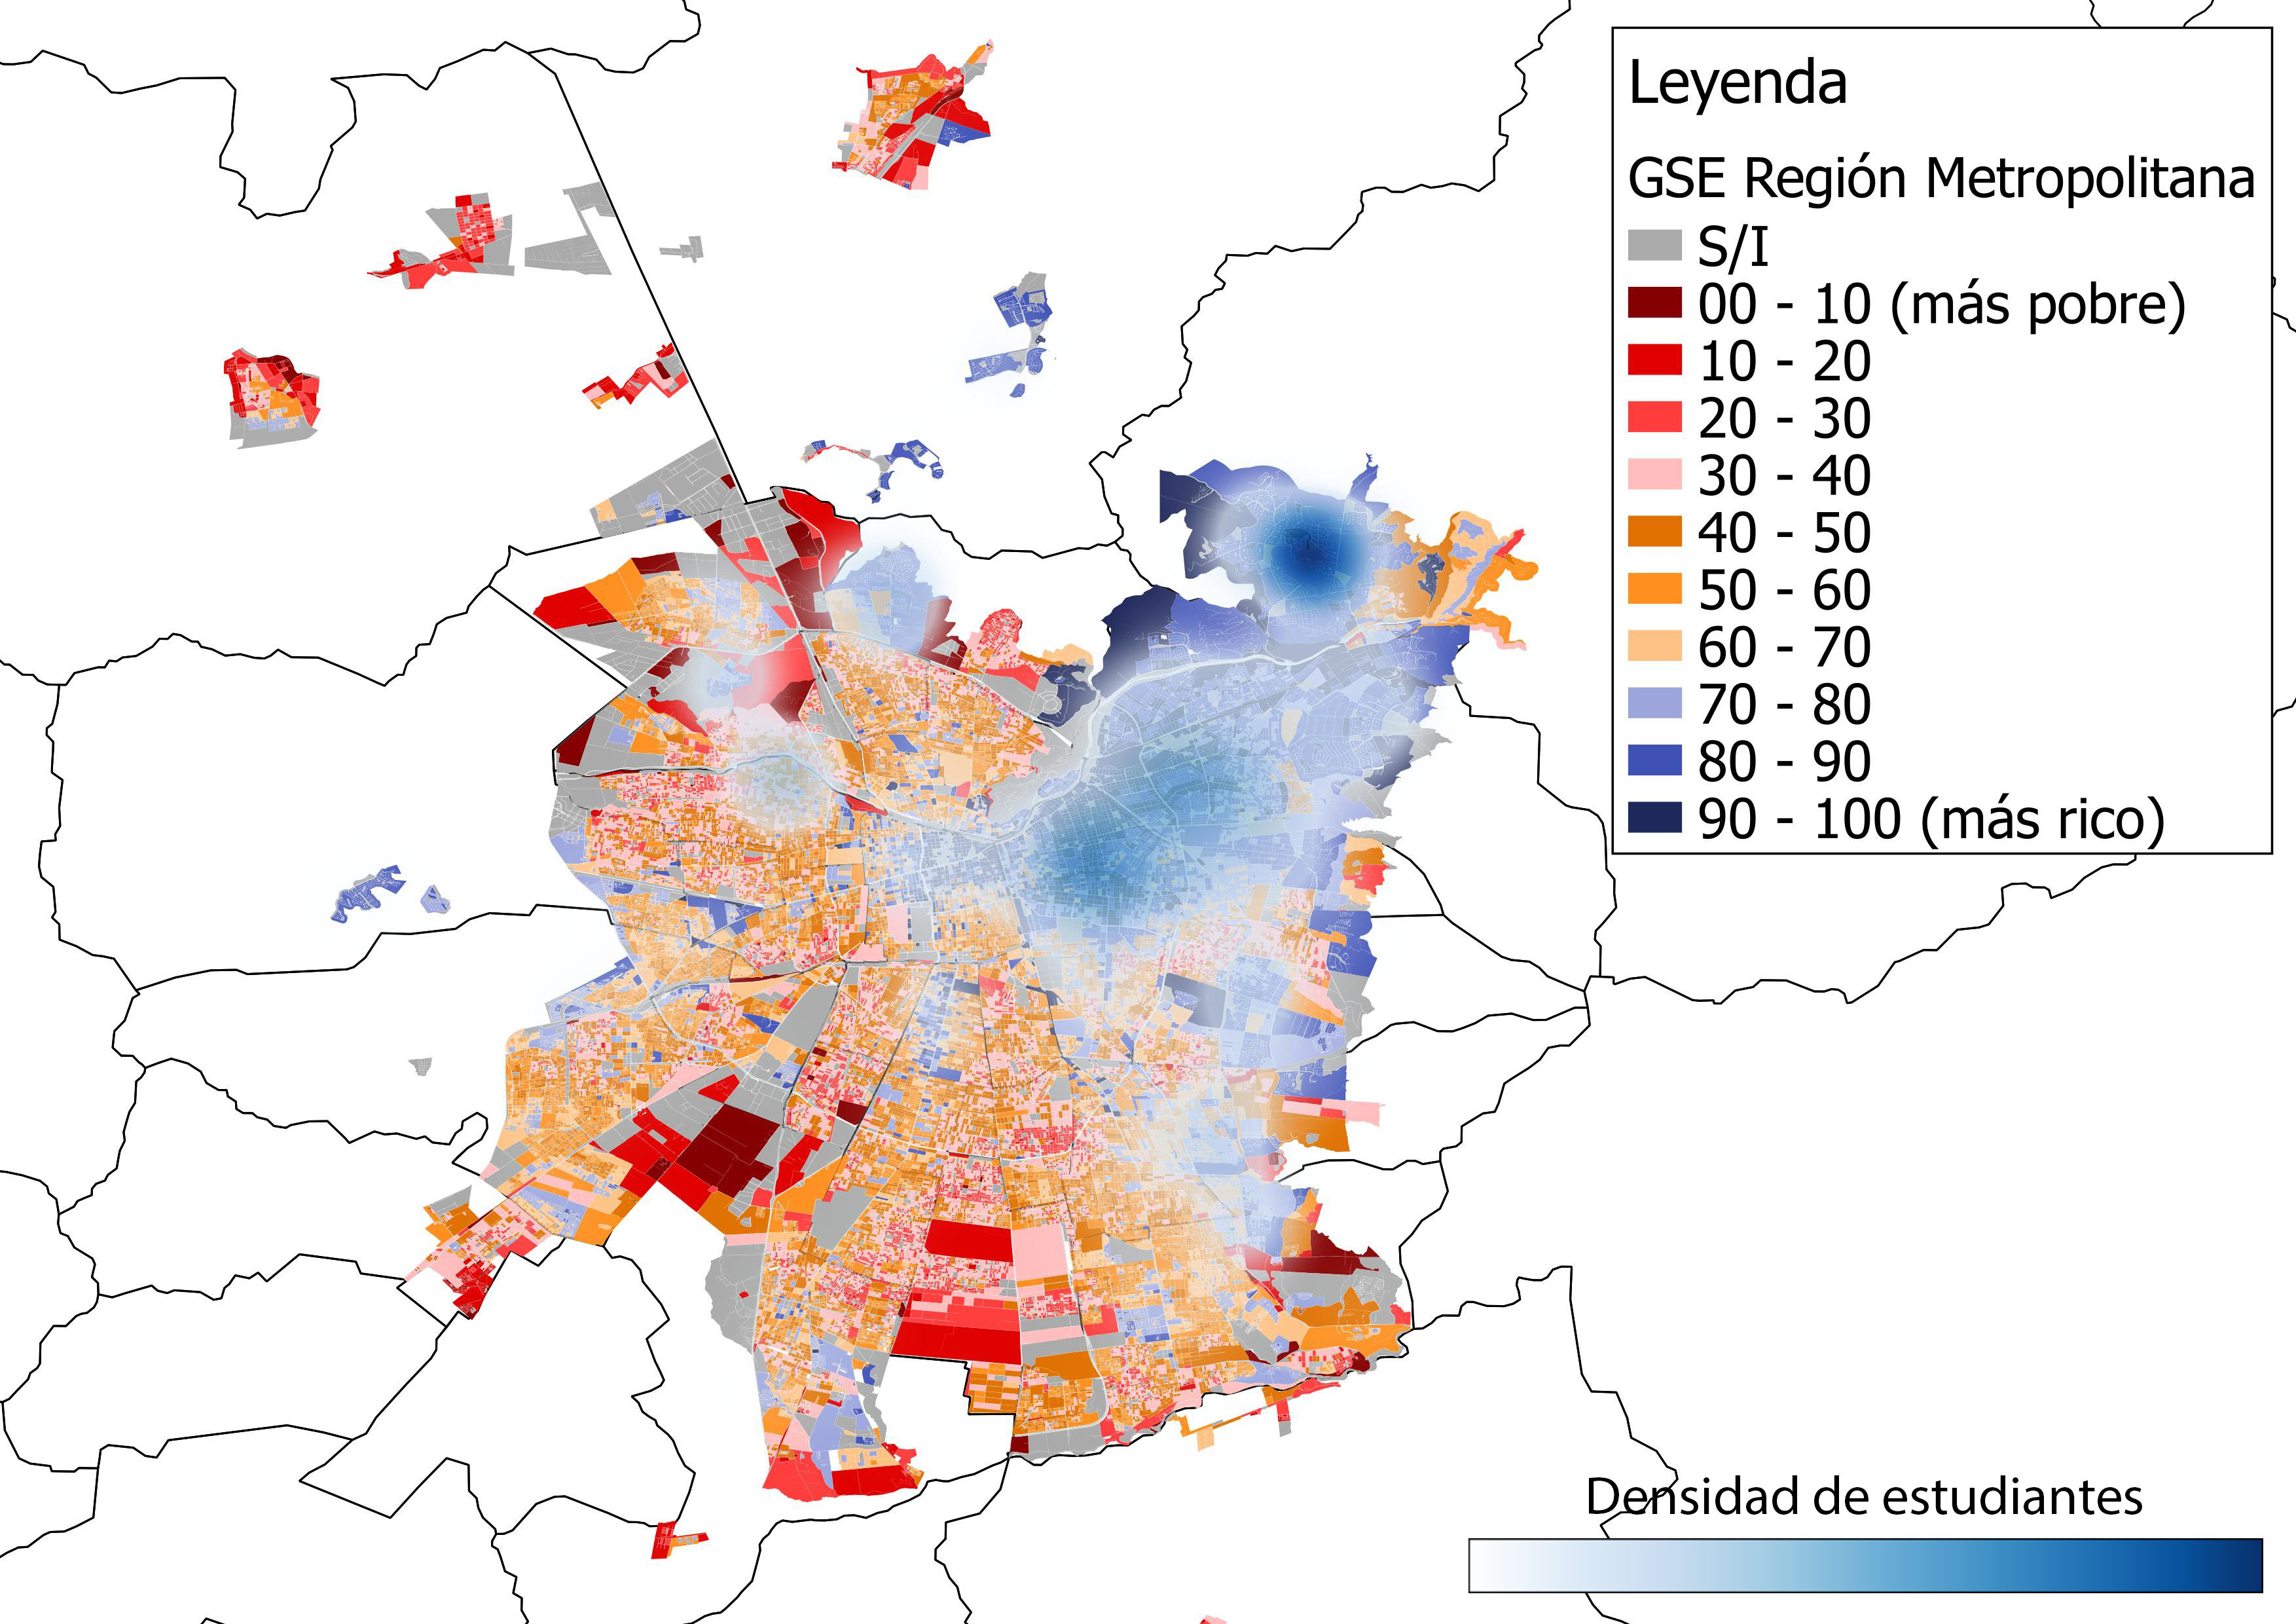
\includegraphics[width=7.5cm]{images/matriculas/M_CON_3_final.jpg}}
 \caption{Mapas de calor de clústers de matrículas (con atributos relacionales) sobre mapa GSE de la Región Metropolitana.}
 \label{f:mapas_mat_con_gse}
\end{figure}